\documentclass[withoutpreface,bwprint]{cumcmthesis} %去掉封面与编号页
\usepackage{url}%引用网站
\usepackage{cite}%引用参考文献
\usepackage{graphicx}
\usepackage{pdflscape}
\usepackage{lscape}
\usepackage{tabularx}
\usepackage{afterpage}
\usepackage{longtable}

\usepackage[numbers,sort&compress]{natbib}

\usepackage[figuresright]{rotating}
\usepackage{listings}
\usepackage{ctex}

% 设置代码样式
\lstset{
	numbers             =   left,               % 行号显示在左侧
	showspaces          =   false,              % 不显示空格符号
	numberstyle         =   \zihao{-5}\ttfamily,% 行号风格,小五号,等宽字体
	showstringspaces    =   false,              % 不显示字符串中的空格
	captionpos          =   t,                  % 标题位置在顶部
	frame               =   lrtb,               % 显示四周边框
	breaklines          =   true,               % 自动换行
	columns             =   fixed,              % 固定列宽
	basewidth           =   0.5em,              % 基础宽度
	caption             =   \raggedright,       % 标题左对齐
}

% Python 代码样式
\lstdefinestyle{Python}{
	language        =   Python, % 语言设为Python
	basicstyle      =   \zihao{-5}\ttfamily\color{black}, % 基本风格,小五号,等宽字体,黑色
	keywordstyle    =   \color{blue}\bfseries\itshape, % 关键字风格,蓝色加粗斜体
	stringstyle     =   \color{magenta}, % 字符串风格,洋红色
	commentstyle    =   \color{red}\itshape, % 注释风格,红色斜体
}

% MATLAB 代码样式
\lstdefinestyle{MATLAB}{
	language        =   Matlab, % 语言设为MATLAB
	basicstyle      =   \zihao{-5}\ttfamily\color{black}, % 基本风格,小五号,等宽字体,黑色
	keywordstyle    =   \color{green}\bfseries\itshape, % 关键字风格,绿色加粗斜体
	stringstyle     =   \color{purple}, % 字符串风格,紫色
	commentstyle    =   \color{gray}\itshape, % 注释风格,绿色斜体
}



\usepackage{xcolor}
\usepackage{multicol}

\usepackage{booktabs}
\usepackage{hyperref}
\usepackage{subcaption}
\usepackage {float} 
\usepackage{array}
\hypersetup{hidelinks,
	colorlinks=true,
	allcolors=black,
	pdfstartview=Fit,
	breaklinks=true
}
\usepackage{siunitx}

\title{基于多元回归与优化模型对 C4 烯烃制备工艺的研究}
%\tihao{A}					%题号
%\baominghao{4321}			%报名号
%\schoolname{BIT}			%学校
%\yearinput{2025}			%年份
%\monthinput{08}			%月份
%\dayinput{10}				%日期

\begin{document}


\maketitle%与上面的\title对应
\begin{abstract}%摘要+摘要+摘要+摘要+摘要

	
	 \( \text{C}_4 \) 烯烃是化学工业生产与医药制造的重要基础化工原料,也是石油化工产业的基础。近年来,随着国内化工产业的不断进步, \( \text{C}_4 \) 烯烃的综合利用越来越受到重视,乙醇催化偶合制备 \( \text{C}_4 \) 烯烃逐渐进入人们的视野。因此,选择合适的催化生产工艺,实现稳定、高效生产的目标,不仅能为企业带来明显的经济效益,同时也能促进我国相关化工企业的发展。
	
	%第一段——问题重述+简要思想:首先简要叙述所给问题的背景和动机,并分别分析每个小问题的特点(以下以三个问题为例)。根据这些特点说出自己的思想:针对于问题1,采用。。。。。。。。的方法解决;针对问题2用。。。。。。。。的方法解决;针对问题3用。。。。。。。。的方法解决。
	
	
	
	%\textbf{}:加粗	
	\textbf{针对问题一},	本文首先完成全局数据清洗预处理,通过\textbf{三次样条插值}完成缺失值填补,接着对每一个催化剂组合和温度绘制折线图对比乙醇转化率和 \( \text{C}_4 \) 烯烃选择性的趋势图分析变量与温度间的关系为强正相关,又通过皮尔逊相关系数计算,可筛选出相关性最强的组合作为工艺优化对象。又对350度时给定的催化剂组合所得实验数据进行数据可视化绘制折线图,观察可得,在一定温度和相同催化剂下,随着时间的增加,反应物乙醇转化率持续下降,逐渐趋于稳定;\( \text{C}_4 \) 烯烃选择性增加,并趋于稳定,与时间呈现出弱负相关性。
	%第二段——模型建立及求解结果:介绍思想和模型: 对于问题1我们首先建立了。。。。。。。。模型I。首先利用。。。。。。,其次计算了。。。。。。,并借助。。。。。。数学算法和。。。。。。软件得出了。。。。。。结论。
	
	
	
	
	\textbf{针对问题二},依据问题一所得信息,使用\textbf{正则表达式}将催化剂组合和温度信息分离构建为独立变量,通过控制变量法分别控制装料方式不同、乙醇浓度不同、Co负载量不同、有无HAP、总质量不变,Co与HAP质量比不同以及Co与HAP质量比1:1,总质量不同进行实验对比可得,温度对两因变量影响最强且不易受干扰,其他因素都对因变量影响较弱但不可忽略。
	%(第3段)	对于问题2我们用。。。。。。。。
	
	
	
	\textbf{针对问题三},探究多个自变量与在相同的实验条件下,如何组合从而使得 \( \text{C}_4 \) 烯烃的收率最大。通过题中所给的 \( \text{C}_4 \) 烯烃收率计算式,写出全数据收率结果,在此基础上构建\textbf{多项式回归},训练成功后使用\textbf{网格搜索}得到温度限制在450°C时, \( \text{C}_4 \) 烯烃最大收率为52.03\%;当温度限制在350°C时, \( \text{C}_4 \) 烯烃最大收率为21.70\%。
	%(第4段)	对于问题3我们用。。。。。。。。(模型的建立与求解结果的陈述中,思想、模型、软件和结果必须描述清晰,亮点详细说明需突出。针对不同问题可独立成段也可采用一段式仅用分号“;”分割,摘要只接受文字描述形式,不接受图表等其他方式)
	
	\textbf{针对问题四},基于前三问模型结论,采用模型驱动的序贯实验设计策略精准规划五次实验:首先在450℃(全局最优预测点)和350℃(低温最优点)执行确认实验,验证模型外推可靠性;其次依据岭回归分析(Co负载量与选择性负相关),在A3基础上将Co负载量提升至8wt\%,实施极值寻优以探测参数拐点;针对催化剂失活问题,第四组延长反应时间至400分钟,构建加速寿命测试量化失活动力学;第五组在B装料方式下复现高温条件,通过对照实验检验工艺泛化能力。设计遵循"模型预测→靶向实验→反馈修正"动态闭环,五次实验分别覆盖参数验证、边界探索、稳定性评估及系统适应性检验,以单次实验信息增量最大化为目标,在有限次数内高效逼近最优工艺,显著提升研究效率与科学性。
	
	
	
	%(第5段)	优化结果及总结:在。。。。。。条件下,针对。。。。。。模型进行适当修改与优化,这种条件的改变可能来自你的一种猜想或建议。要注意合理性。此推广模型可以不深入研究,也可以没有具体结果。
	
	%注:字数300~600之间,需控制在一页;摘要中必须将具体方法、模型和所得结果写出来;摘要要求“总分总”,段开头可用“针对问题1,针对问题2,针对问题3..”或者“首先,然后,其次,最后”等词语进行有逻辑的论述。摘要是重中之重,必须严格执行!
	
	
	
	\keywords{\textbf{三次样条插值}\quad  \textbf{正则表达式}\quad   \textbf{岭回归}\quad   \textbf{多项式回归}\quad \textbf{网格搜索}}
	%\keywords:关键词;\quad:空格
	%使用到的模型名称、方法名称、特别是亮点一定要在关键字里出现,3~5个较合适,用分号隔开
\end{abstract}
%摘要  abstract.tex

%\section{}-subsection{}-subsubsection{}:标题1-3级
\section{问题背景与重述}
\subsection{问题背景}
%在保持原题主体思想不变下,可以自己组织词句对问题进行描述,主要数据可以直接复制,对所提出的问题部分基本原样复制。篇幅建议不要超过一页。大部分文字提炼自原题。)
 \( \text{C}_4 \) 烯烃可用于生产聚丙烯等多项化工产品,是重要的基础化工原料,是优质的汽油调和组分,是石油化工产业的基础。近些年,随着国内煤化工业的不断发展, \( \text{C}_4 \) 烯烃的综合利用越来越受到重视,乙醇催化偶合制备 \( \text{C}_4 \) 烯烃逐渐进入人们的视野。

因此,选择合适的催化生产工艺,达到稳定、高效生产的目的,提高 \( \text{C}_4 \) 烯烃的选择性和收率,不仅能为企业带来明显的经济效益,同时也能促进我国相关化工企业的发展。







\subsection{问题重述}
%结合以上情况,建立数学模型解决以下问题:
某化工实验室针对不同催化剂在不同温度下做了一组实验,结果如附件 1 和附件 2 所示。请通过数学建模完成下列问题:

\begin{enumerate}
	\item 问题一:针对附件 1 所给的催化剂组合,研究其乙醇转化率、 \( \text{C}_4 \) 烯烃的选择性与温度的关系;并分析附件 2 所给定的催化剂组合在一次实验中 350℃ 下不同时间的实验结果进行分析。
	
	\item 问题二:研究不同催化剂组合和温度对乙醇转化率和 \( \text{C}_4 \) 烯烃选择性的影响。
	
	\item 问题三:如何选择催化剂组合与温度,使得在相同实验条件下 \( \text{C}_4 \) 烯烃收率尽可能高?若使温度低于 350 度,又如何选择催化剂组合与温度,使得 \( \text{C}_4 \) 烯烃收率尽可能高?
	
	\item 问题四:如果允许再增加五次实验,应如何设计,并给出详细理由。
\end{enumerate}%插入问题重述   ProblemRestatement.tex

\newpage
\section{问题分析}
%TOPS:这部分写差不多一页(删掉此句话)
\subsection{问题一分析}
对于问题一,第一部分的问题,可以分别针对两种装料方式的十九中不同催化剂组合所得实验结果绘制折线图,根据折线图及分析可得各催化剂组合温度和 \( \text{C}_4 \) 烯烃选择性以及乙醇转化率的关系,同时可计算变量之间的相关性,绘制分布气泡图。第二部分的问题根据附件二所给额外实验数据做分析,绘制折线图,由于其他变量都是由于催化剂组合不同和温度不同造成的结果,不需要做主成分分析进行降维,直接分析即可。



\subsection{问题二分析} 
对于问题二,要求探讨不同催化剂组合及温度对乙醇转化率以及 \( \text{C}_4 \) 烯烃选择性大小的影响,可以通过控制变量法分组进行比较,如装料方式不同、乙醇浓度不同、Co负载量不同、有无HAP、Co与HAP质量比不同以及总质量不同等可控变量,进行分组后分别比较。为了弄清催化剂类型对他们的影响,可以对催化剂进行文本数据提取,并将 \( \text{C}_4 \) 烯烃选择性和乙醇转化率分别作为因变量,以催化剂数据作为自变量构建岭回归得到相关关系。



\subsection{问题三分析}
对于问题三,要选择使得 \( \text{C}_4 \) 烯烃收率达到最高的催化剂组合和温度,我们可以在问题二拆解催化剂数据的基础上首先全局选取收率最高的催化剂组合再控制温度在350度以下选取局部收率最高的催化剂组合。由于这样只是选出了在数据面上的优选项,我们可以通过建立多项式回归模型,在连续的参数空间内进行网格搜索,以预测理论上可达到的最高C4烯烃收率及其对应的催化剂组合和温度。




\subsection{问题四分析}
对于问题四,综合前三问所的结果,考虑在催化剂组合和温度的各个参数变化方向上进行调整,选出最合适的五个实验环境,最大化信息获取 ,从而更有效地逼近最优的工艺条件。


%插入问题分析    ProblemAnalysis.tex

\newpage%\新一页
\section{模型的假设}
为了构建更为精确的数学模型,本文根据实际情况做出以下合理的假设或条件约束:
%1.	假设题目所给的数据真实可靠;
%注意:假设对整篇文章具有指导性,有时决定问题的难易。一定要注意假设的某种角度上的合理性,不能乱编,完全偏离事实或与题目要求相抵触。注意罗列要工整。
\begin{enumerate}
	\item 乙醇催化偶合制备 \( \text{C}_4 \) 烯烃的过程中,除给定催化剂组合以及温度和反应时间外,其它条件对实验结果的影响可忽略不计。
	\item 在反应进行时,实验室内环境温度和气压不会对反应造成影响。
	\item 实验设备完好且在实验过程中不会出现漏气、破损等情况导致实验失败或数据出现差错。
	\item 在实验条件下,逆反应速率极慢,且 \( \text{C}_4 \) 烯烃生成后迅速脱离反应体系,从而逆反应影响可以忽略。
\end{enumerate}

\section{符号说明}
\begin{table}[H] %[h]表示在此处添加浮动体,默认为tbf,即页面顶部、底部和空白处添加
	\captionsetup{skip=4pt} % 设置标题与表格的间距为4pt
	\centering
	\setlength{\arrayrulewidth}{1pt} % 设置表格线条宽度为1pt
	\begin{tabular}{cc} %c表示居中,l表示左对齐,r表示右对齐,中间添加“|”表示竖线
		\hline
		\makebox[0.15\textwidth][c]{符号} & \makebox[0.6\textwidth][c]{说明}  \\ 
		\hline
		$X$ & 乙醇转化率 \\
		$S$ & C4烯烃选择性 \\
		$Y$ & C4烯烃收率($Y = X \times S$) \\
		$r$ & 皮尔逊相关系数 \\
		$\lambda$ & 岭回归正则化参数(惩罚系数) \\
		$\alpha$ & 岭回归模型通过交叉验证得到的最优正则化参数 \\
		$w$ & 岭回归模型的回归系数向量 \\
		$R^2$ & 决定系数,用于评估模型拟合优度 \\
		$n$ & 样本数量 \\
		$i, j$ & 求和或循环中的索引变量 \\
		$\bar{x}, \bar{y}$ & 变量 $x$ 和 $y$ 的均值 \\
		\hline
	\end{tabular}
	% \hline是横线,采用\makebox设置列宽
\end{table}


%插入模型假设及符号说明  AssumptionAndSign.tex

\newpage	
\section{模型的建立与求解}
\subsection{数据的预处理}

题目所给两个附件,首先观察,附件一中包含大量合并单元格,python的pandas读取后会造成大量缺失,需要进行填充,而附件二也包含合并单元格,但是有无用内容,我们直接手动删去标题以及合并的单元格后使用python读取。针对附件一的处理,使用pandas读取后,使用ffill()方法向下填充,同时简单检查缺失值。

关于附件一的温度跳跃现象,暂时不做处理,在后续题目作答过程中视需要进行填补或插值处理。


\subsection{问题一的模型建立与求解}
\subsubsection{三次样条插值}
对每种催化剂组合内分析三者之间的关系,由于每组内样本数量较少,且温度之间差值较大,直接绘制图像影响图像的连贯性,这里使用三次样条插值完成对中间间距大于25的数据的插值,包括温度,乙醇转化率以及 \( \text{C}_4 \) 烯烃选择性。三次样条插值的计算方式如下:

令 \( S(x) \) 在每个区间 \([x_i, x_{i+1}]\) 上为一个三次多项式:
\[
S_i(x) = a_i + b_i(x - x_i) + c_i(x - x_i)^2 + d_i(x - x_i)^3
\]

其中 \( i = 0, 1, \dots, n-1 \),共 \( n \) 个区间。三次样条插值求解较为复杂,这里使用python的scipy.interpolate函数实现。

\subsubsection{数据可视化}
为了更直观展示乙醇转化率和 \( \text{C}_4 \) 烯烃选择性与温度之间的关系,我们对各催化剂组合和温度下的数据进行可视化,绘制折线图如图1:

\begin{figure}[h]%[h]:固定作用
	\centering%置中
	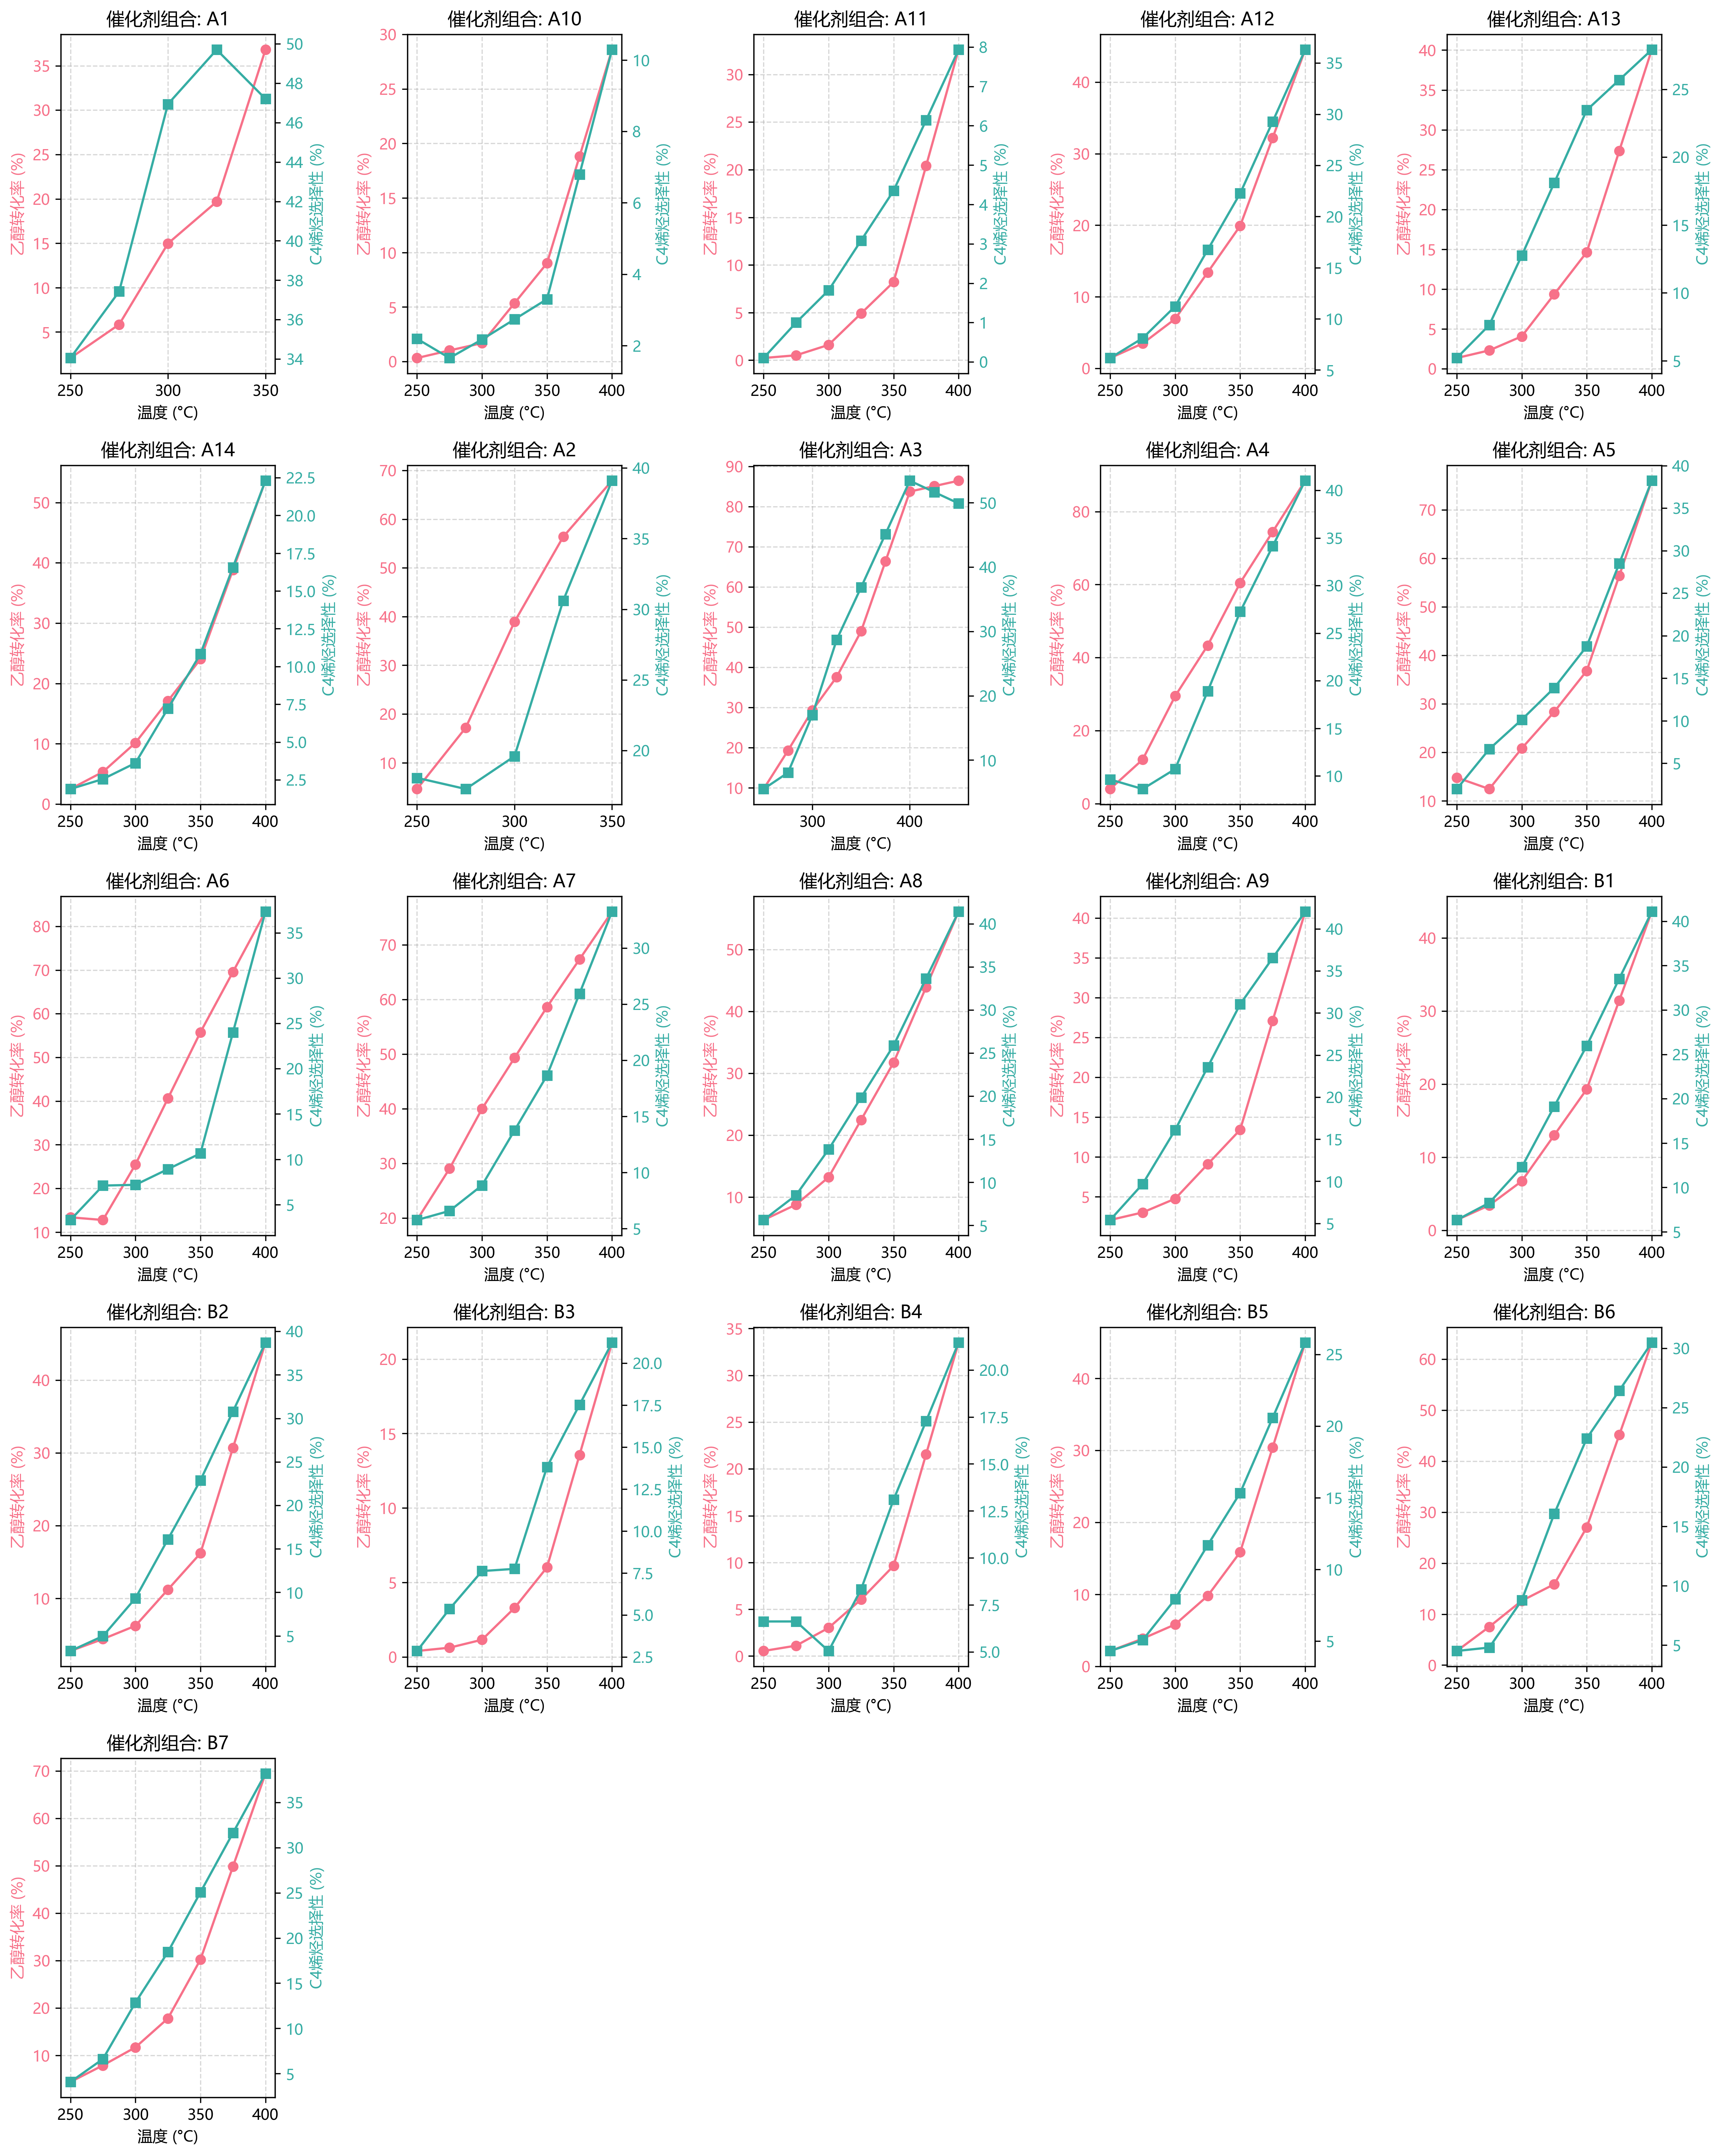
\includegraphics [scale=0.4]{图/1-1-1.png}
	\caption{乙醇转化率和C4烯烃选择性与温度的关系} 
	\label{fig:1}
\end{figure}

\newpage

大致可以发现折线有两种整体趋势为增长的形态,一种为单调递增,另一种为先少量下降再上升。首先单调递增可直接理解为温度上升,催化剂活性增强,使反应进行更彻底;另一种先下降再上升,在拐点之前催化剂活性上升,但目标产物反应不及其他副产物,也可能由于低温情况下催化剂表面的吸附-脱附平衡不利,导致有效反应速率下降。

\subsubsection{相关性计算与比较}
对各催化剂组合中的乙醇转化率和 \( \text{C}_4 \) 烯烃选择性分别与温度计算皮尔逊相关系数,这一参数可以比较两个变量之间的相关性,大小处于-1到1之间,绝对值越高相关性越高,正代表正相关,负代表负相关,皮尔逊相关系数的计算公式为:

$$
r = \frac{\sum_{i=1}^{n} (x_i - \bar{x})(y_i - \bar{y})}{\sqrt{\sum_{i=1}^{n} (x_i - \bar{x})^2} \cdot \sqrt{\sum_{i=1}^{n} (y_i - \bar{y})^2}}
$$

其中:
 $ \bar{x} $ 是 $ X $ 的均值,
 $ \bar{y} $ 是 $ Y $ 的均值。Python的numpy包内置了函数可直接得到相关系数,部分数据如表1:
 
\begin{table}[!htbp]
	\caption{催化剂组合在不同温度下的乙醇转化率与C4烯烃选择性相关系数(部分)}
	\centering
	\begin{tabular}{c c c}
		\hline
		\multicolumn{1}{c}{催化剂组合} & \multicolumn{1}{c}{乙醇转化率-温度 (r)} & \multicolumn{1}{c}{C4烯烃选择性-温度 (r)} \\
		\hline
		A1  & 0.9655 & 0.8871 \\
		A2  & 0.9950 & 0.9143 \\
		B1  & 0.9621 & 0.9858 \\
		B2  & 0.9293 & 0.9848 \\
		\hline
	\end{tabular}
	\label{tab:1}
\end{table}

最终详细相关系数见附录。针对该相关系数表格做气泡图,横轴为乙醇转化率与温度的皮尔逊相关系数,纵轴为C4烯烃选择性与温度的皮尔逊相关系数,同时发现恰好两轴均为0.95处引出两条线可将所有气泡分为四部分,所绘气泡图如下:

\begin{figure}[h]%[h]:固定作用
	\centering%置中
	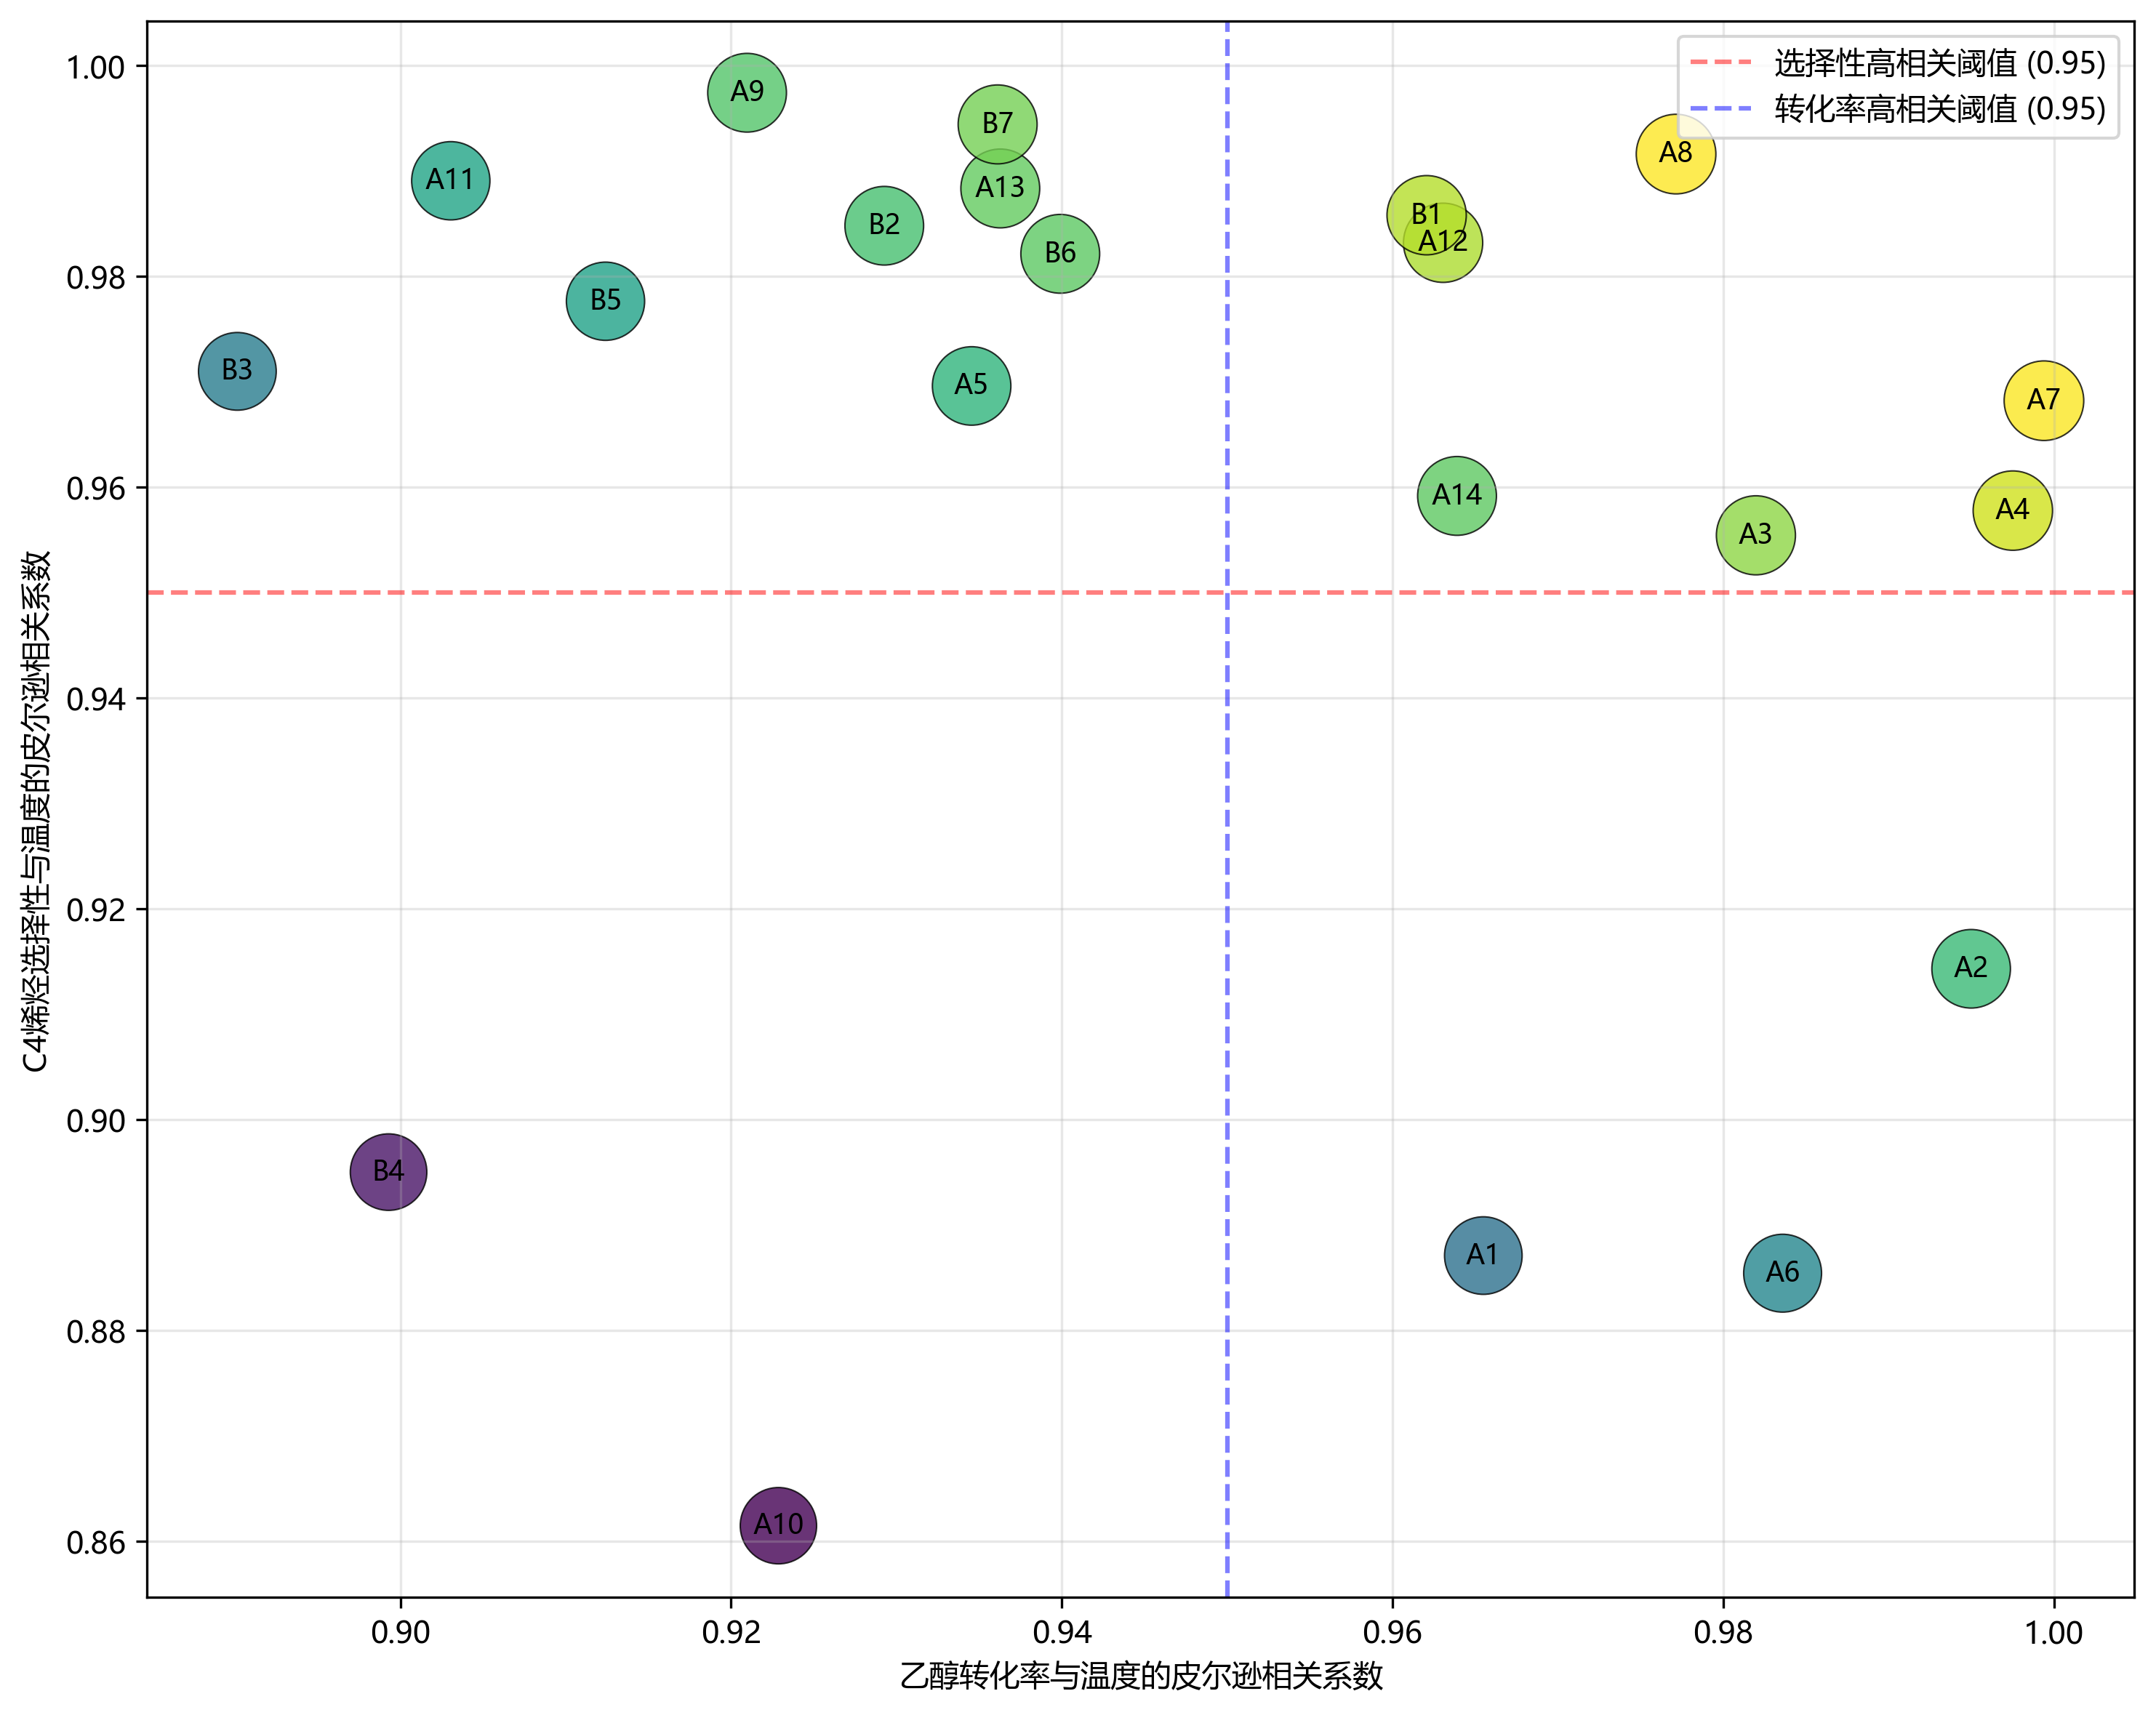
\includegraphics [scale=0.6]{图/1-2-2.png}
	\caption{各催化剂组合双指标相关性分布} 
	\label{fig:1}
\end{figure}

\newpage

所有的催化剂组合都具有高相关性,即这些催化剂组合对温度而变化十分敏感,这与温度升高,催化剂活性升高相符。图中右上角的催化剂组合是所给数据中可能更容易通过调节温度来优化反应条件,从而实现高转化率和高选择性的双重目标的组合。

\subsubsection{给定测试结果分析}
针对附件二所给某种催化剂组合的测试数据进行分析,是不同变量随时间变化的表格数据,由于该工艺的原料和产物分别是乙醇和 \( \text{C}_4 \) 烯烃,只需要主要关注这两者随时间变化即可,绘制折线图如下:

\begin{figure}[h]%[h]:固定作用
	\centering%置中
	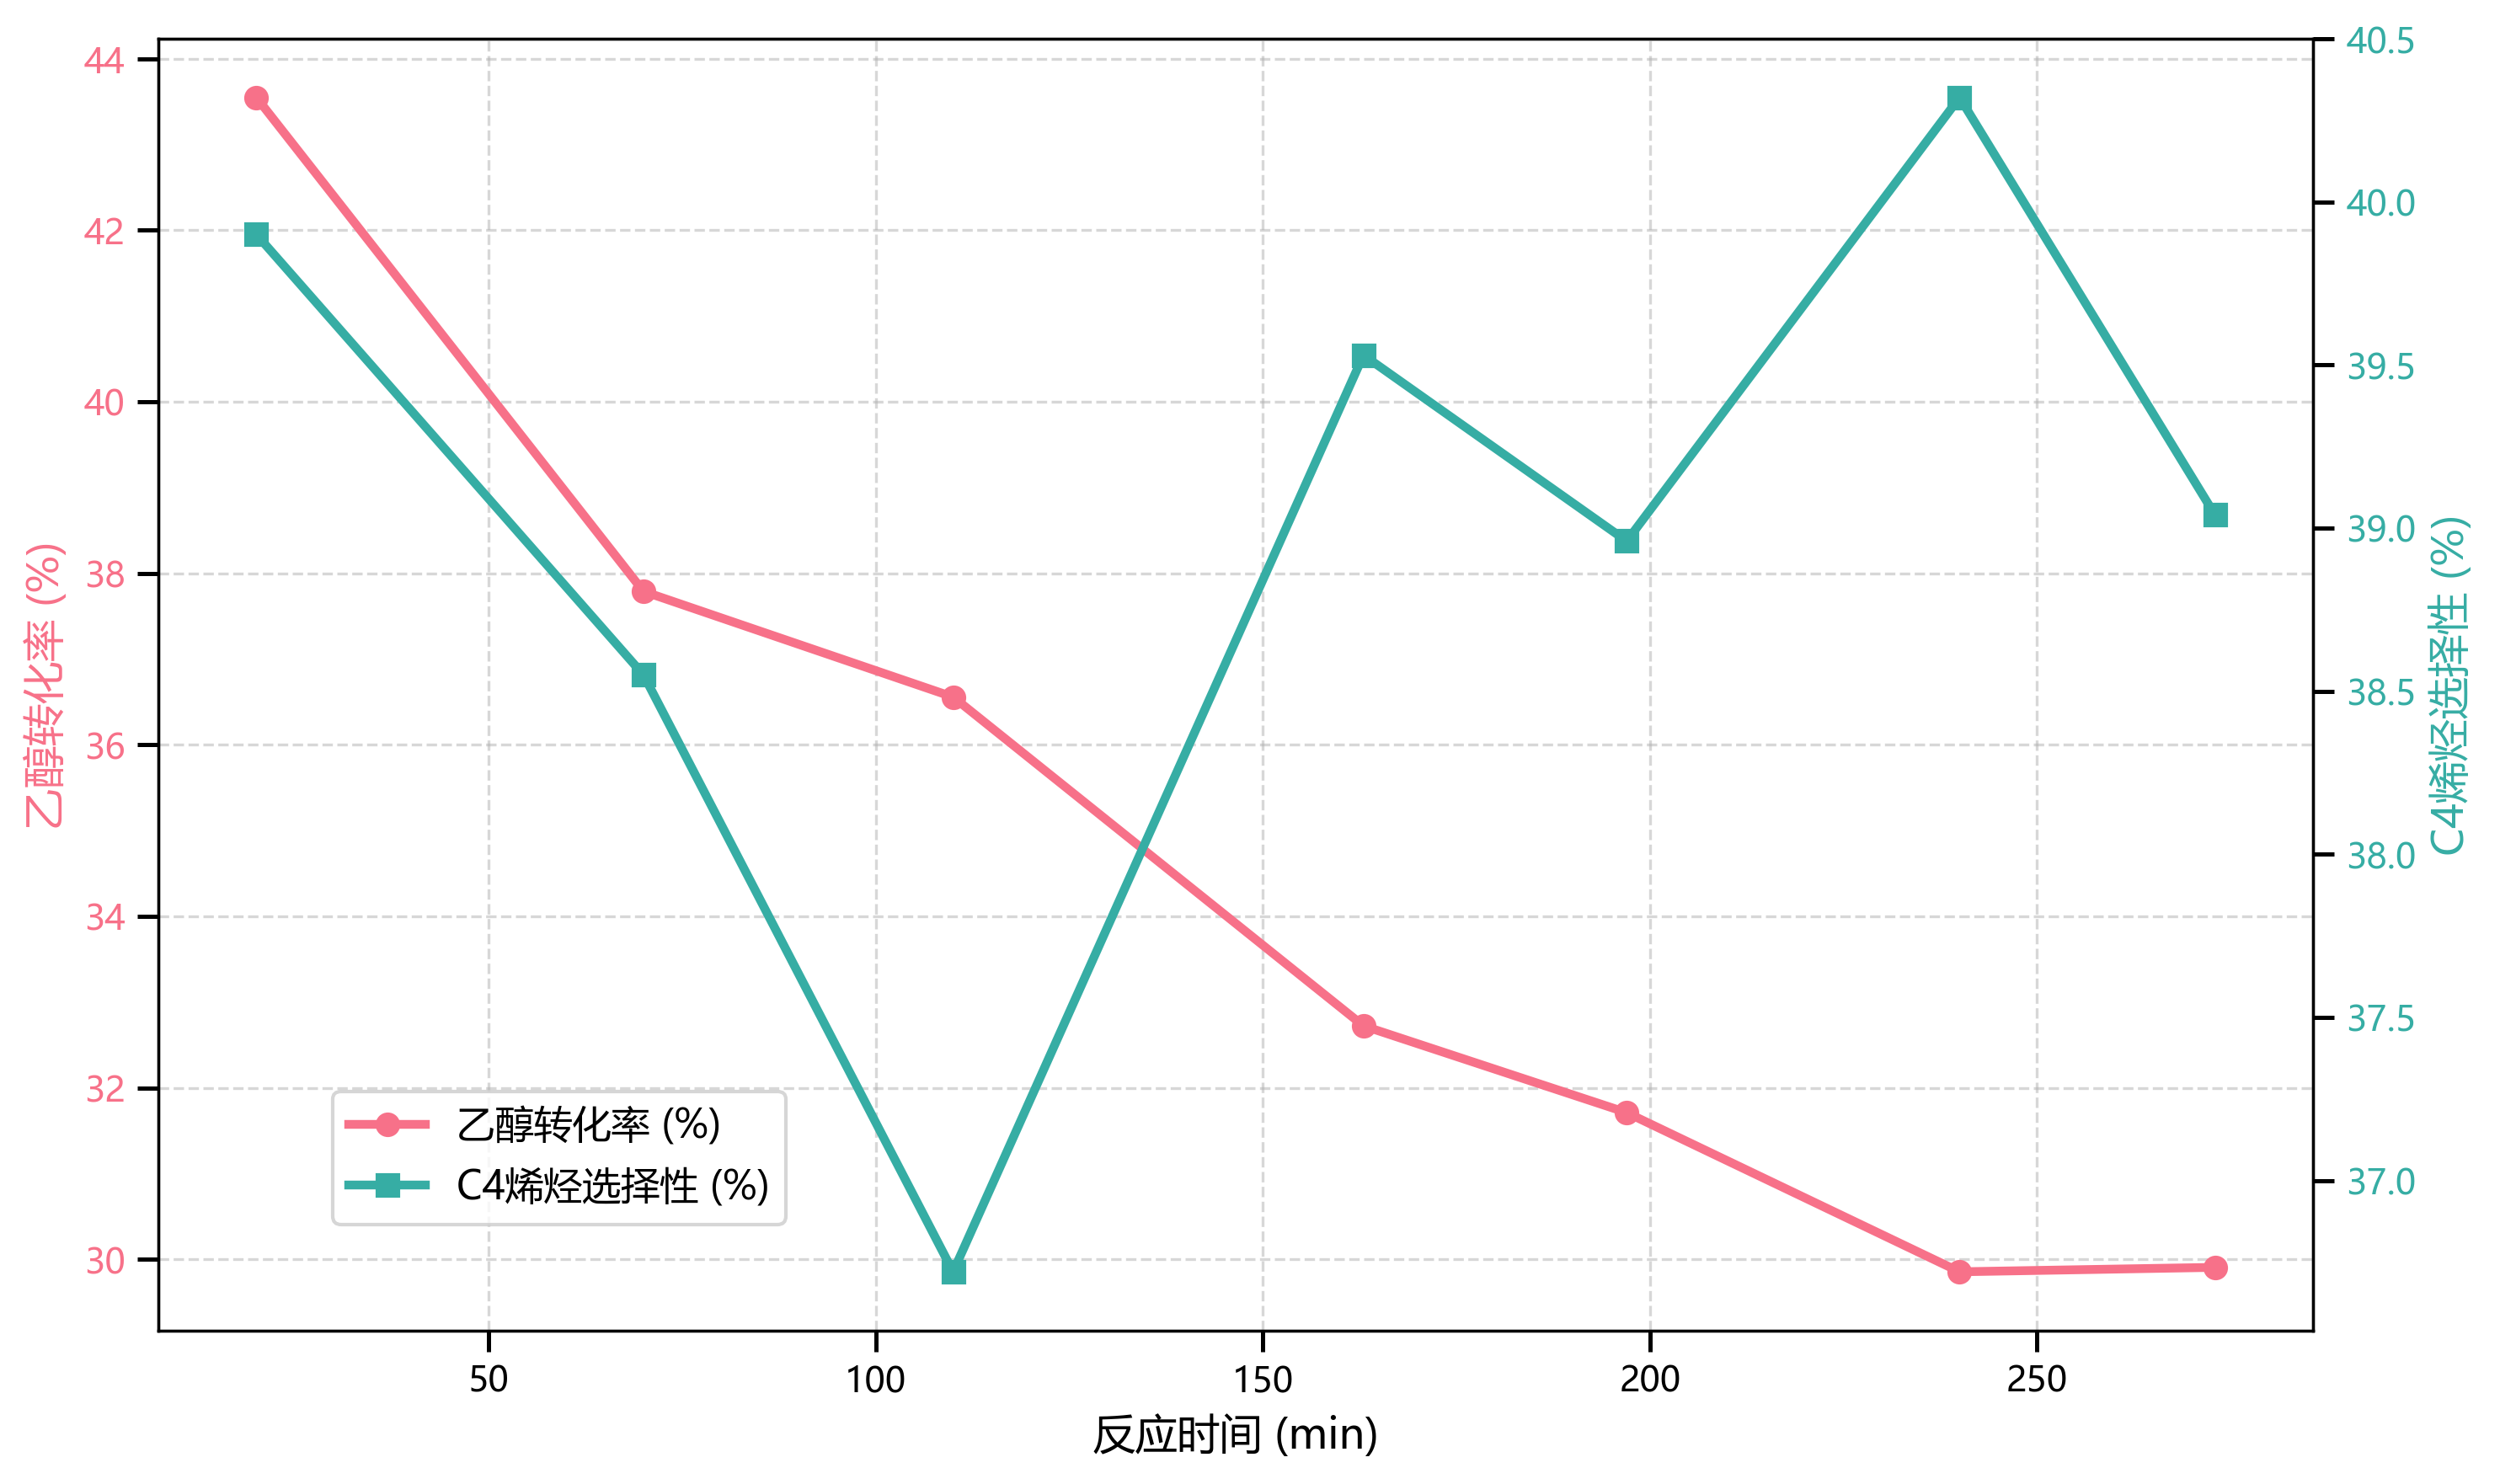
\includegraphics [scale=0.6]{图/1-2-1.png}
	\caption{350°C 下催化剂组合稳定性测试(不同反应时间性能变化)} 
	\label{fig:1}
\end{figure}

\newpage

依照图像,可以发现,随着时间的增加,在一定温度和相同催化剂下,随着时间的增加,反应物乙醇转化率持续下降,逐渐趋于稳定;C4烯烃选择性增加,并趋于稳定,与时间呈现出弱负相关性。20min左右时乙醇转化率为为 43.5\% ,随着时间推移逐渐下降至约 29.9\% (273分钟),表明催化剂可能存在活性衰减或积碳失活现象。同时C4烯烃选择性 在 36.7\% — 40.3\% 之间波动,整体保持相对稳定,说明该催化剂在目标产物选择性上具有较好的抗衰减能力。综合来看,该条件下此催化剂组合在50min内性能较佳,之后效率明显下降,在实际生产中如果在当前条件下进行生产,应当考虑周期性更换催化剂以及控制反应时长等方案。


\subsection{问题二的模型建立与求解}
\subsubsection{控制变量法}
本题要求探究不同组合和温度下反应物转化率和产物选择性的影响,我们考虑通过控制变量法探究催化剂组合和温度中不同变量发生变化的影响,通过对附件一所给数据观察,我们选取了以下组进行不同对照实验:

\begin{enumerate}
	\item 装料方式不同:A9+B5,A12+B1
	\item 乙醇浓度不同:A1+A3,A2+A5,A7+A8+A9+A12,B1+B5,B2+B7
	\item Co负载量不同:A1+A2+A4+A6,A9+A10
	\item 有无HAP:A11+A12
	\item 总质量不变,Co与HAP质量比不同:A12+A13+A14
	\item Co与HAP质量比1:1,总质量不同:B1+B2+B3+B4+B6,A1+A12
\end{enumerate}

\subsubsection{对照实验}
\paragraph{装料方式不同}

原始题目中的名词解释与附件说明中提到A组与B组为两种不同装料方式,这里首先将不同装料方式定为变量控制其余不变,绘制A9组和B5组以及A12组和B1组的对照实验,首先观察A9组和B5组对照结果,影响可视化折线图如图4-5:

\begin{figure}[h]%[h]:固定作用
	\centering%置中
	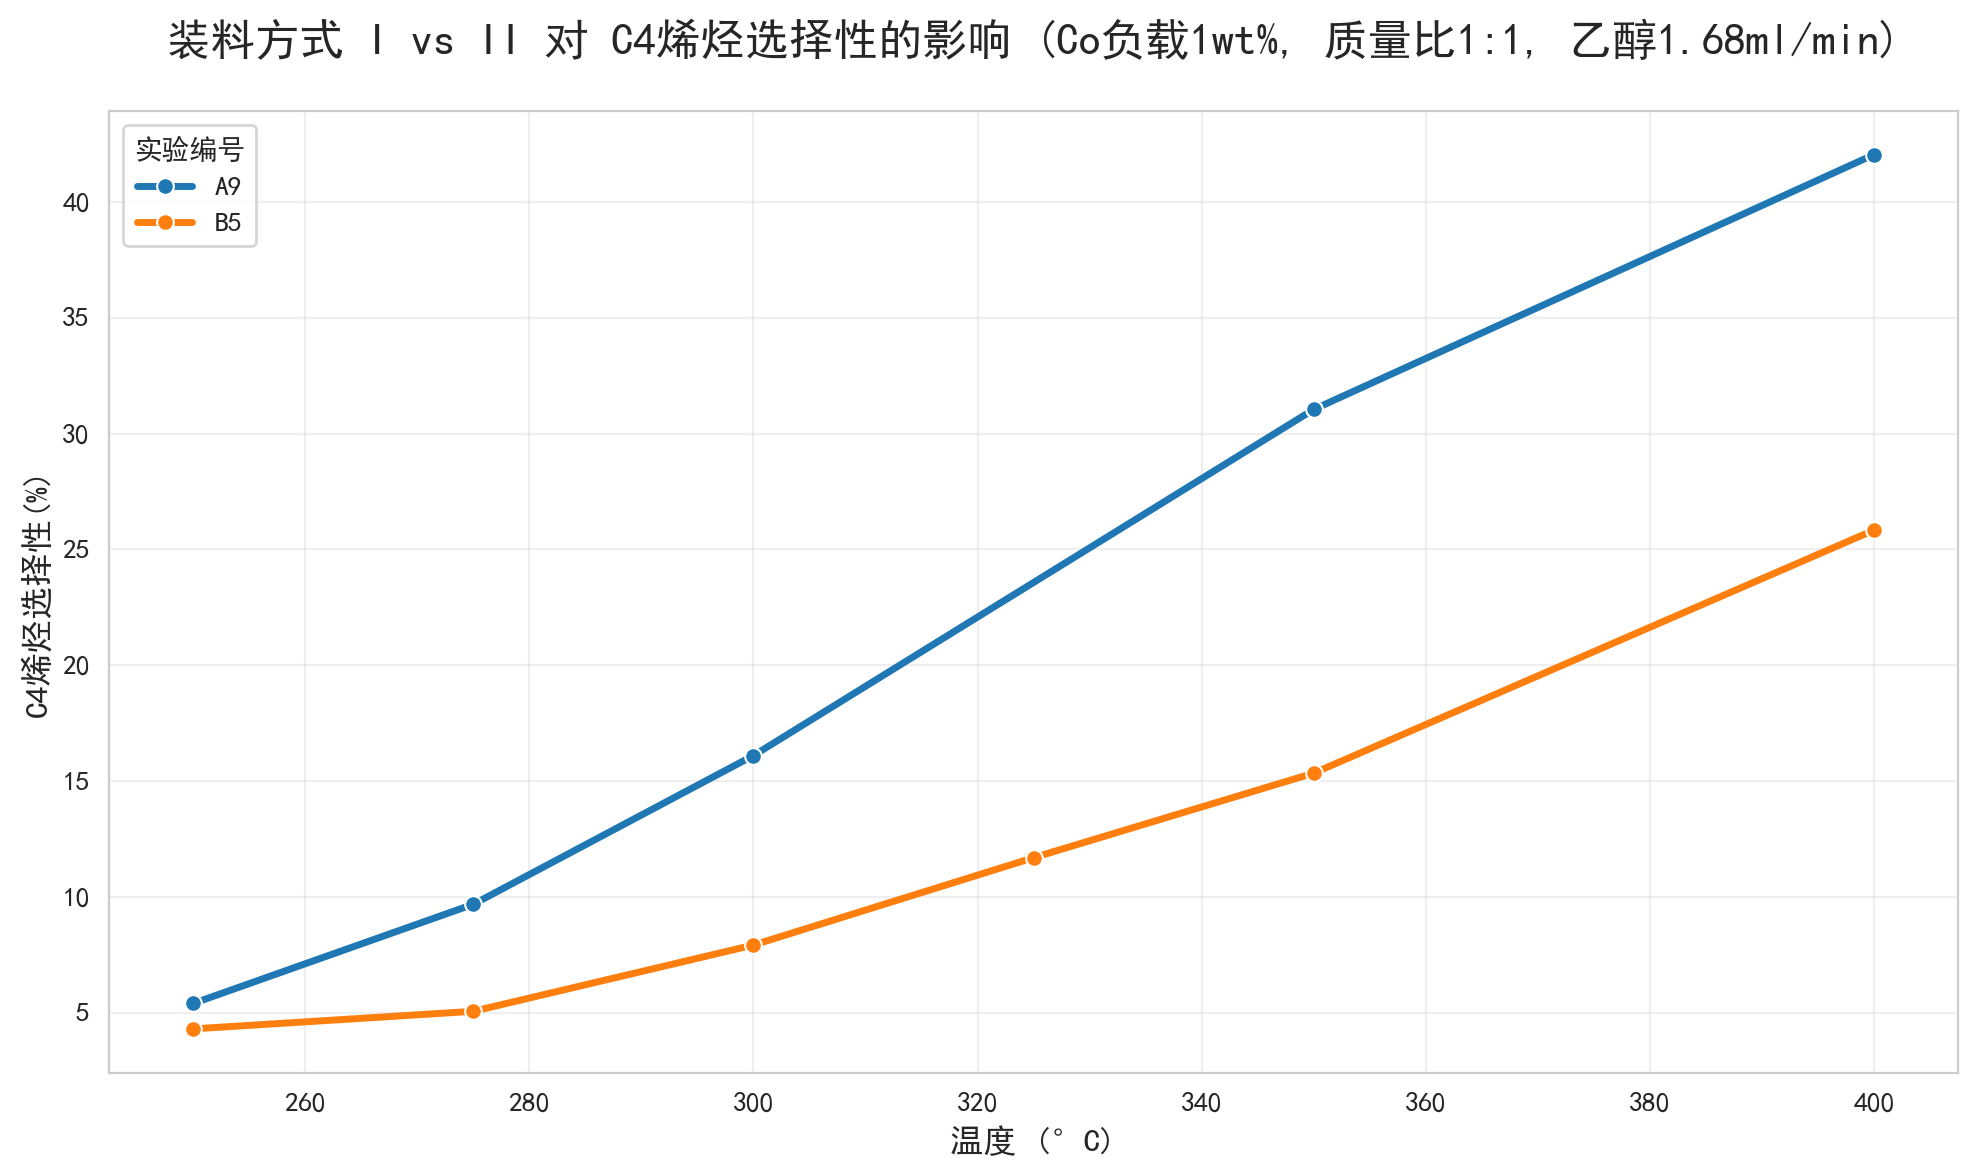
\includegraphics [scale=0.6]{图/2-1-2-1.png}
	\caption{装料方式对C4烯烃选择性的影响(Co负载1wt\%,质量比1:1,乙醇1.68ml/min)} 
	\label{fig:1}
\end{figure}

\begin{figure}[h]%[h]:固定作用
	\centering%置中
	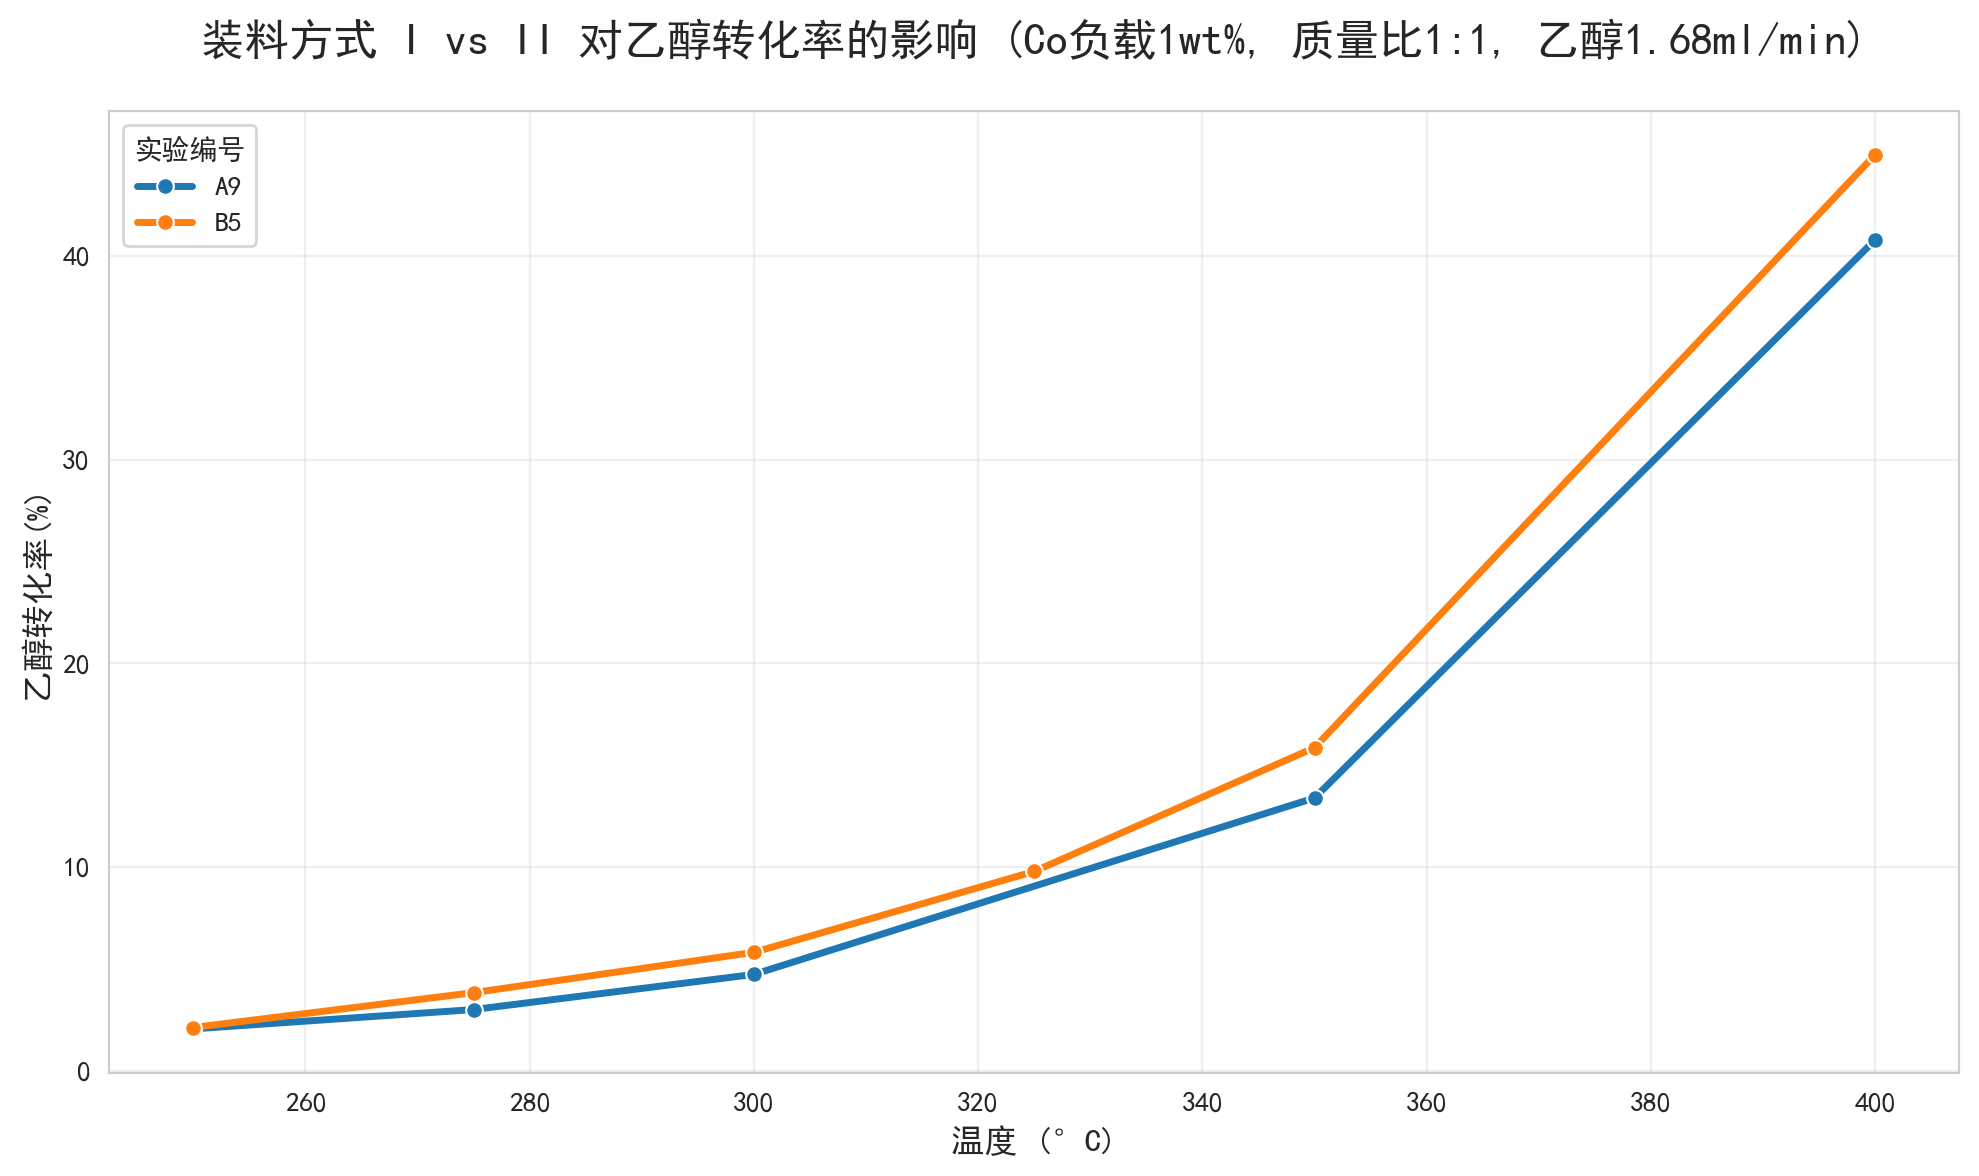
\includegraphics [scale=0.6]{图/2-1-2-2.png}
	\caption{装料方式对乙醇转化率的影响(Co负载1wt\%, 质量比1:1,乙醇1.68ml/min)} 
	\label{fig:1}
\end{figure}

在400°C时,使用B组的装料方式使乙醇转化率 提高了4.18 个百分点,使 \( \text{C}_4 \) 烯烃选择性降低了 16.21 个百分点。同理来观察A12组和B1组对照结果,影响可视化折线图如图6-7:

\begin{figure}[h]%[h]:固定作用
	\centering%置中
	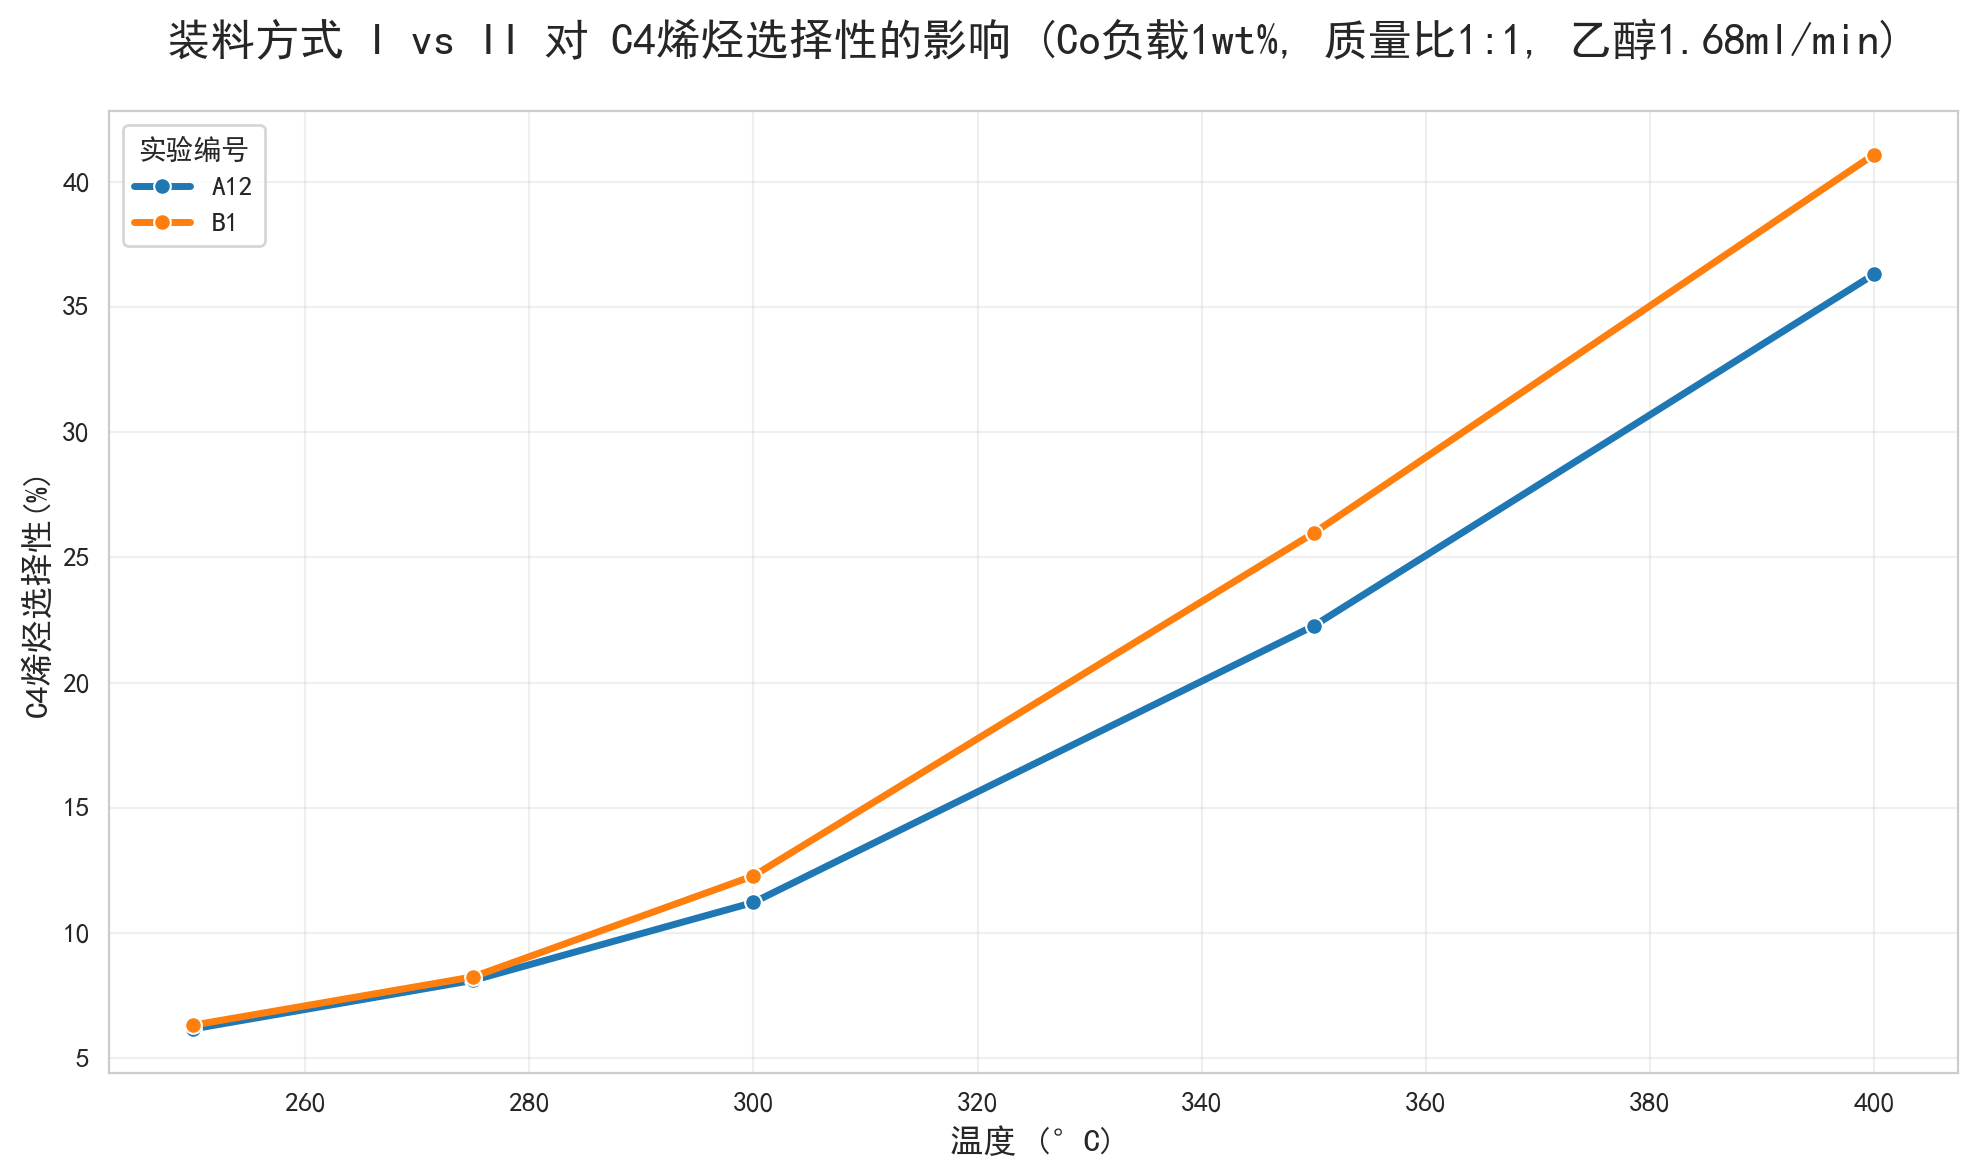
\includegraphics [scale=0.6]{图/2-1-1-1.png}
	\caption{装料方式 I vs II 对 C4烯烃选择性的影响 (Co负载1wt\%, 质量比1:1, 乙醇1.68ml/min)} 
	\label{fig:1}
\end{figure}

\begin{figure}[h]%[h]:固定作用
	\centering%置中
	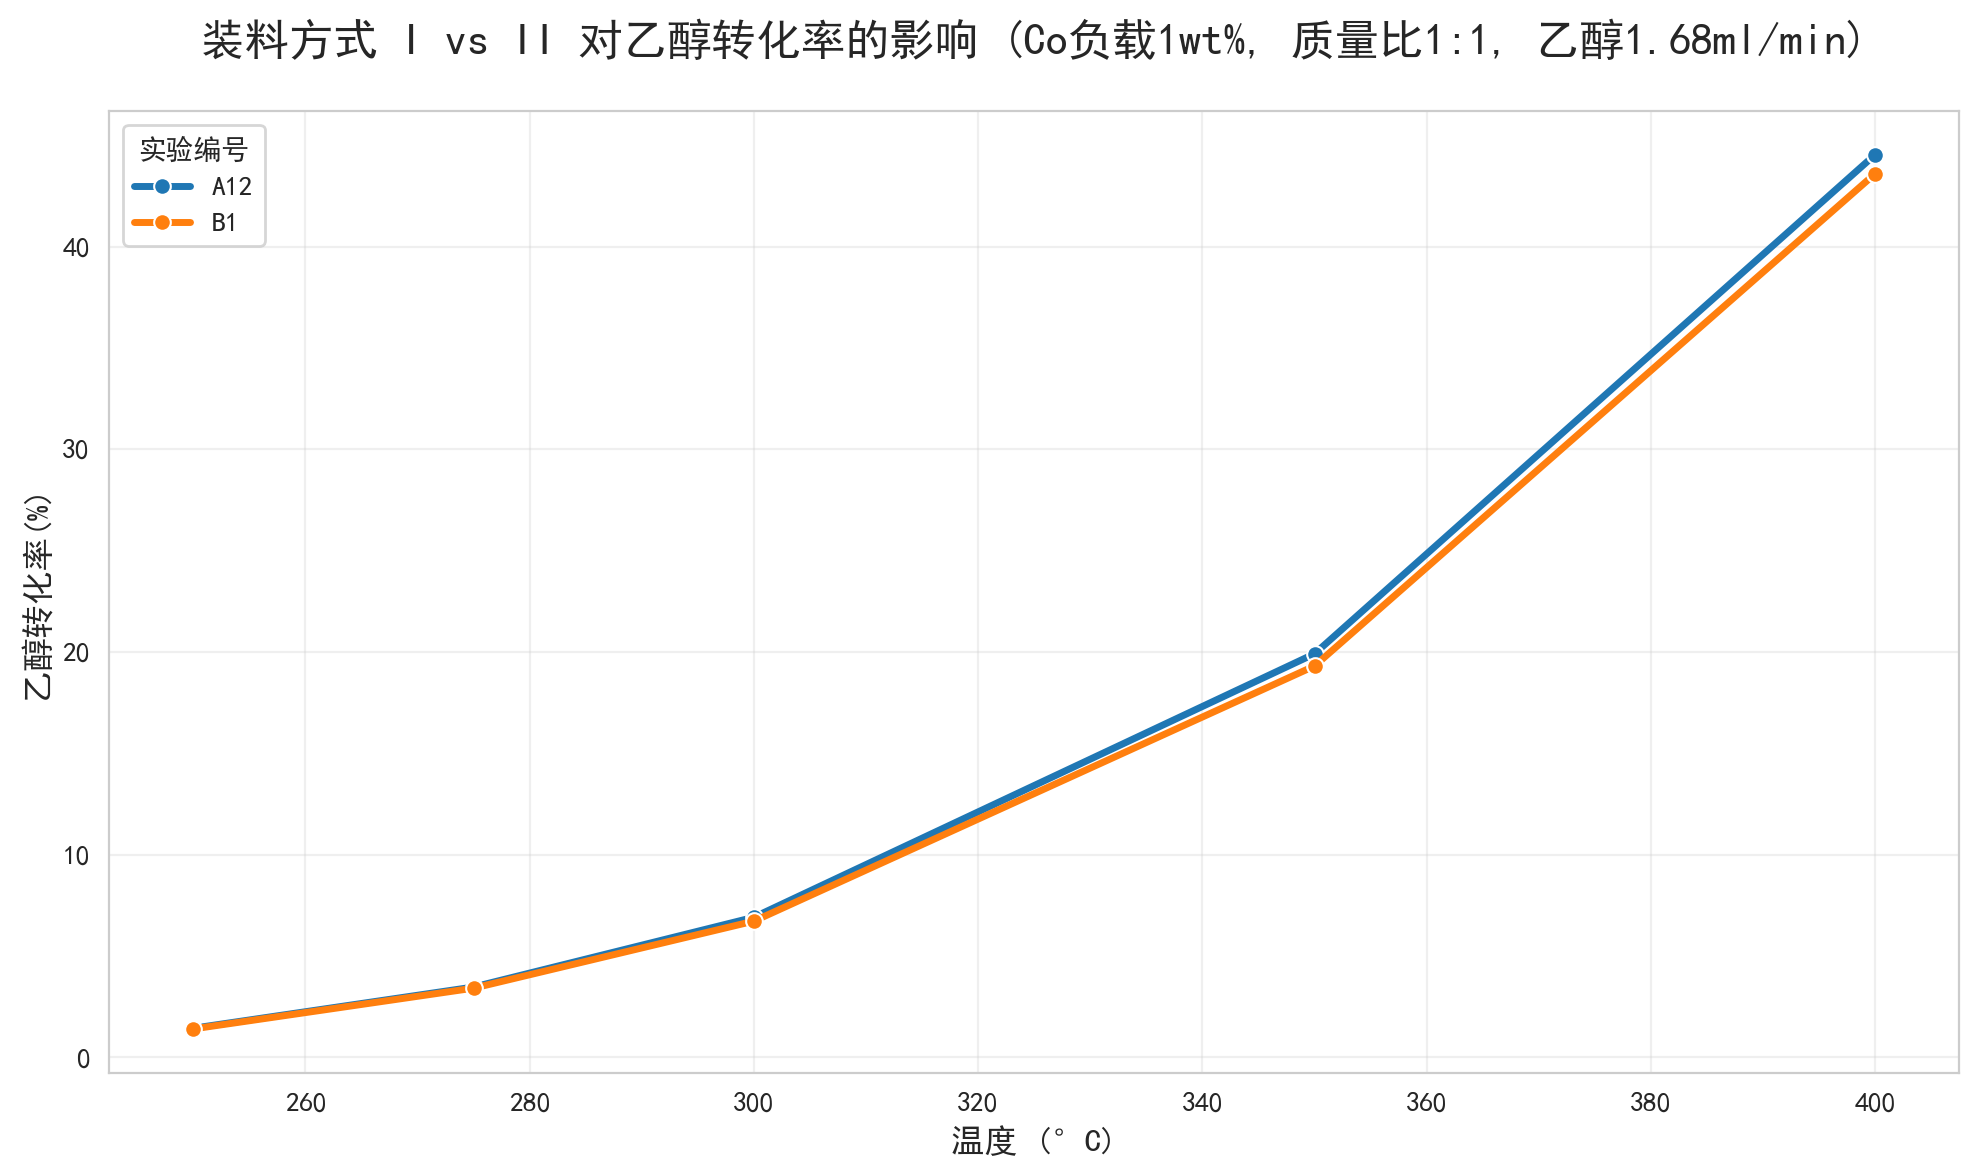
\includegraphics [scale=0.6]{图/2-1-1-2.png}
	\caption{装料方式 I vs II 对乙醇转化率的影响 (Co负载1wt\%, 质量比1:1, 乙醇1.68ml/min)} 
	\label{fig:1}
\end{figure}

在400°C时,使用B组的装料方式使乙醇转化率降低了 0.94 个百分点,使 \( \text{C}_4 \) 烯烃选择性提高了 4.78 个百分点,这与上一组实验所得结论不符,观察两组对照试验之间的差别,主要差异来自乙醇浓度不同如,A9组比A12组乙醇浓度更高,造成的影响需要接下来的对照实验对比乙醇浓度不同来分析结论。

\paragraph{乙醇浓度不同}
乙醇浓度不同组数量庞大,可提供多次不同对照实验,控制其他变量不变,首先观察A1组和A3组的对照结果,影响可视化折线图如图8-9:

\begin{figure}[h]%[h]:固定作用
	\centering%置中
	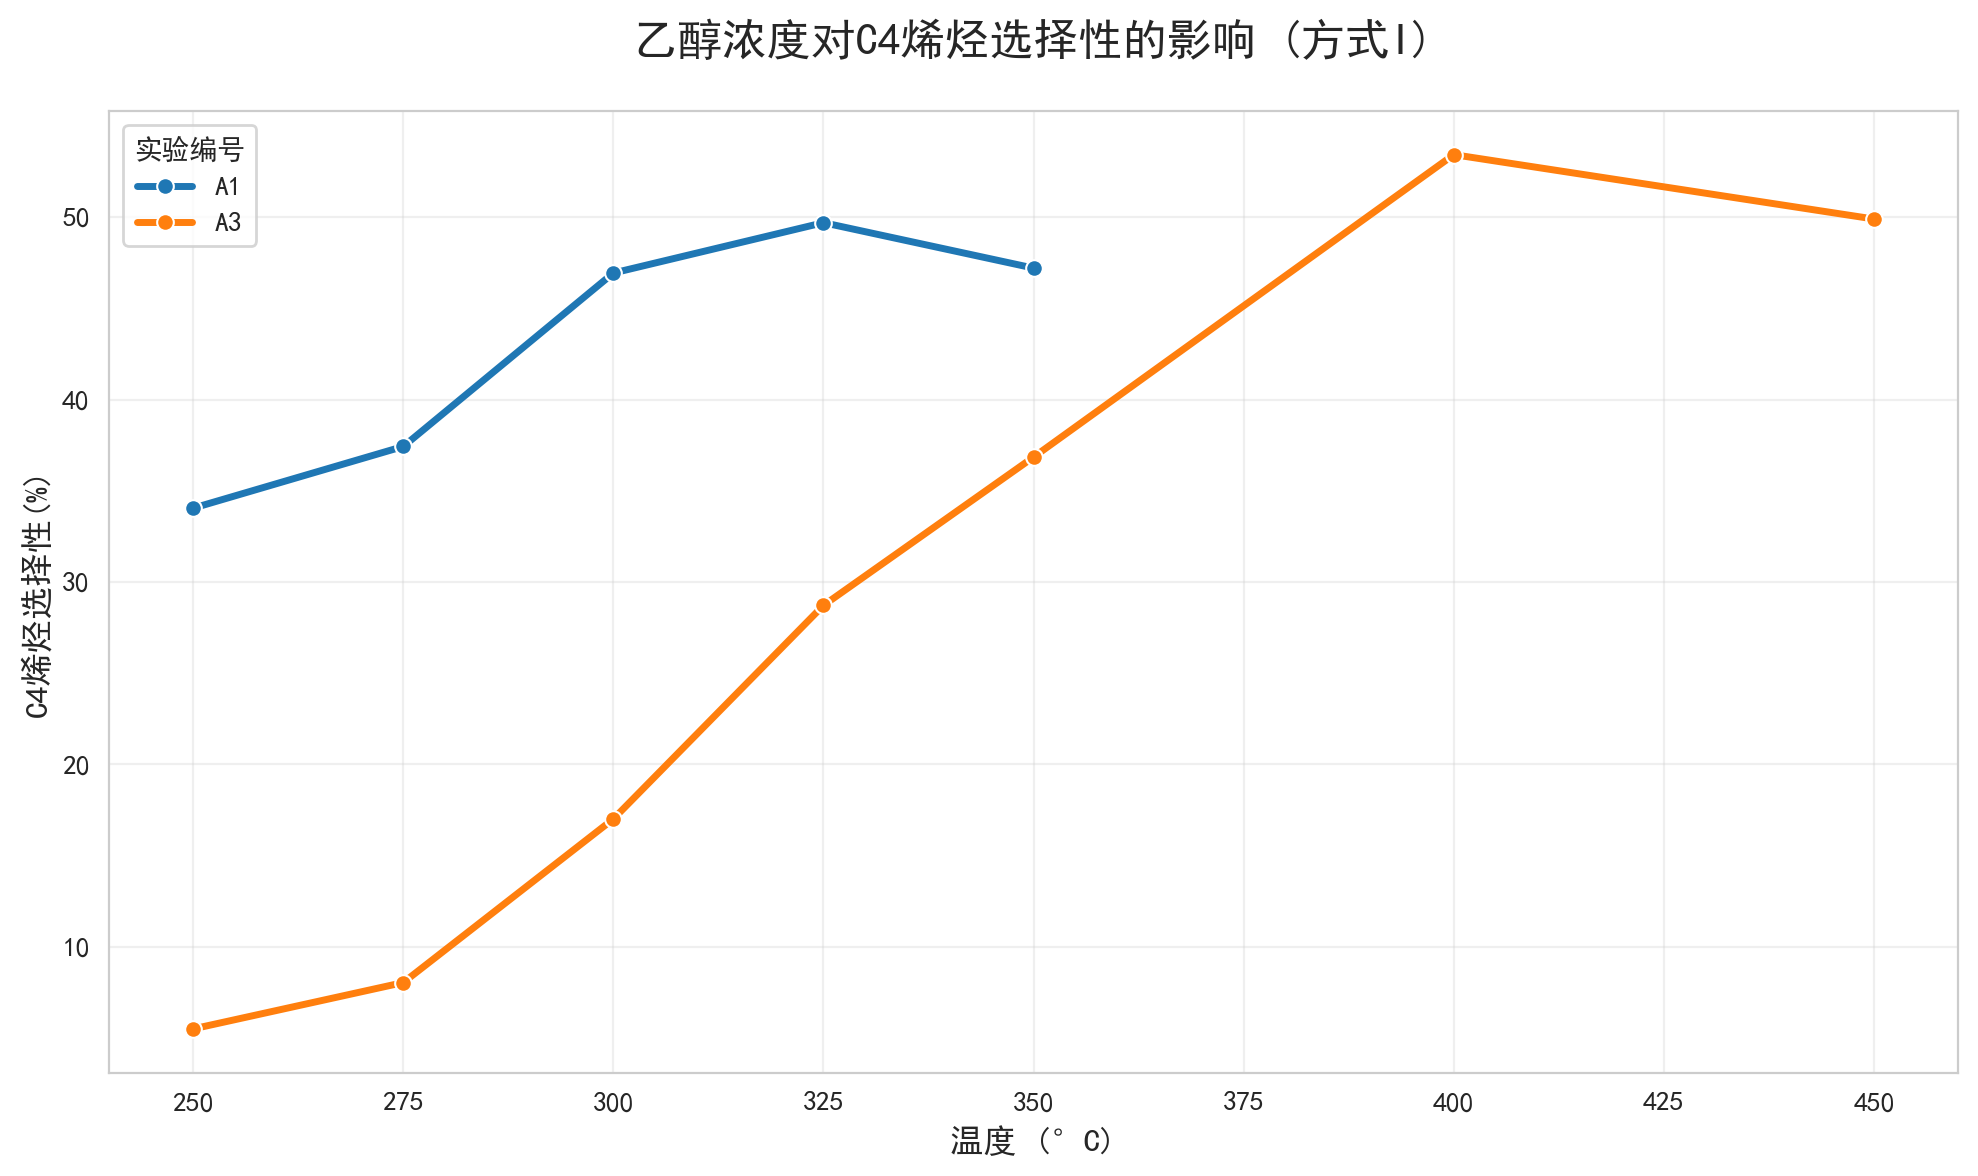
\includegraphics [scale=0.6]{图/2-2-1-1.png}
	\caption{乙醇浓度对C4烯烃选择性的影响 (方式I)} 
	\label{fig:1}
\end{figure}

\newpage

\begin{figure}[h]%[h]:固定作用
	\centering%置中
	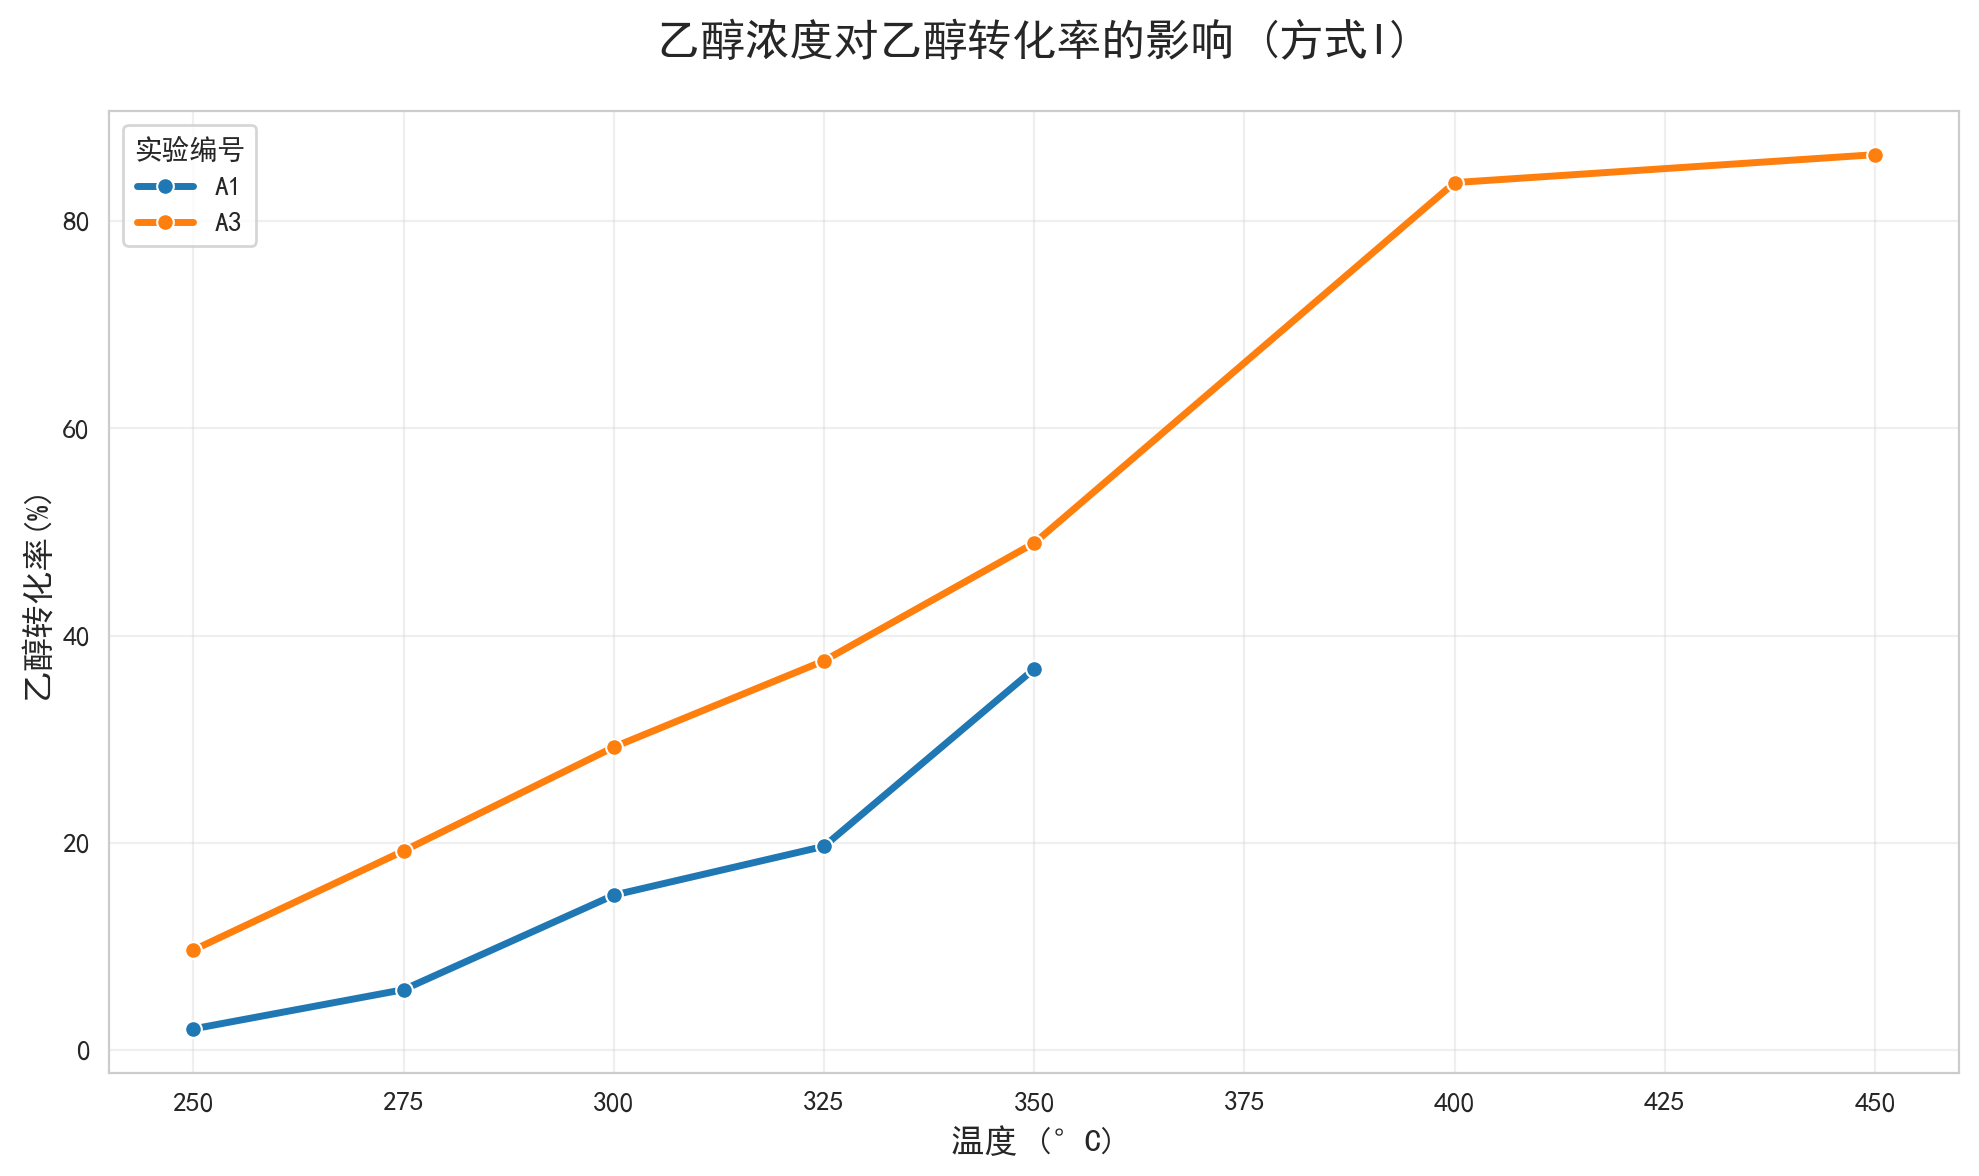
\includegraphics [scale=0.6]{图/2-2-1-2.png}
	\caption{乙醇浓度对乙醇转化率的影响 (方式I)} 
	\label{fig:1}
\end{figure}

其中,A1组乙醇浓度较高(1.68ml/min),A3组乙醇浓度较低(0.9ml/min),从图中可较明显看出高浓度乙醇能提高 \( \text{C}_4 \) 烯烃选择性,但降低乙醇转化率,这与一般化学可逆反应中加反应物可促进正反应进行但反应物转化率会降低相符。接下来观察A2组和A5组的对照结果,影响可视化折线图如图10-11:

\begin{figure}[h]%[h]:固定作用
	\centering%置中
	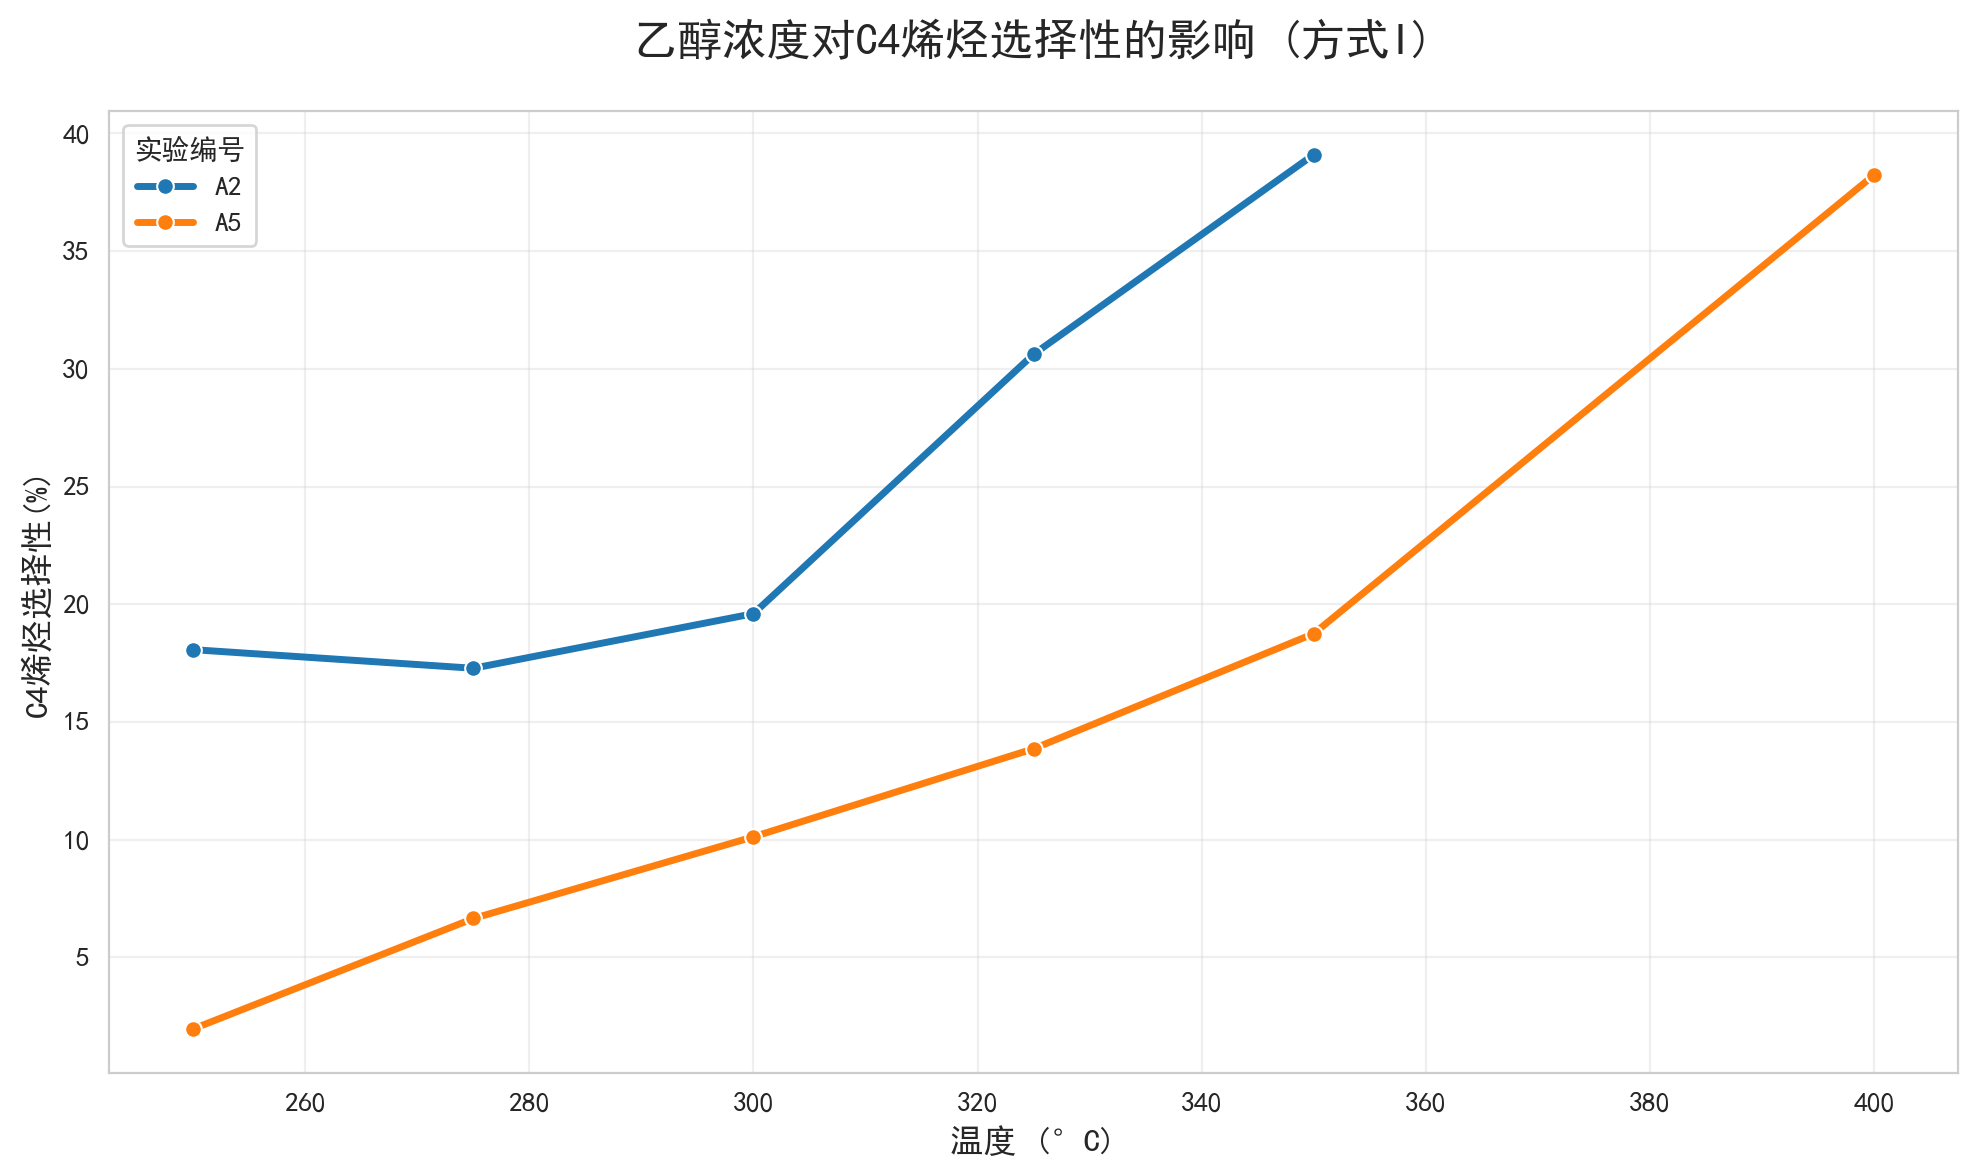
\includegraphics [scale=0.6]{图/2-2-2-1.png}
	\caption{乙醇浓度对C4烯烃选择性的影响 (方式I)} 
	\label{fig:1}
\end{figure}

\begin{figure}[h]%[h]:固定作用
	\centering%置中
	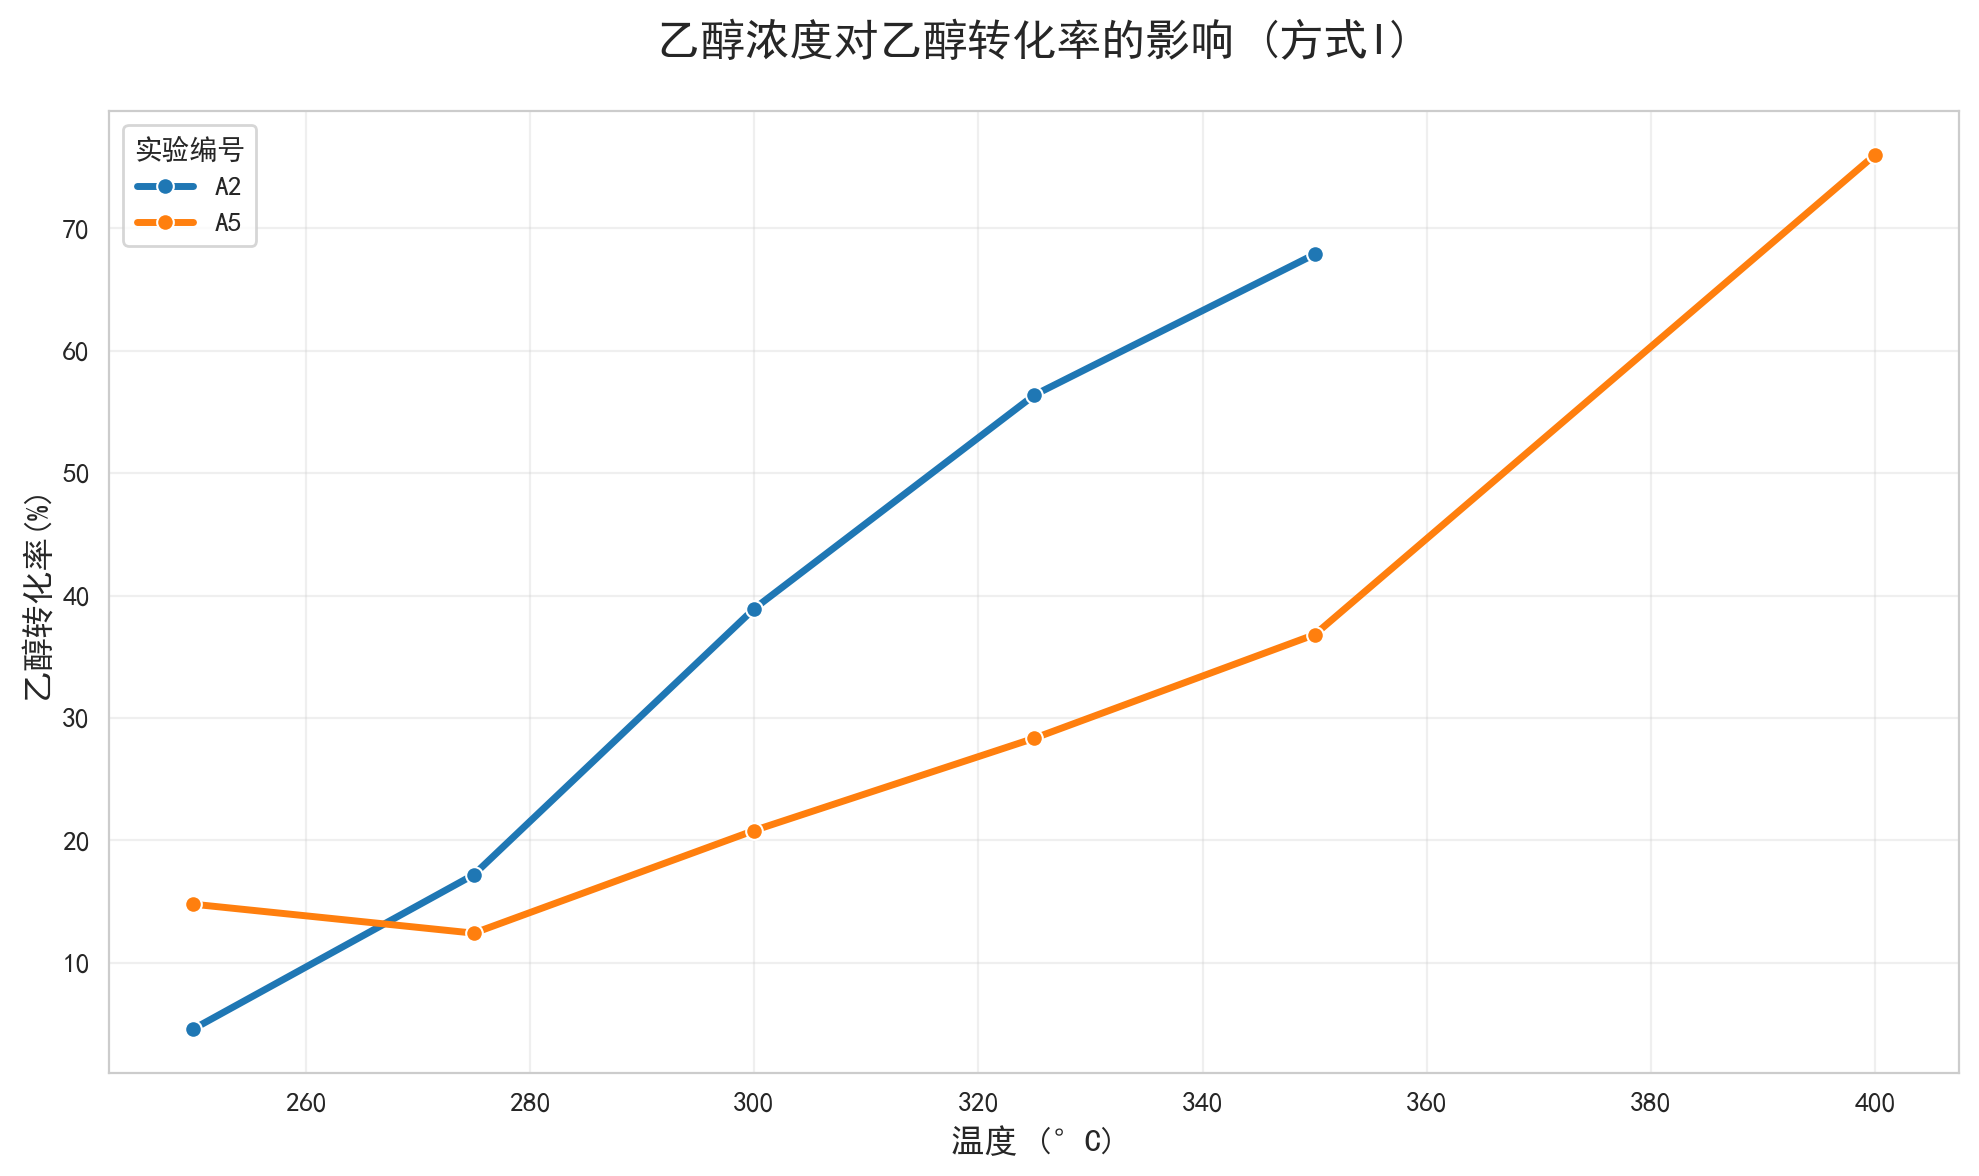
\includegraphics [scale=0.6]{图/2-2-2-2.png}
	\caption{乙醇浓度对乙醇转化率的影响 (方式I)} 
	\label{fig:1}
\end{figure}

其中,A2组乙醇浓度较高(1.68ml/min),A5组乙醇浓度较低(0.3ml/min),这一组的结果与前一组差别在于对乙醇转化率的影响中,随这温度升高,乙醇浓度高的一组乙醇转化率反而更高,这与一般意义上的可逆反应平衡移动不符,推测可能是由于催化剂活性依赖于反应物浓度—即浓度活化效应,某些催化剂需要一定浓度的反应物才能有效激活。我们紧接着观察下一组对照实验A7、A8、A9和A12,可视化结果如图12-13:

\begin{figure}[h]%[h]:固定作用
	\centering%置中
	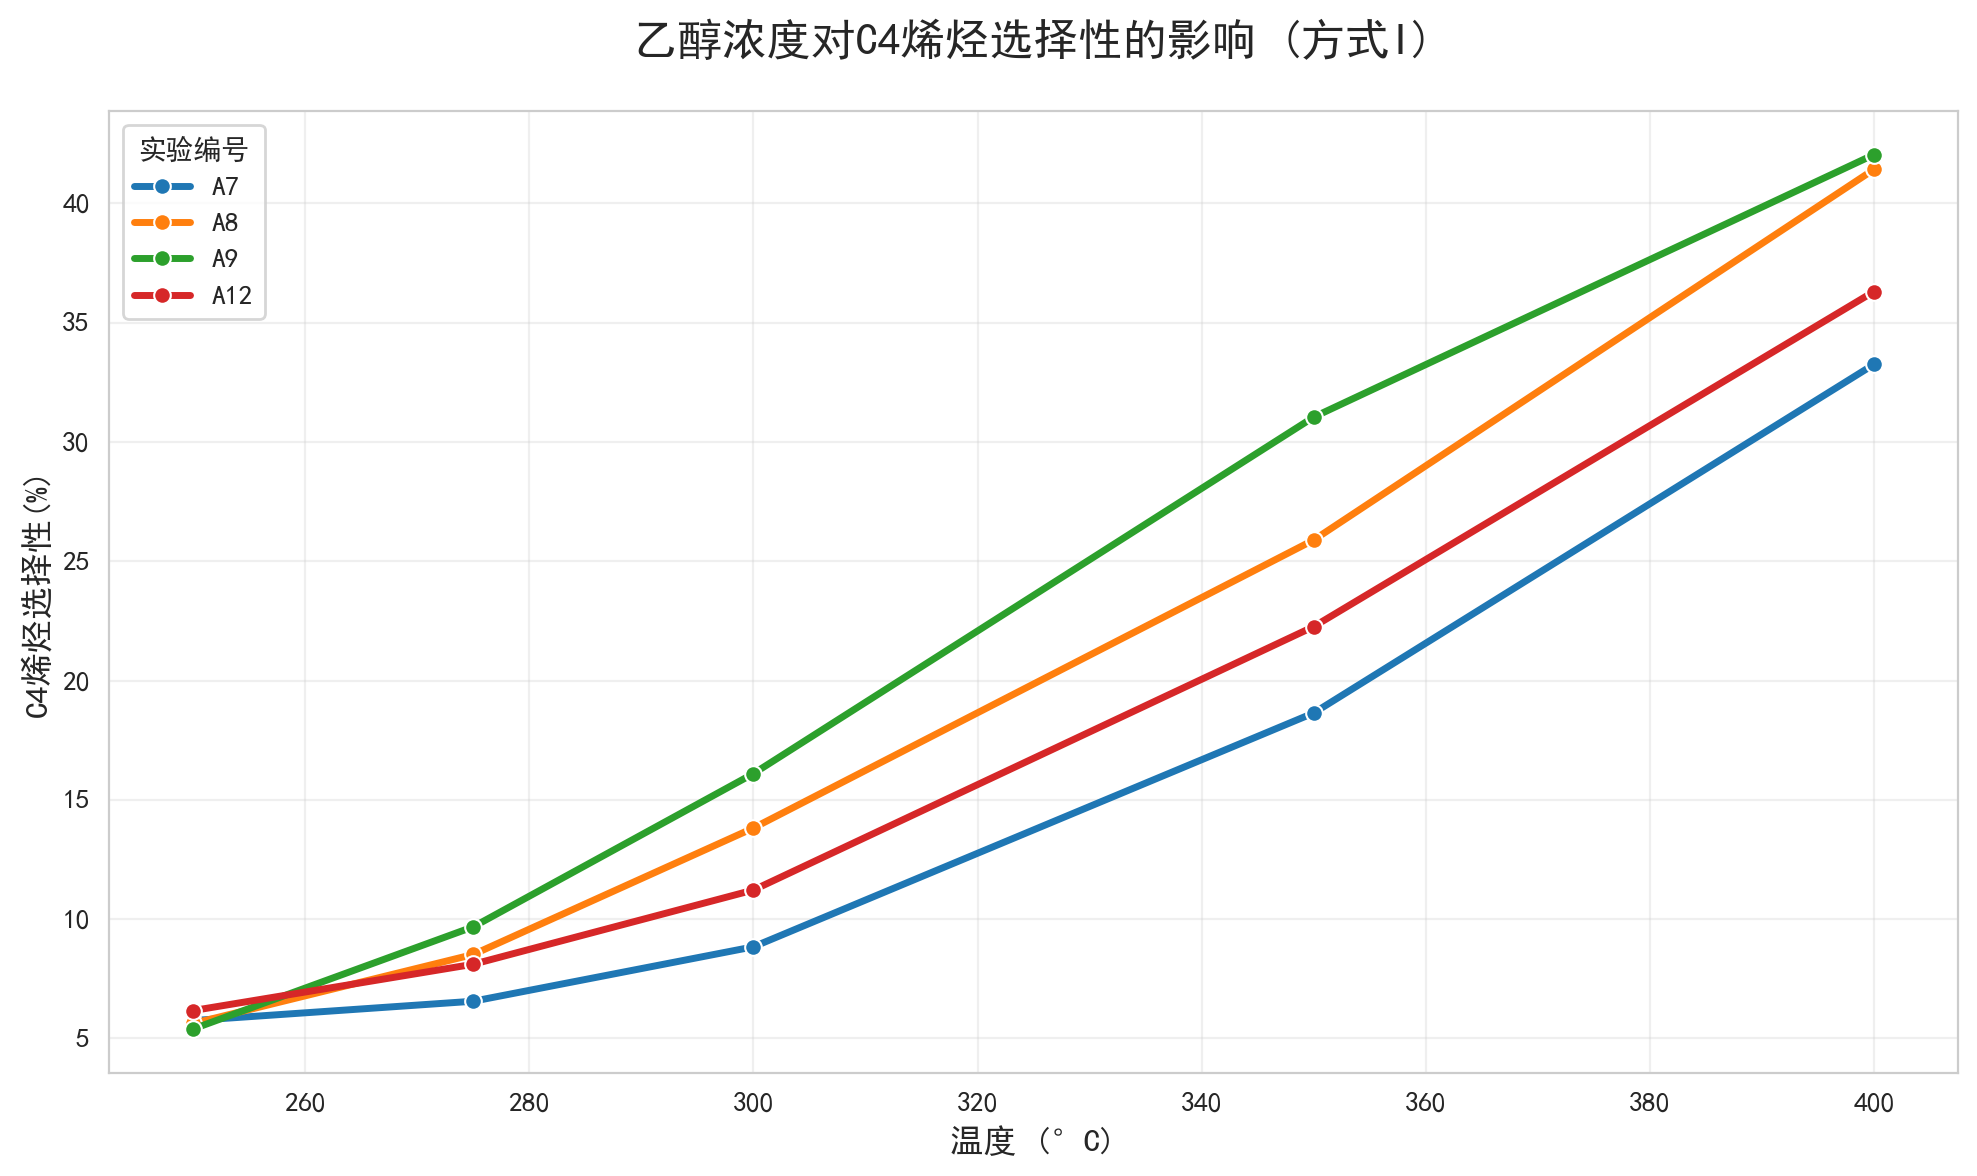
\includegraphics [scale=0.6]{图/2-2-3-1.png}
	\caption{乙醇浓度对C4烯烃选择性的影响 (方式I)} 
	\label{fig:1}
\end{figure}

\begin{figure}[h]%[h]:固定作用
	\centering%置中
	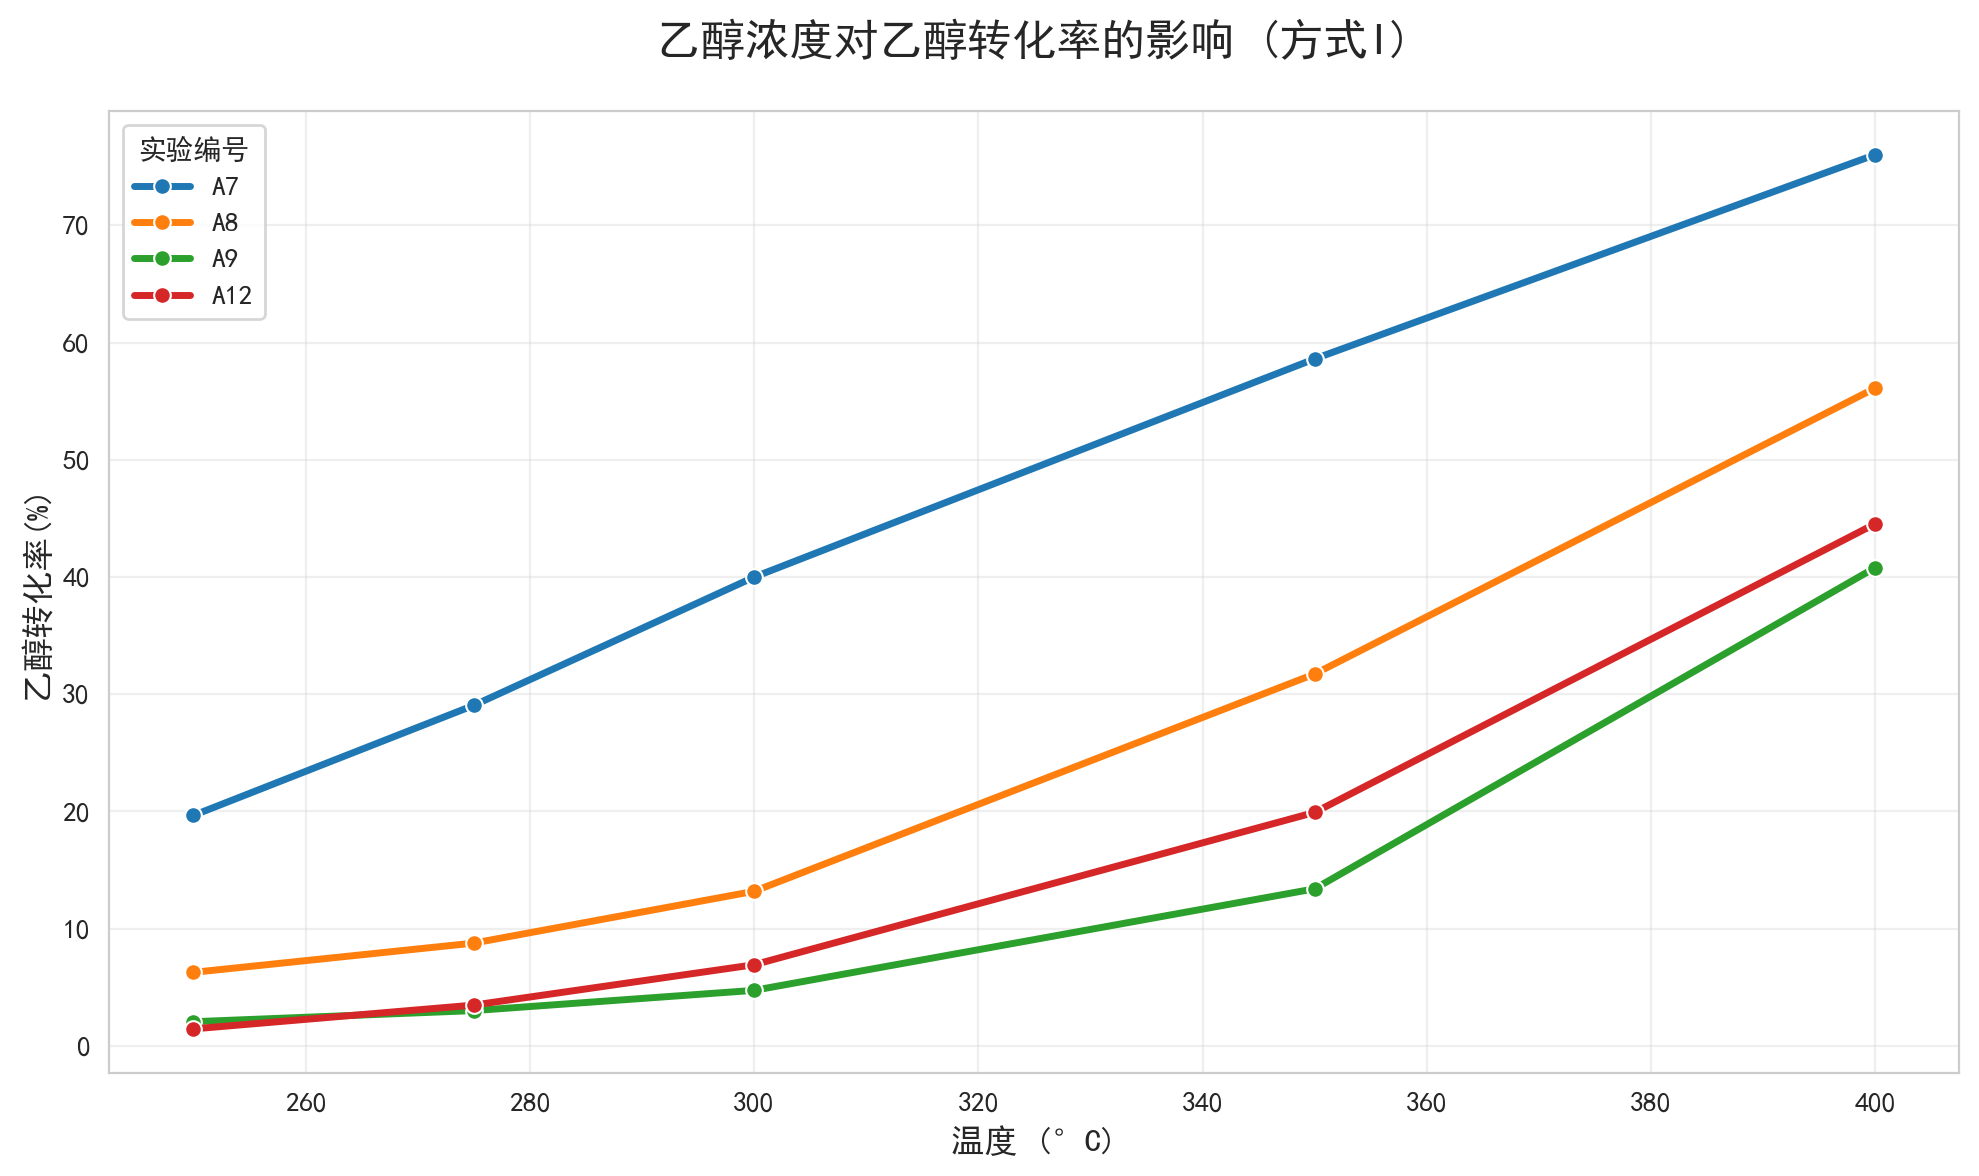
\includegraphics [scale=0.6]{图/2-2-3-2.png}
	\caption{乙醇浓度对乙醇转化率的影响 (方式I)} 
	\label{fig:1}
\end{figure}

这结果中有一处很奇怪,乙醇转化率的图是符合常理的顺序,而 \( \text{C}_4 \) 烯烃选择性的数据中A8和A12位置似乎调换了,按照常理来说A12折线的位置应该位于A8和A9之间,据此推测可能由于增加乙醇浓度过程中副反应竞争加剧,而再增加乙醇浓度的时候主反应进入高效率区,此时副反应饱和。乙醇浓度不同其他对照实验组详细对照图详见附录。





\paragraph{Co负载量不同}
针对不同负载量主要有两组实验,首先观察A9组和A10组,转化率与选择性可视化结果如图14-15:

\newpage

\begin{figure}[h]%[h]:固定作用
	\centering%置中
	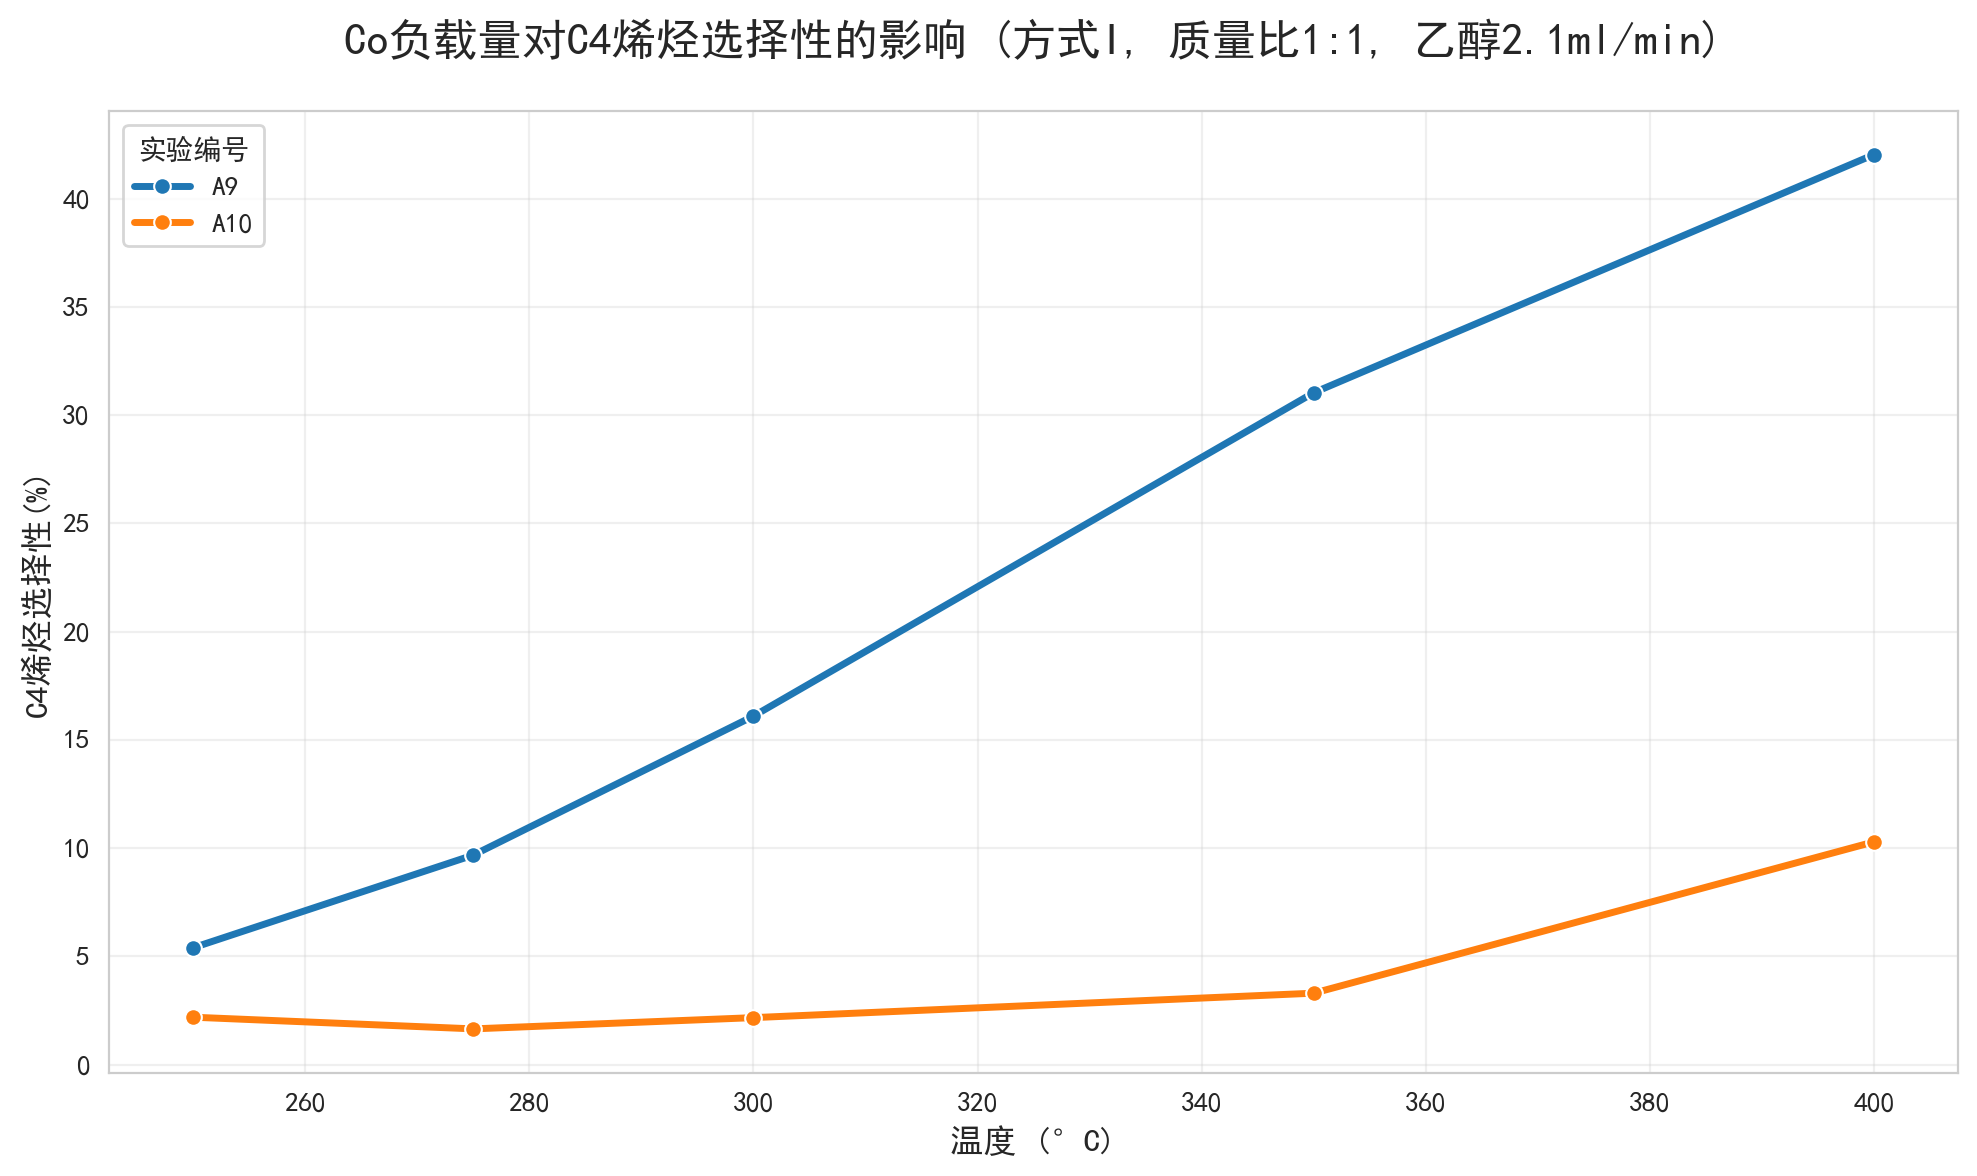
\includegraphics [scale=0.6]{图/2-3-2-1.png}
	\caption{乙醇浓度对C4烯烃选择性的影响 (方式I)} 
	\label{fig:1}
\end{figure}

\begin{figure}[h]%[h]:固定作用
	\centering%置中
	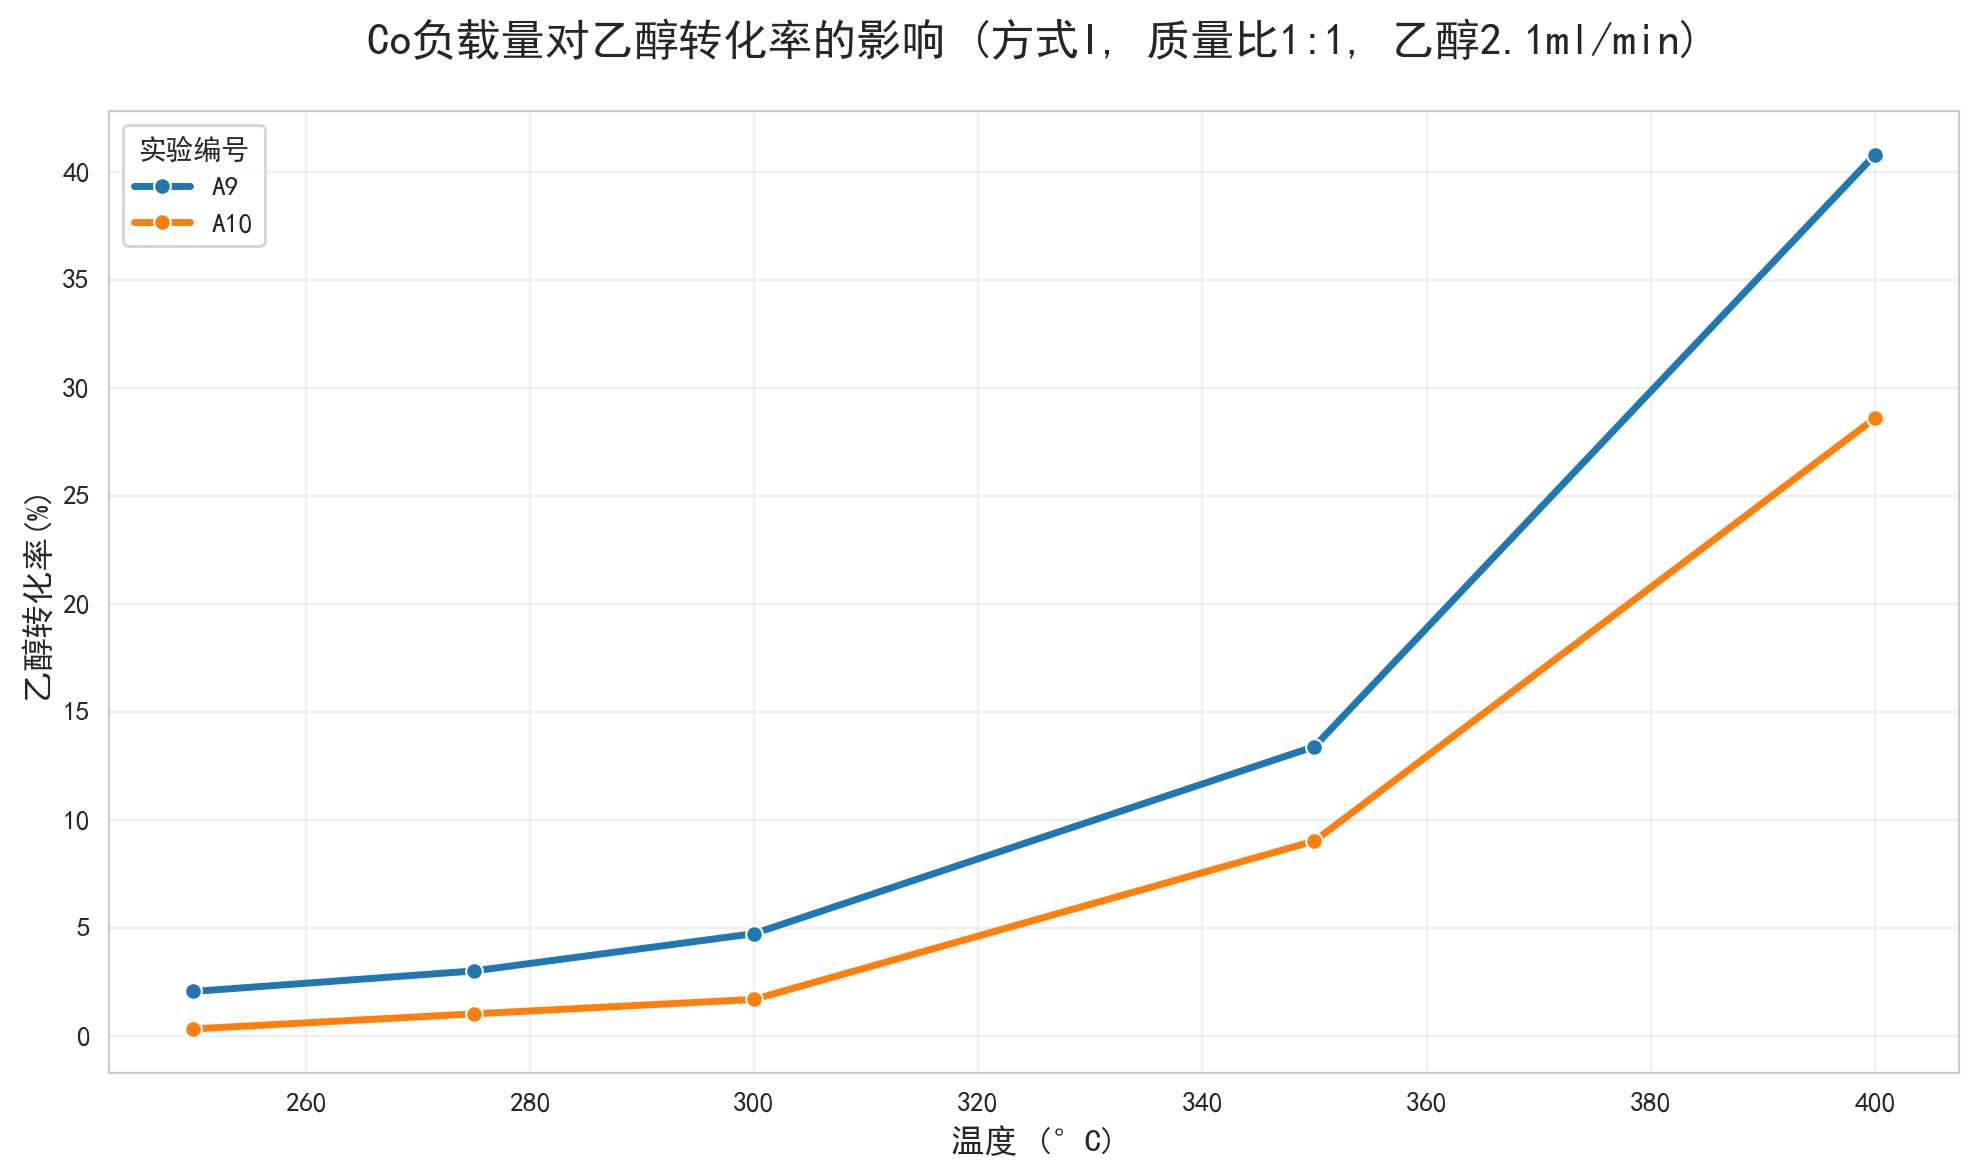
\includegraphics [scale=0.6]{图/2-3-2-2.png}
	\caption{乙醇浓度对乙醇转化率的影响 (方式I)} 
	\label{fig:1}
\end{figure}

提高Co的负载量即降低催化剂相对表面积,相对表面积越大转化率与选择性越高,其他实验组对比结果详细请看附录。


\paragraph{有无HAP}
该组对照较为简单,主要观察HAP是否存在对该反应的影响即可,观察指标就是转化率和选择性是否有变化,绘制图像如图16-17:

\begin{figure}[h]%[h]:固定作用
	\centering%置中
	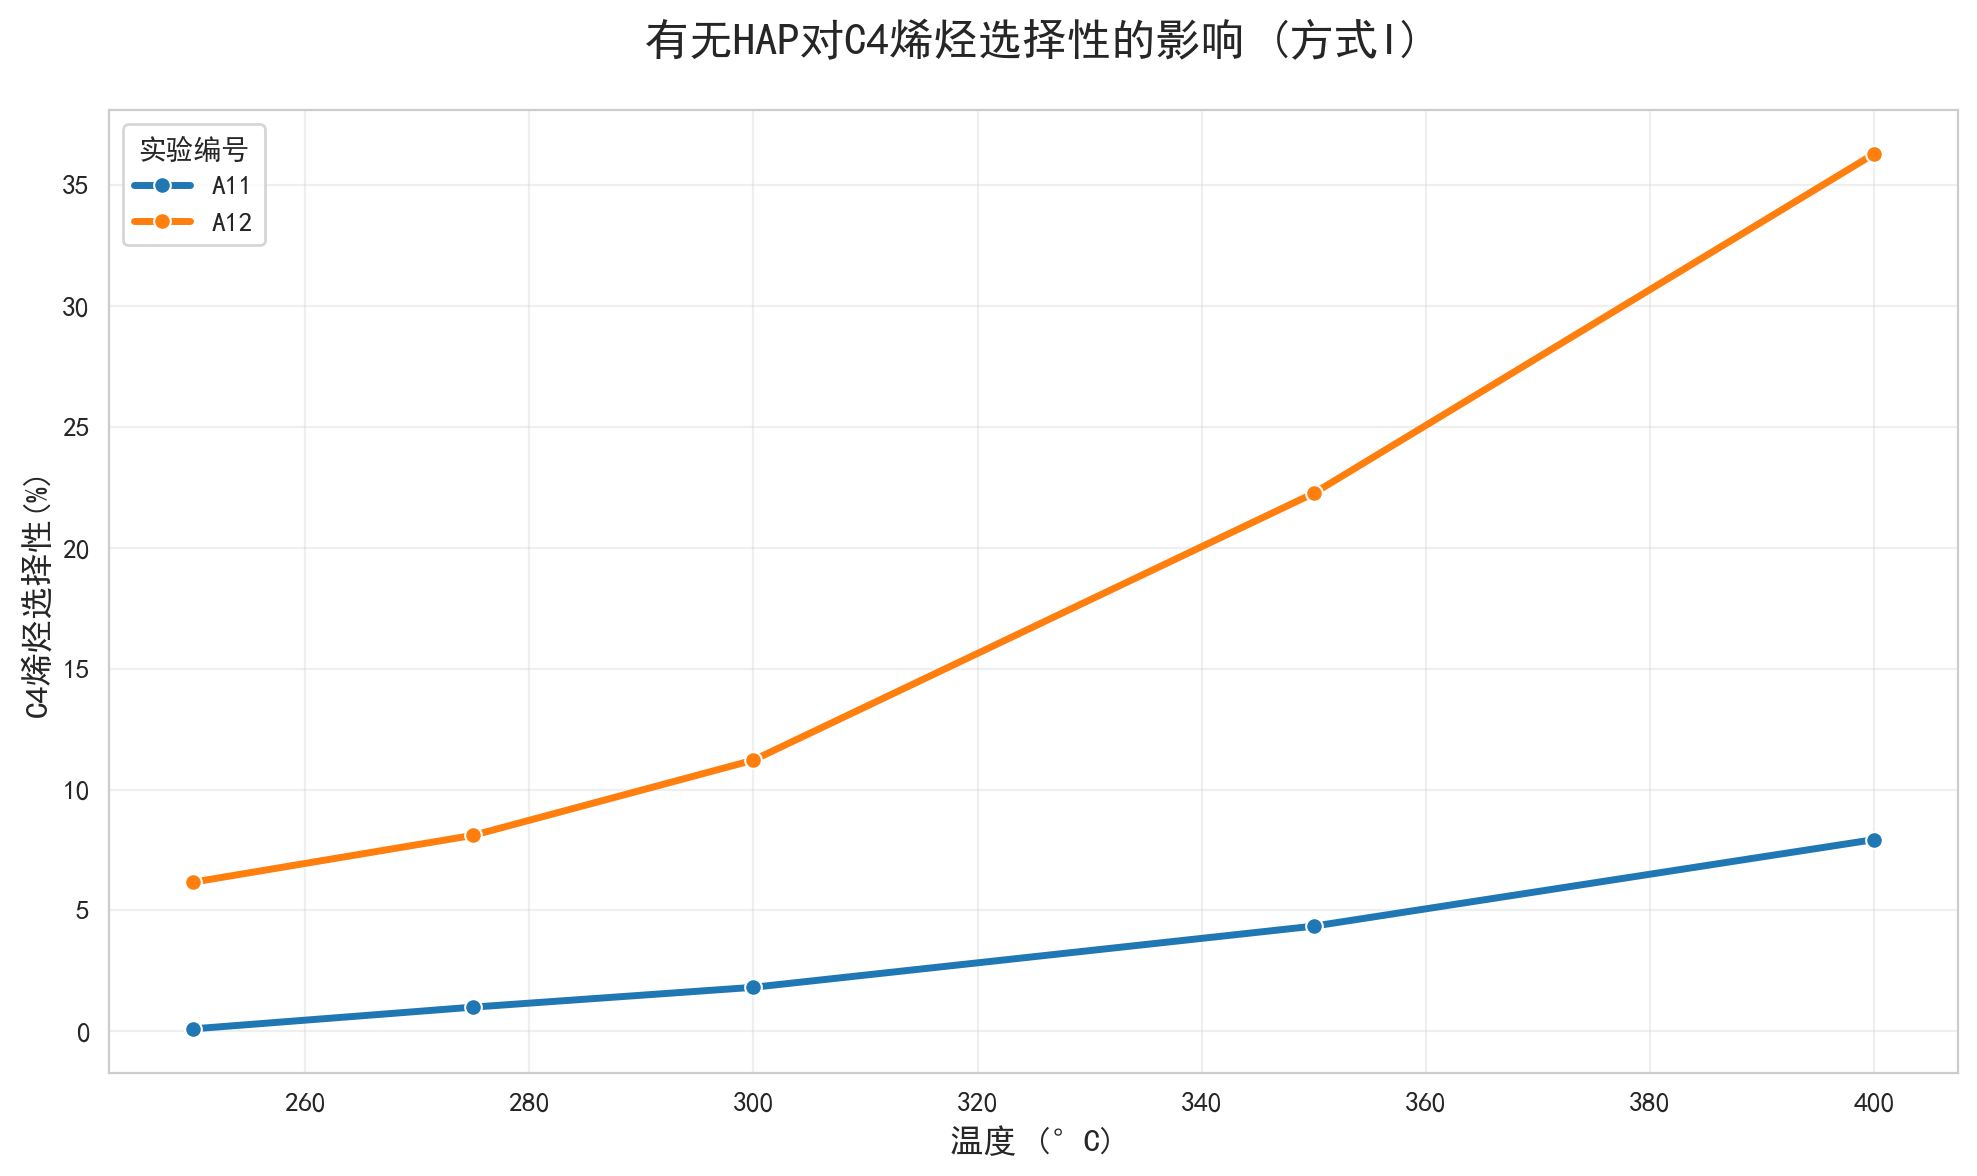
\includegraphics [scale=0.6]{图/2-4-1-1.png}
	\caption{有无HAP对C4烯烃选择性的影响 (方式I)} 
	\label{fig:1}
\end{figure}

\begin{figure}[h]%[h]:固定作用
	\centering%置中
	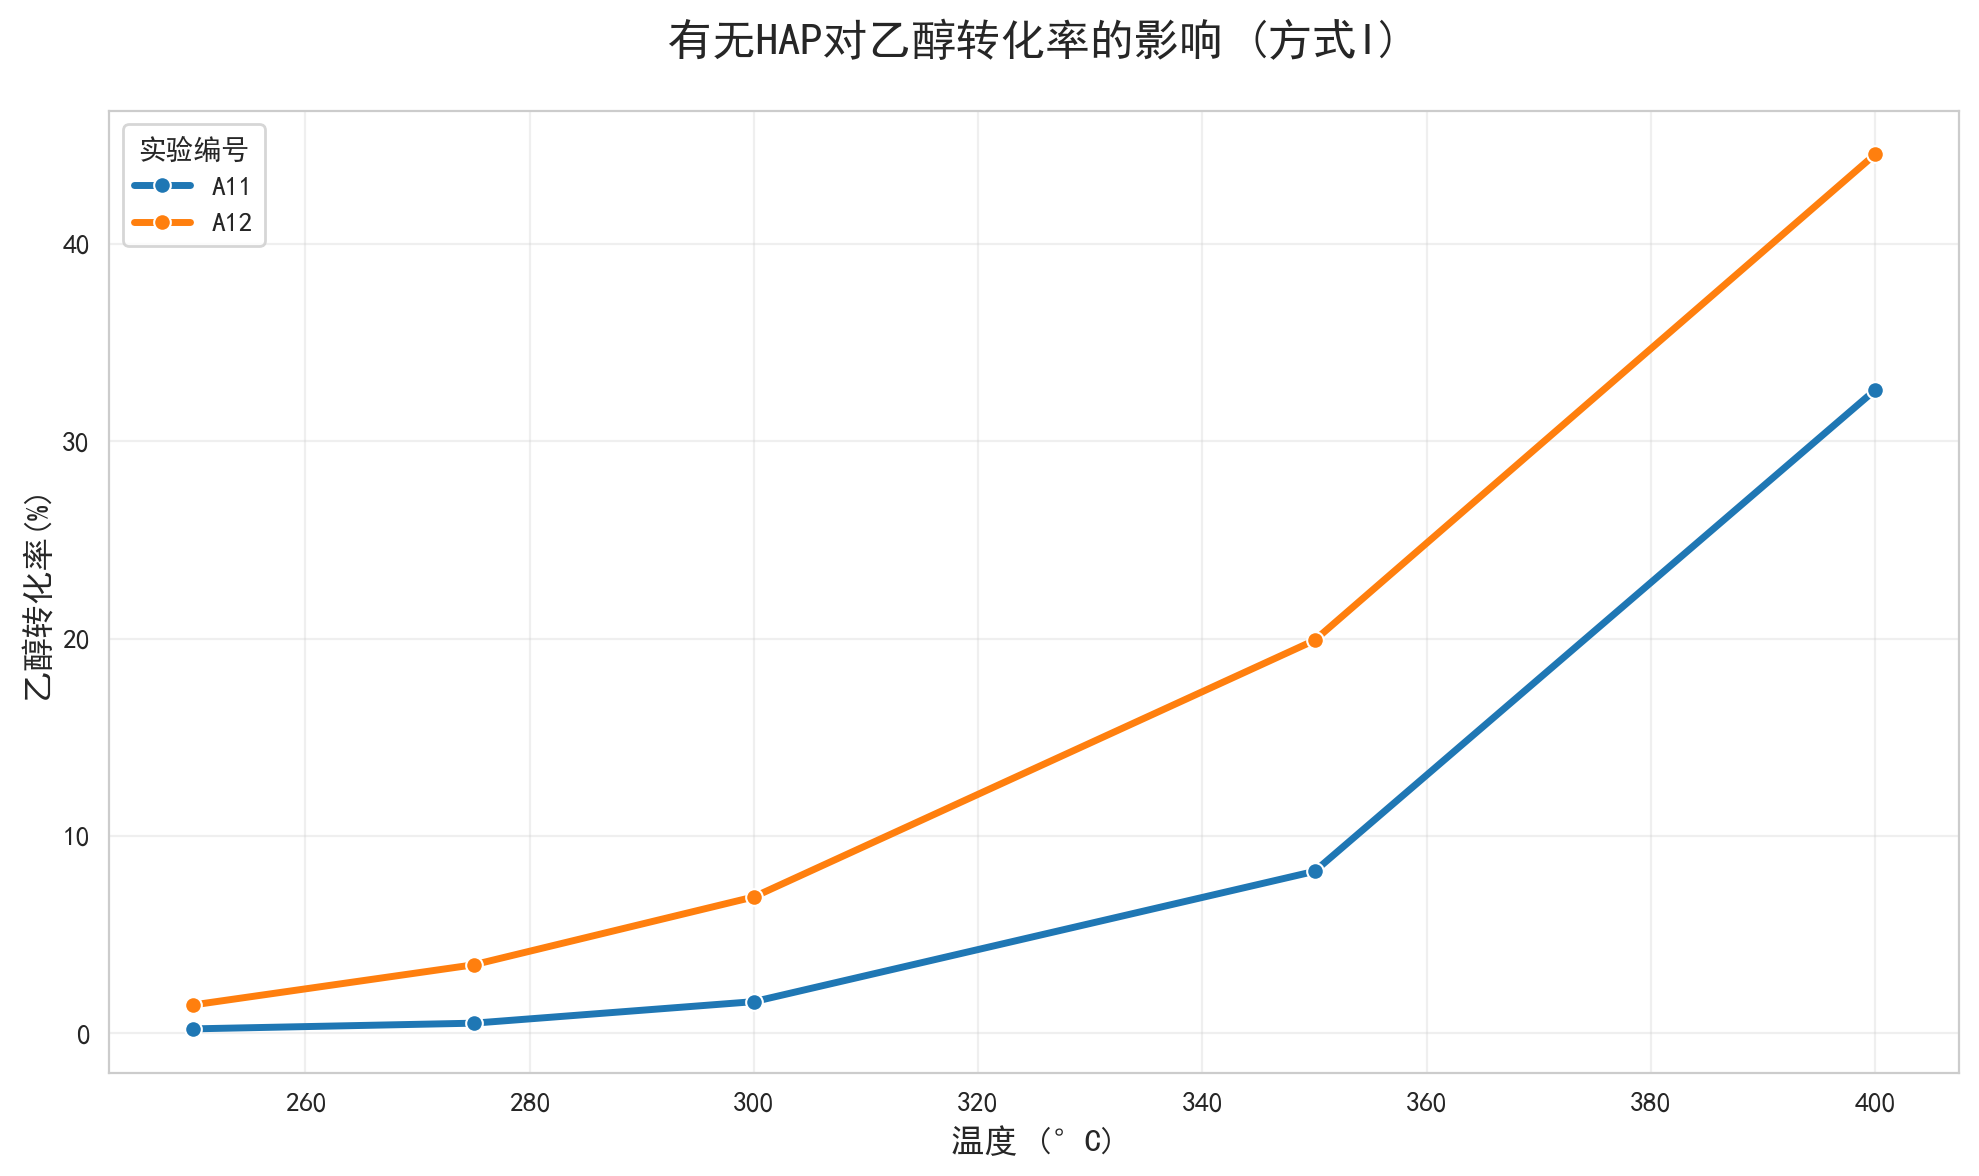
\includegraphics [scale=0.6]{图/2-4-1-2.png}
	\caption{有无HAP对乙醇转化率的影响 (方式I)} 
	\label{fig:1}
\end{figure}

结果显而易见,A11组中没有HAP,该组反应过程中的转化率和选择性都不及A12组。




\paragraph{总质量不变,Co与HAP质量比不同}
这个条件下仅有一组对照实验,绘制转化率和选择性图像如图18-19:

\begin{figure}[h]%[h]:固定作用
	\centering%置中
	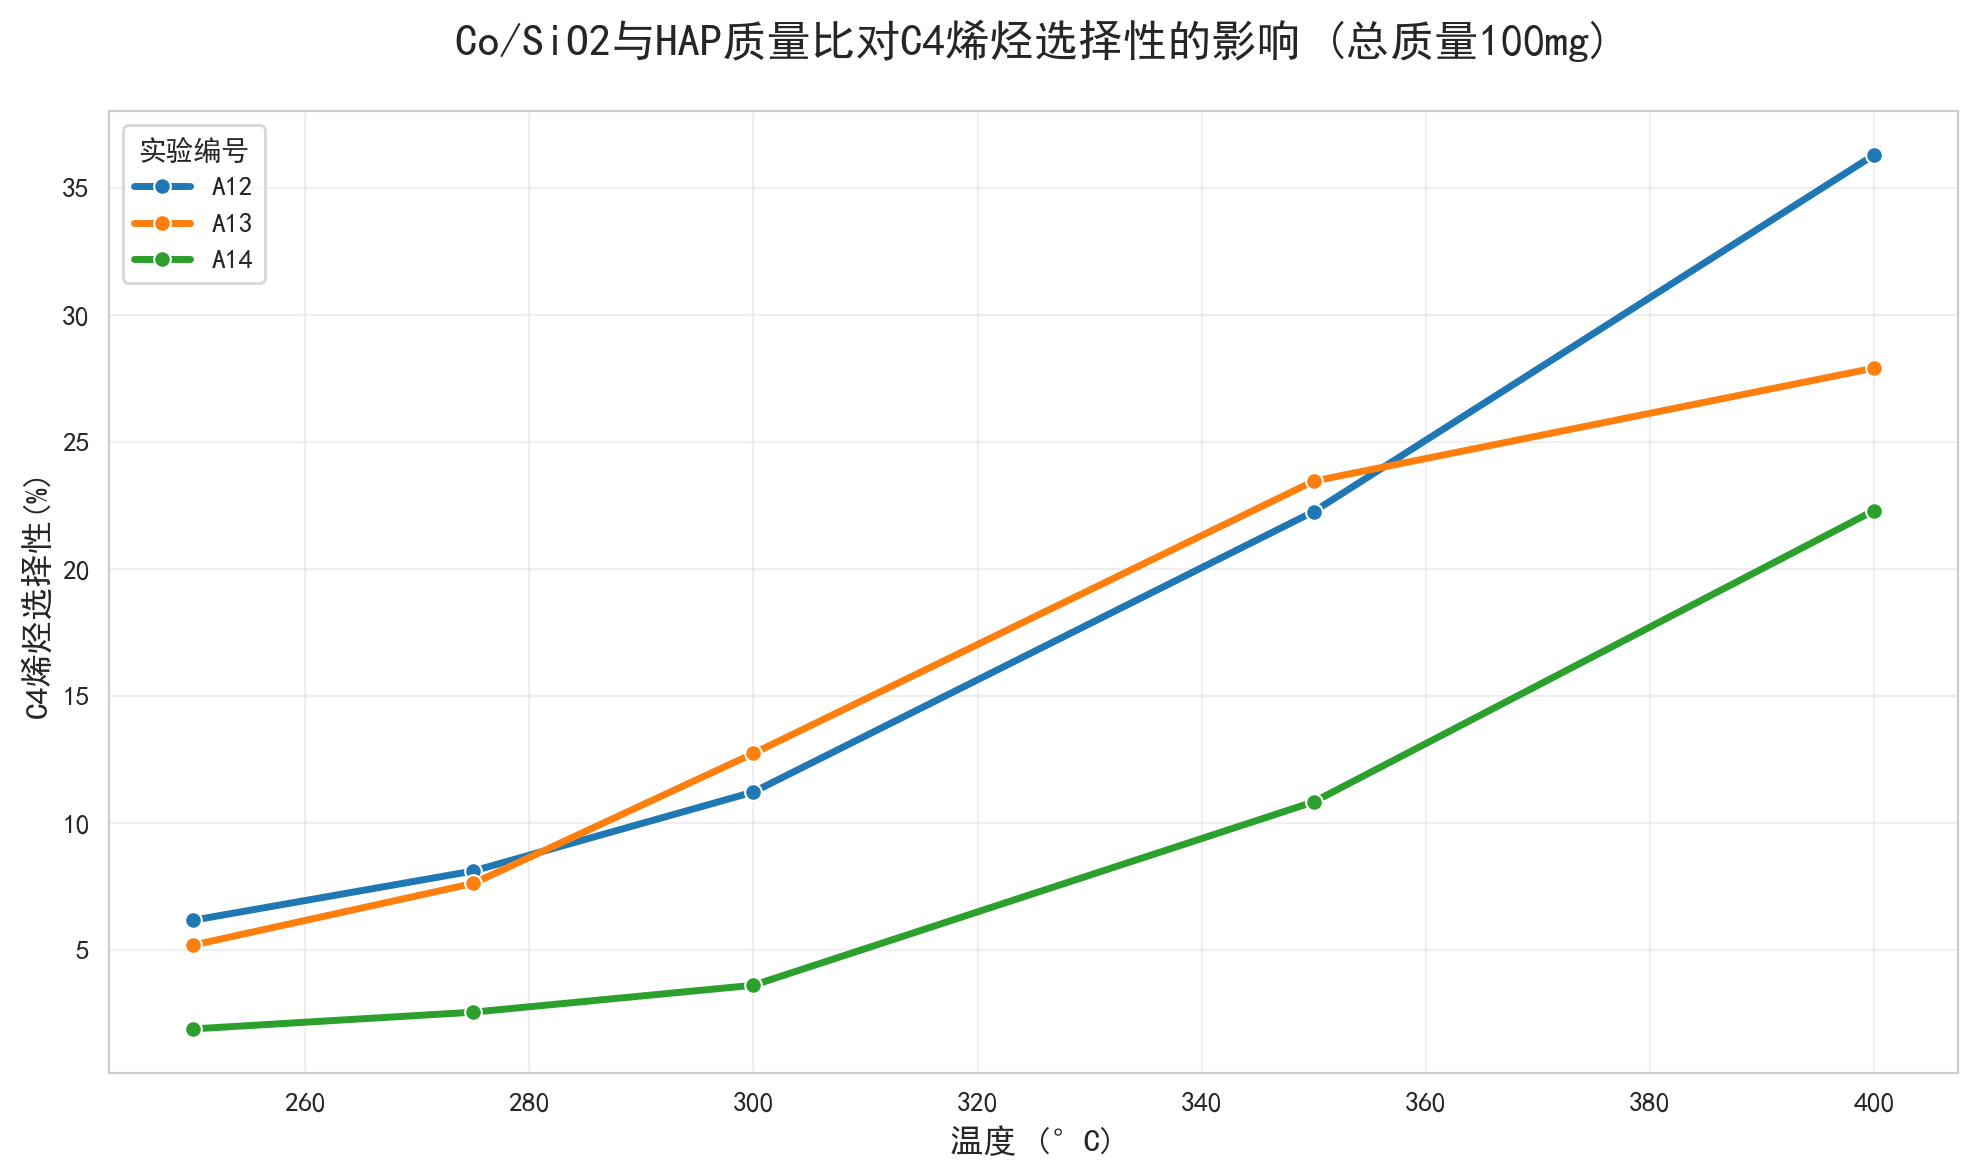
\includegraphics [scale=0.6]{图/2-5-1-1.png}
	\caption{Co/SiO2与HAP质量比对C4烯烃选择性的影响 (总质量100mg)} 
	\label{fig:1}
\end{figure}

\begin{figure}[h]%[h]:固定作用
	\centering%置中
	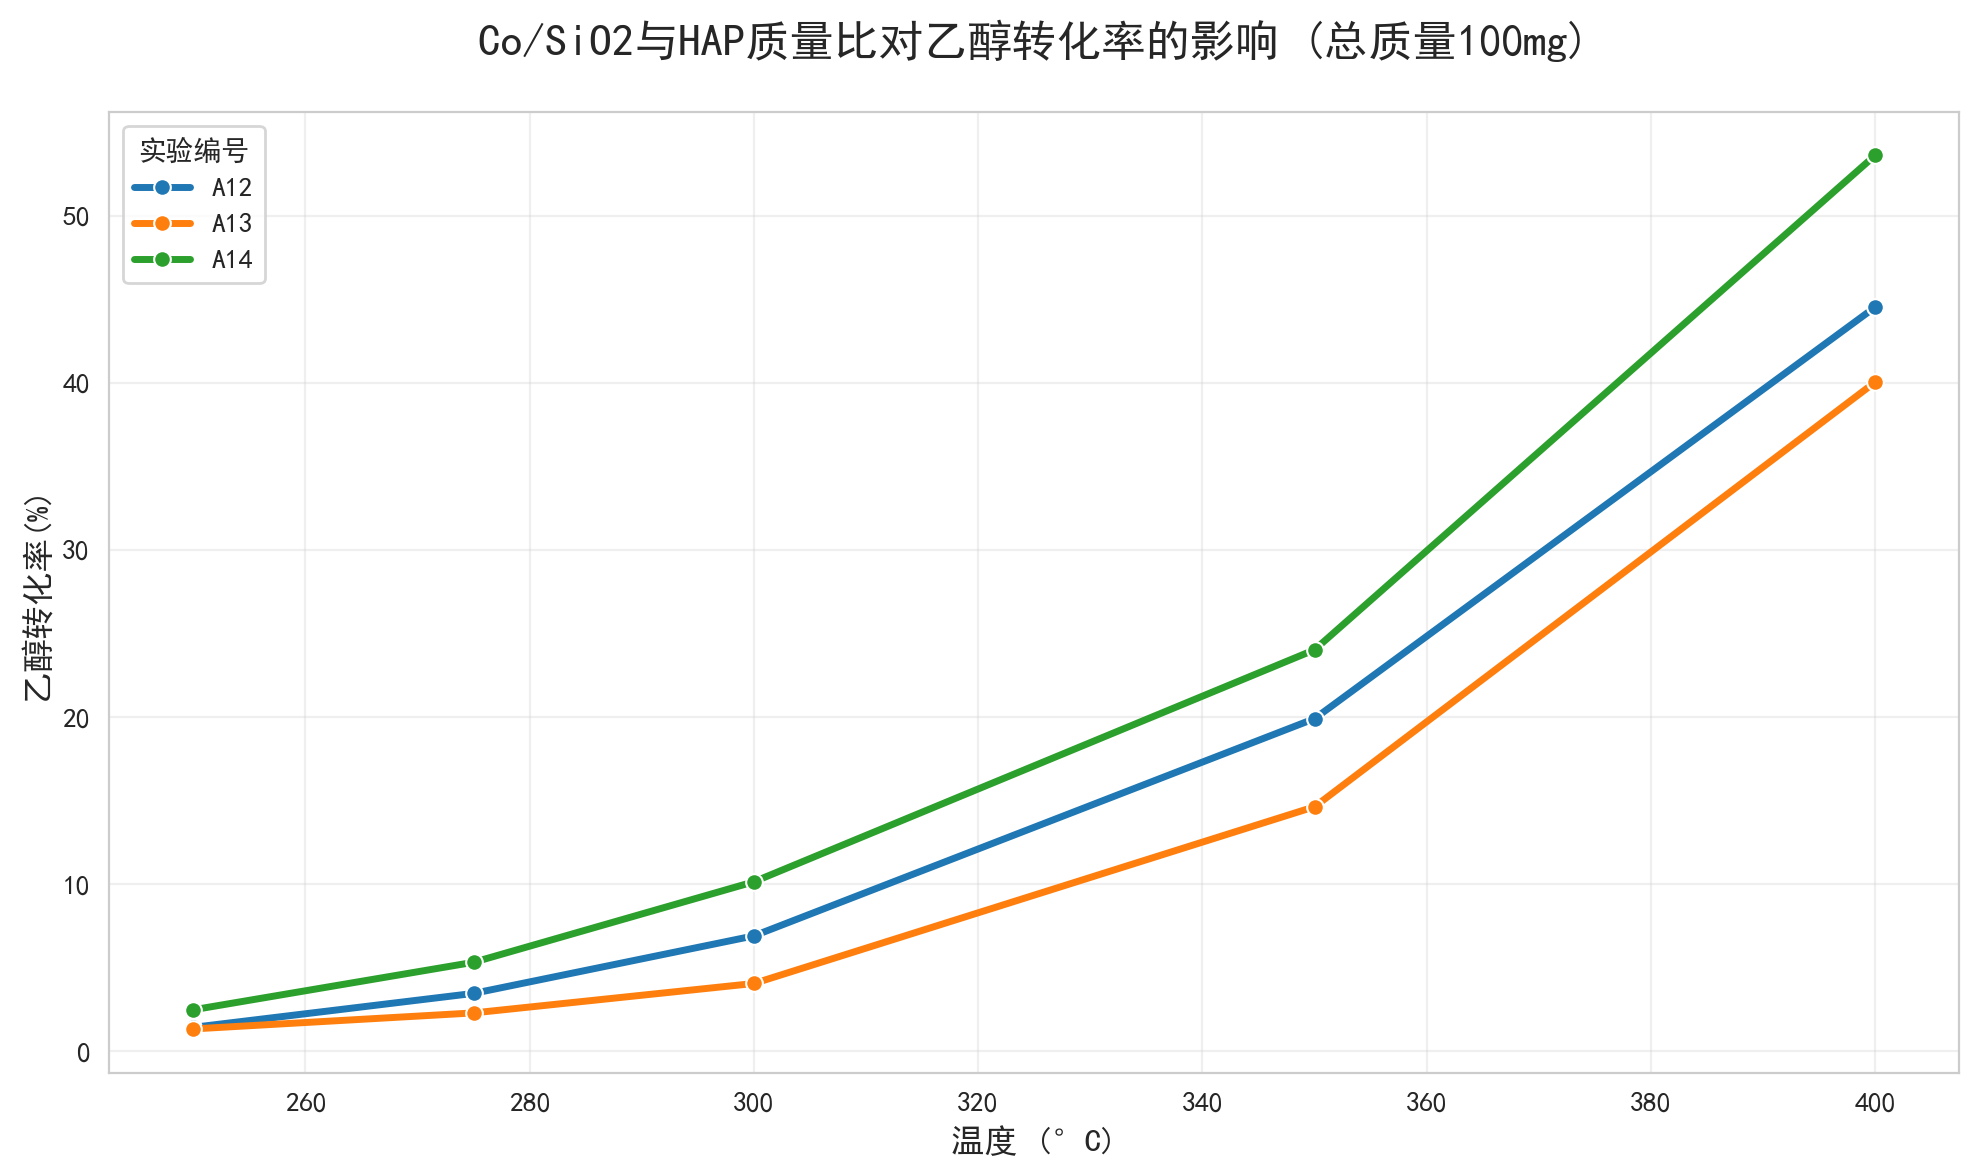
\includegraphics [scale=0.6]{图/2-5-1-2.png}
	\caption{Co/SiO2与HAP质量比对乙醇转化率的影响 (总质量100mg)} 
	\label{fig:1}
\end{figure}

大致情况下,质量不变,HAP的占比越高乙醇转化率越高,而对于 \( \text{C}_4 \) 烯烃选择性,在较低温度下,HAP占比较低情况下其变化一些影响不大,但在高温情况下选择性最高的还是比例1:1的催化剂组合,推测可能比例逐渐改变过程中,选择性结果先增大后降低,即在中间某个比例时达到最高选择性。


\paragraph{Co与HAP质量比1:1,总质量不同}
这一系列对照实验与上一系列对照实验思路大致相同,改变催化剂组合的总质量,针对B1、B2、B3、B4、B6组的对照实验,转化率和选择性图像如图20-21:

\begin{figure}[h]%[h]:固定作用
	\centering%置中
	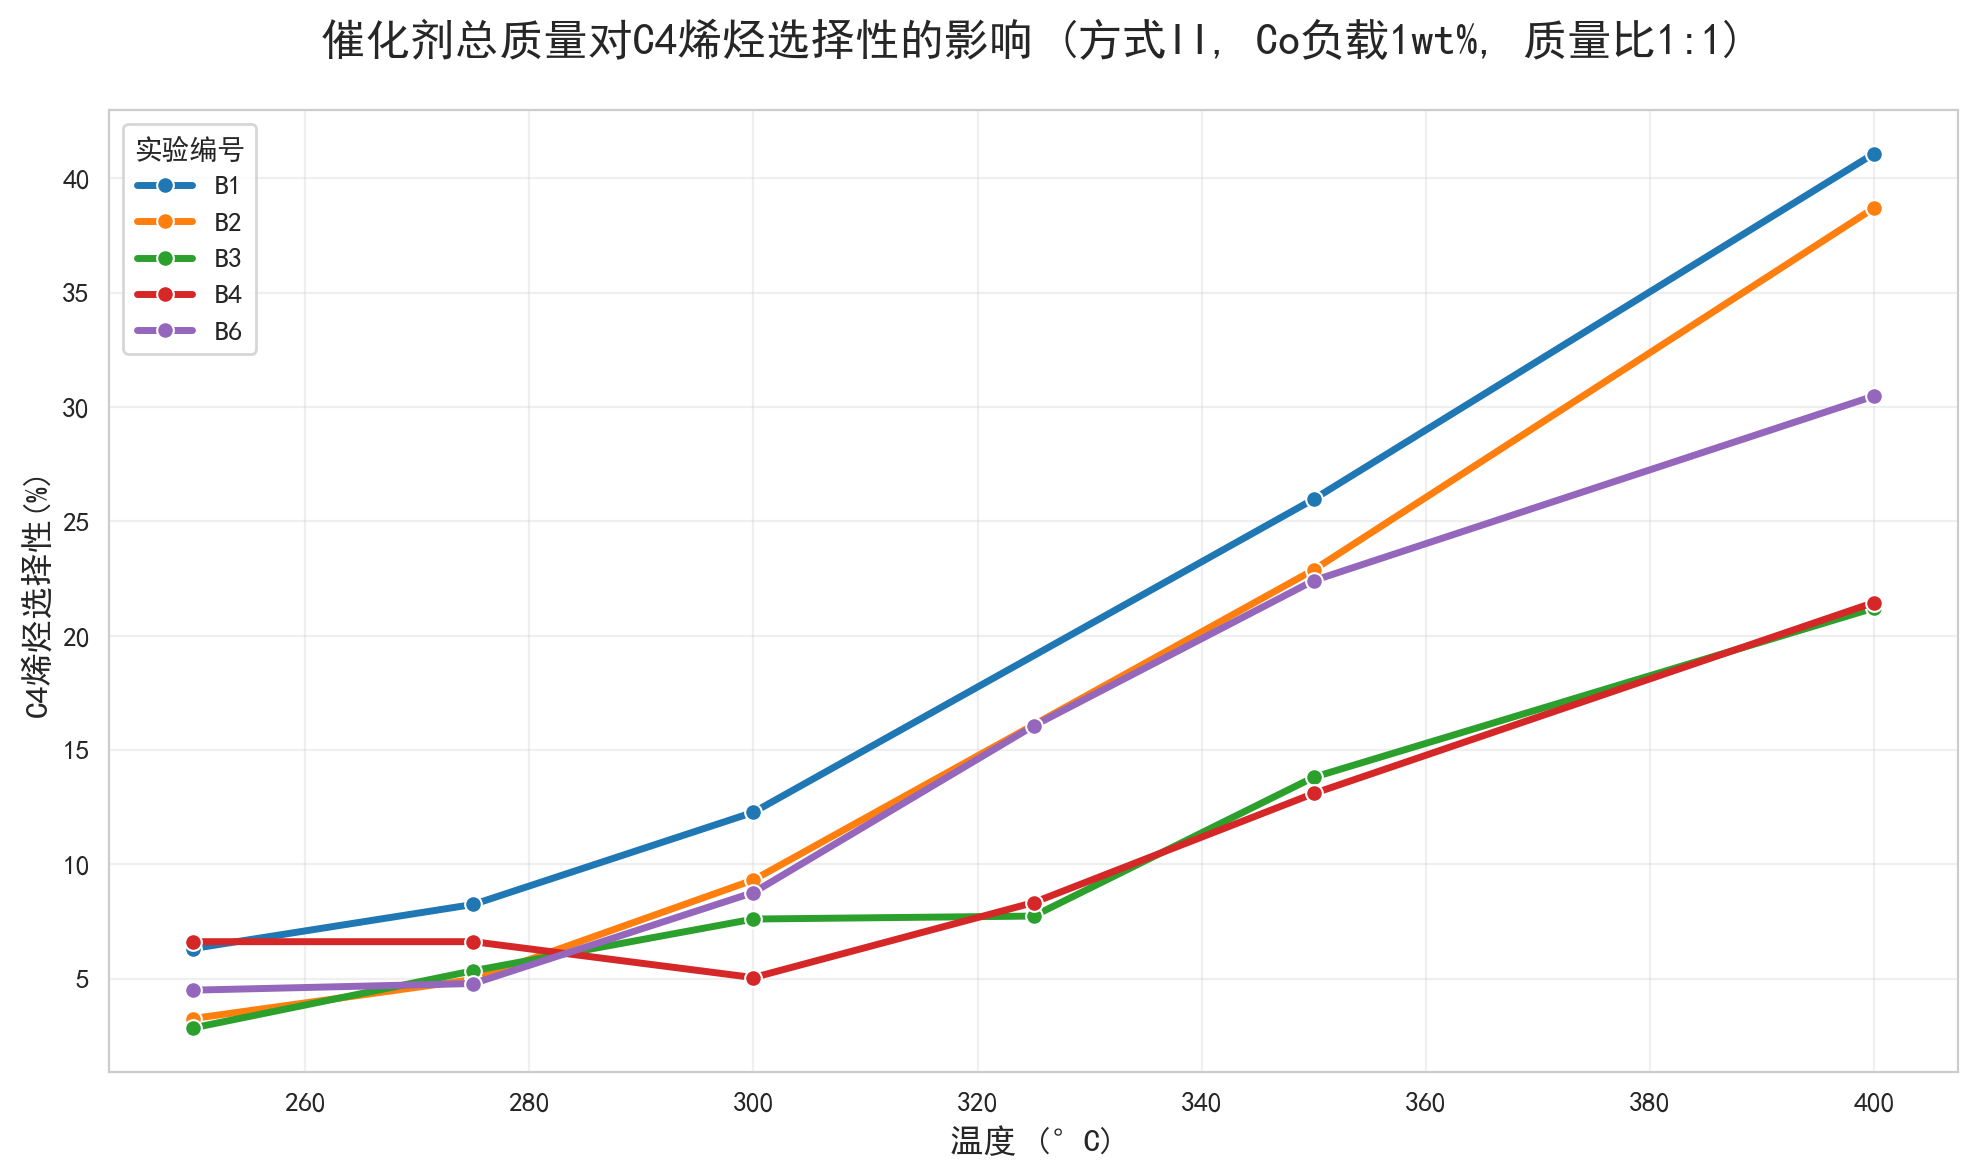
\includegraphics [scale=0.6]{图/2-6-1-1.png}
	\caption{催化剂总质量对C4烯烃选择性的影响 (方式II, Co负载1wt\%, 质量比1:1)} 
	\label{fig:1}
\end{figure}

\begin{figure}[h]%[h]:固定作用
	\centering%置中
	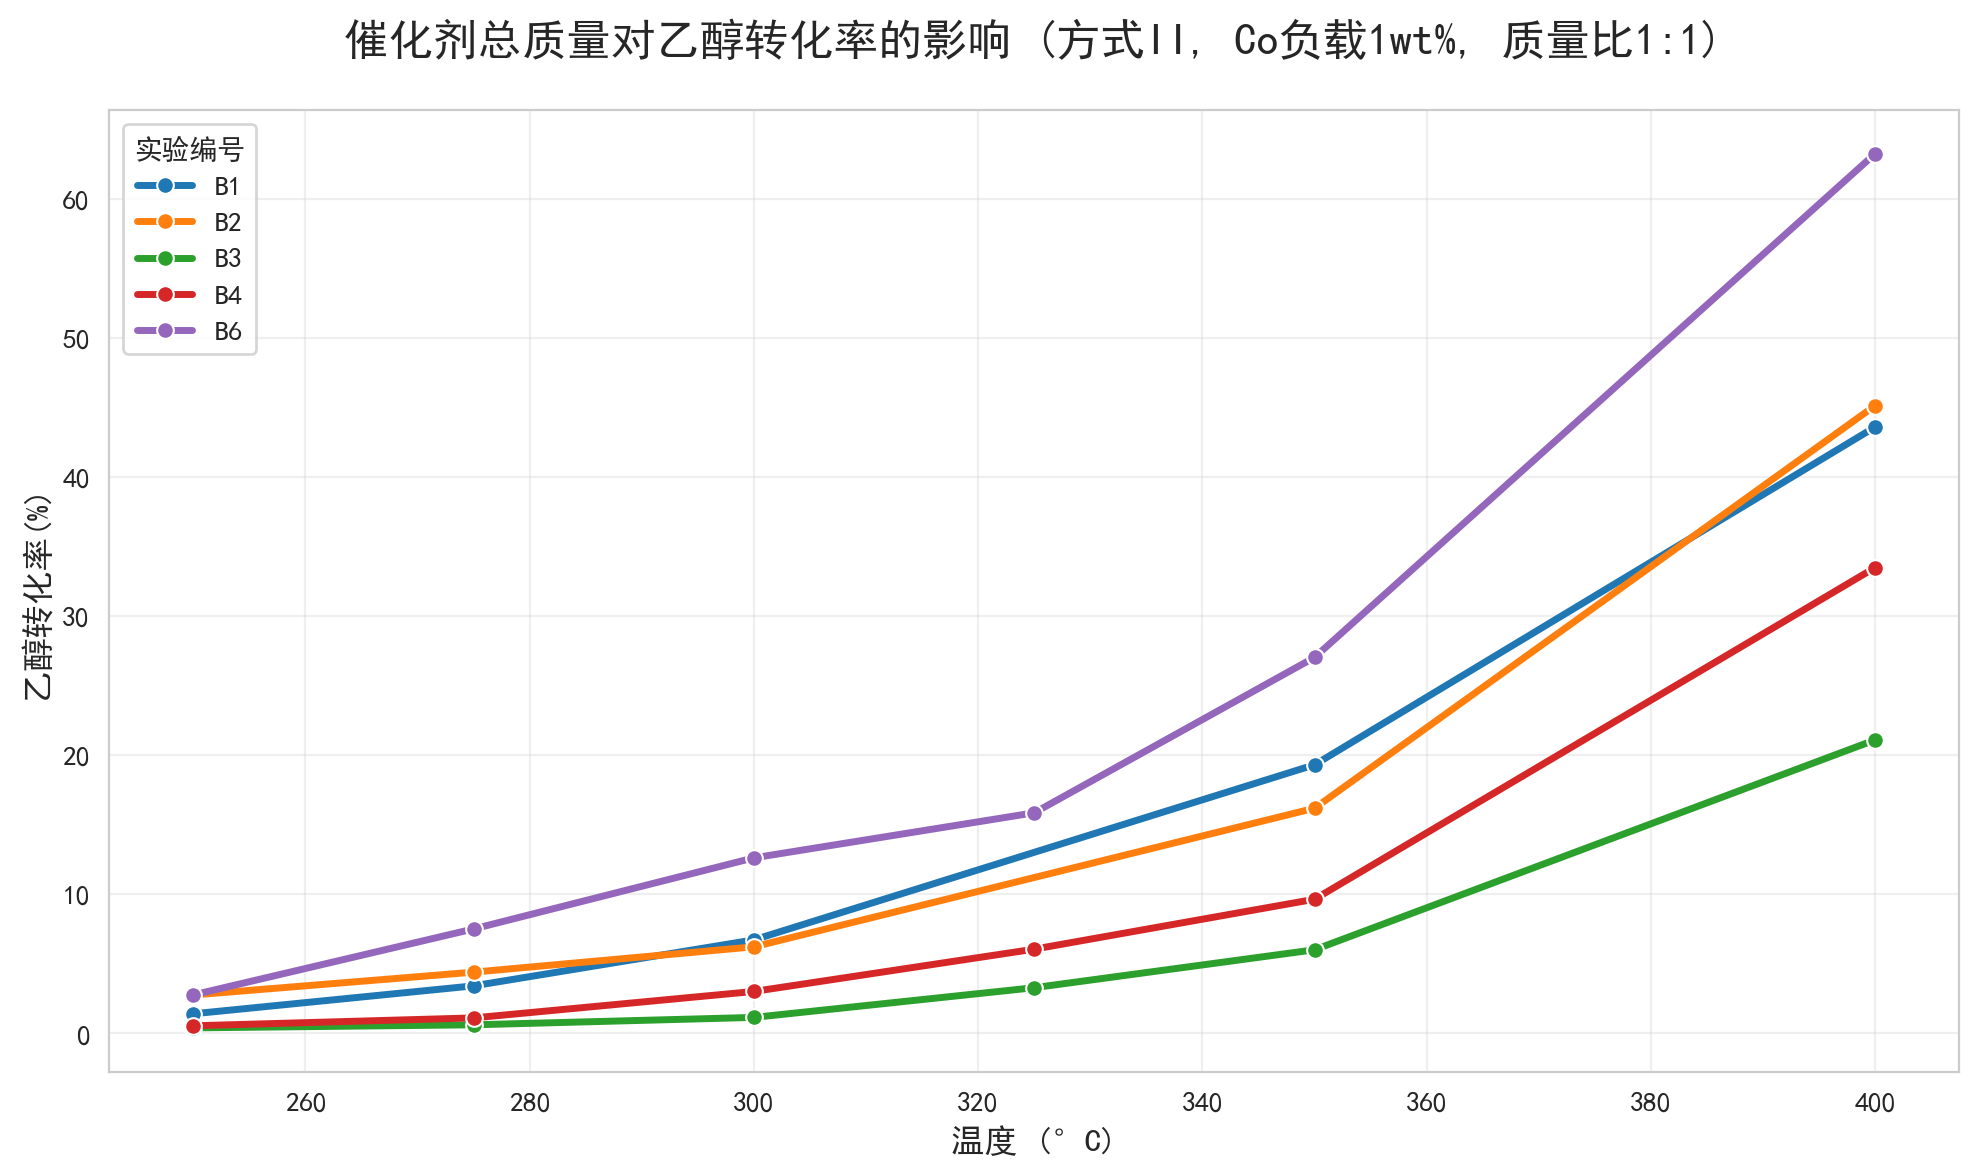
\includegraphics [scale=0.6]{图/2-6-1-2.png}
	\caption{催化剂总质量对乙醇转化率的影响 (方式II, Co负载1wt\%, 质量比1:1)} 
	\label{fig:1}
\end{figure}

大致对比下催化剂总质量越大越有利于转化率和选择性提高。


\subsubsection{回归拟合}	
以上只能算是表面分析,我们从各个组合内看到不同的变化,现在我们对不同催化剂组合内的变量进行回归拟合,从而在整体上了解他们之间的关系。首先分别提取所有催化剂组合的属性,提取属性过程中使用到正则化表达式,表达式相关代码如图22:

\begin{figure}[h]%[h]:固定作用
	\centering%置中
	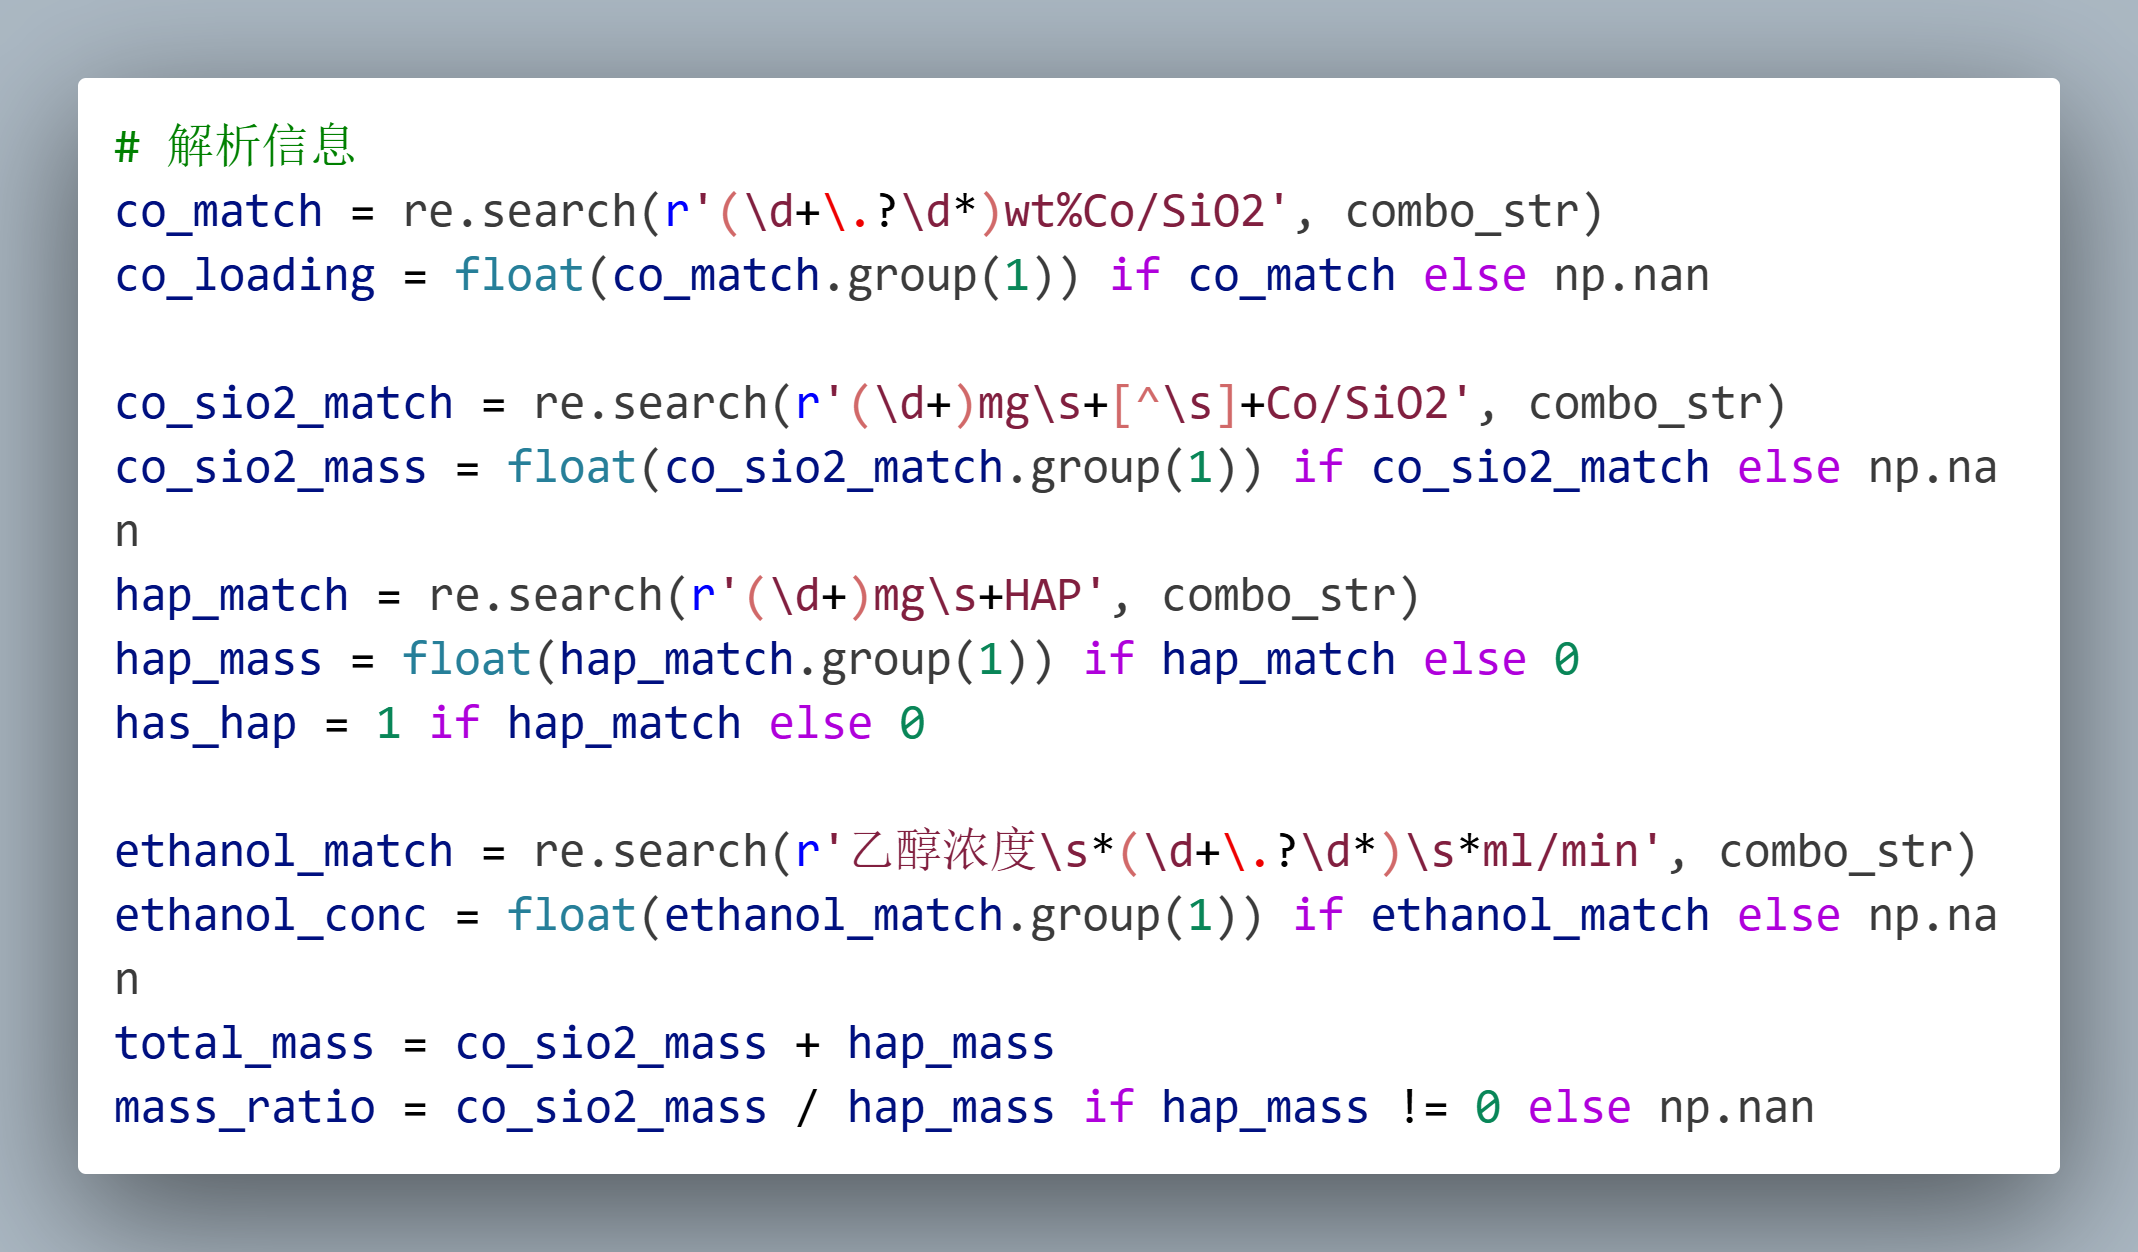
\includegraphics [scale=0.2]{图/code_1.png}
	\caption{Python正则化表达式代码} 
	\label{fig:1}
\end{figure}

现在我们得到了所有催化剂属性,根据每个组合中数据量少,可能导致过拟合,数据是高维数据,并且最后要具有较强可解释性的特点,我们选择岭回归。

岭回归是一种用于解决线性回归中多重共线性或过拟合问题的正则化方法。当自变量之间存在高度相关性,或特征数量较多时,普通最小二乘法估计的回归系数可能方差很大、不稳定。岭回归通过在损失函数中引入L2正则化项,对回归系数的平方和进行惩罚,从而缩小系数的绝对值,提高模型的稳定性和泛化能力。其目标是最小化以下损失函数:

$$
\text{Loss} = \sum_{i=1}^{n} (y_i - \mathbf{w}^T \mathbf{x}_i)^2 + \lambda \sum_{j=1}^{p} w_j^2
$$

其中,第一项是残差平方和,第二项是L2正则化项,$\lambda \geq 0$ 是正则化参数(也称惩罚系数),控制正则化的强度:$\lambda$ 越大,系数收缩越明显。岭回归的系数解具有闭式形式:

$$
\mathbf{w}_{\text{ridge}} = (\mathbf{X}^T \mathbf{X} + \lambda \mathbf{I})^{-1} \mathbf{X}^T \mathbf{y}
$$

其中 $\mathbf{X}$ 是特征矩阵,$\mathbf{y}$ 是目标向量,$\mathbf{I}$ 是单位矩阵。岭回归虽不能将系数压缩为零(不具特征选择功能),但能有效提升病态问题下的数值稳定性,广泛应用于高维数据建模。

现在我们选定特征有Co负载量(wt\%),Co/SiO2质量(mg)','HAP质量(mg)','乙醇浓度(ml/min)','温度',两个因变量乙醇转化率(\%)和 \( \text{C}_4 \) 烯烃选择性(\%)。由于各特征量纲不同,建模前对输入特征进行标准化处理(零均值、单位方差)。整个建模流程通过 Pipeline 实现标准化与回归的串联,确保数据预处理与模型训练的一致性。随后通过管道集成预处理与回归过程,正则化参数 $ \lambda $ 通过五折交叉验证结合网格搜索进行优化。搜索范围设置为 $ \lambda \in [10^{-3}, 10^{5}] $,共100个对数等间距候选值。模型选择依据为负均方误差,以最小化预测误差为目标。最后可得乙醇转化率岭回归路径图如图23:

\begin{figure}[h]%[h]:固定作用
	\centering%置中
	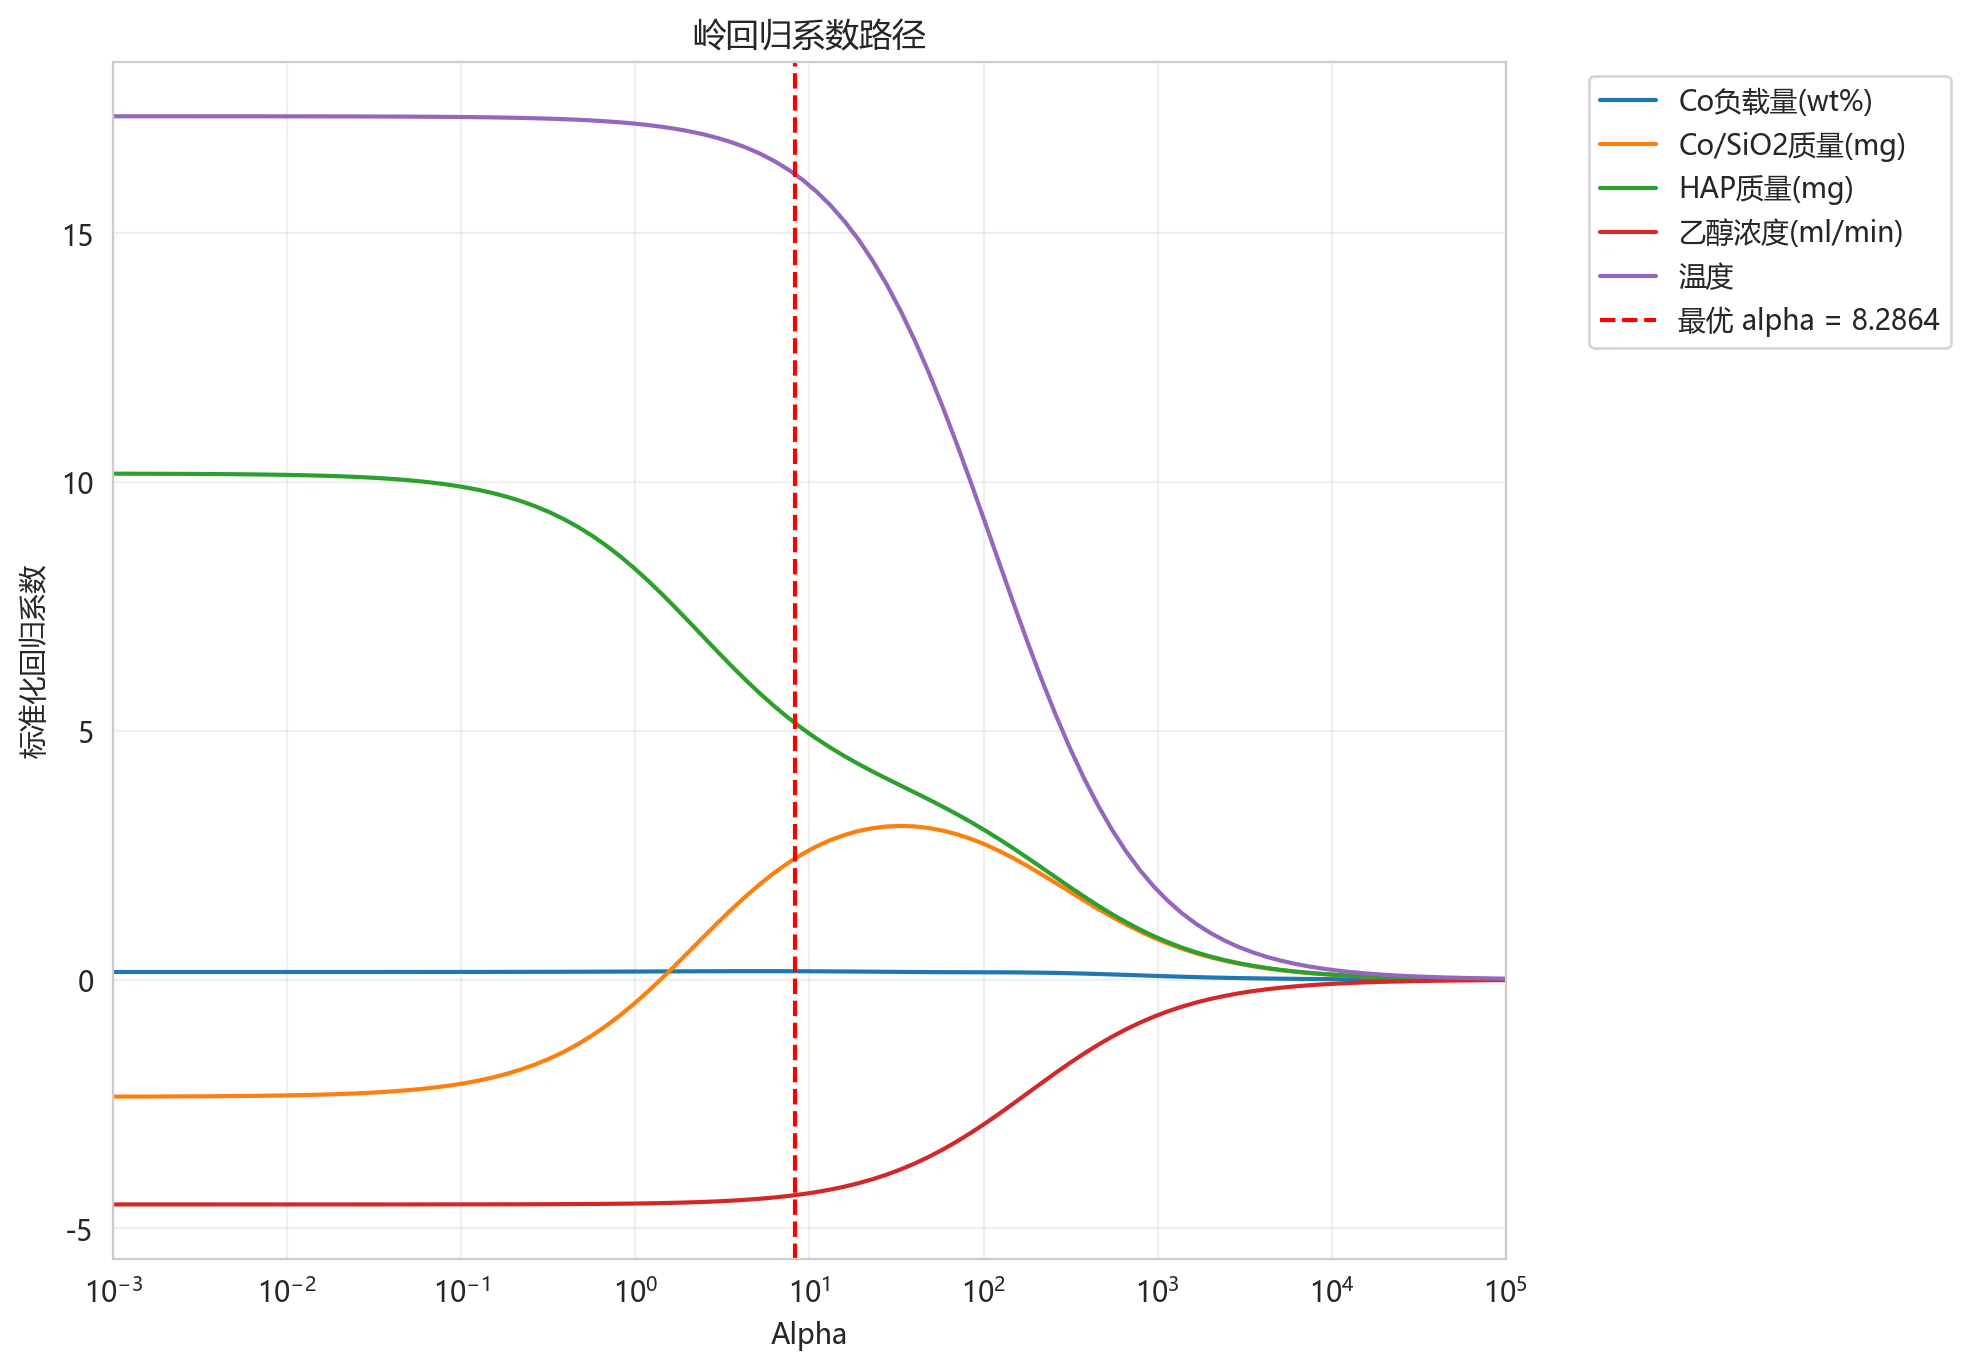
\includegraphics [scale=0.6]{图/ling-yichun.png}
	\caption{乙醇转化率岭回归系数路径} 
	\label{fig:1}
\end{figure}



最终得到最优 alpha = 8.2864,截距 = 21.9892,此时标准化回归系数如表2:

\newpage

\begin{table}[!htbp]
	\caption{乙醇转化率模型的标准化回归系数}
	\centering
	\begin{tabular}{l c}
		\hline
		\multicolumn{1}{c}{\textbf{特征名称}} & \textbf{标准化回归系数} \\
		\hline
		Co负载量(wt\%)      & 0.1697 \\
		Co/SiO2质量(mg)     & 2.4395 \\
		HAP质量(mg)         & 5.1538 \\
		乙醇浓度(ml/min)    & -4.3307 \\
		温度 (°C)                & 16.1869 \\
		\hline
		\label{tab:ridge_coefficients}
	\end{tabular}
\end{table}



同时可得 \( \text{C}_4 \) 烯烃选择性岭回归路径图如图24:
\begin{figure}[h]%[h]:固定作用
	\centering%置中
	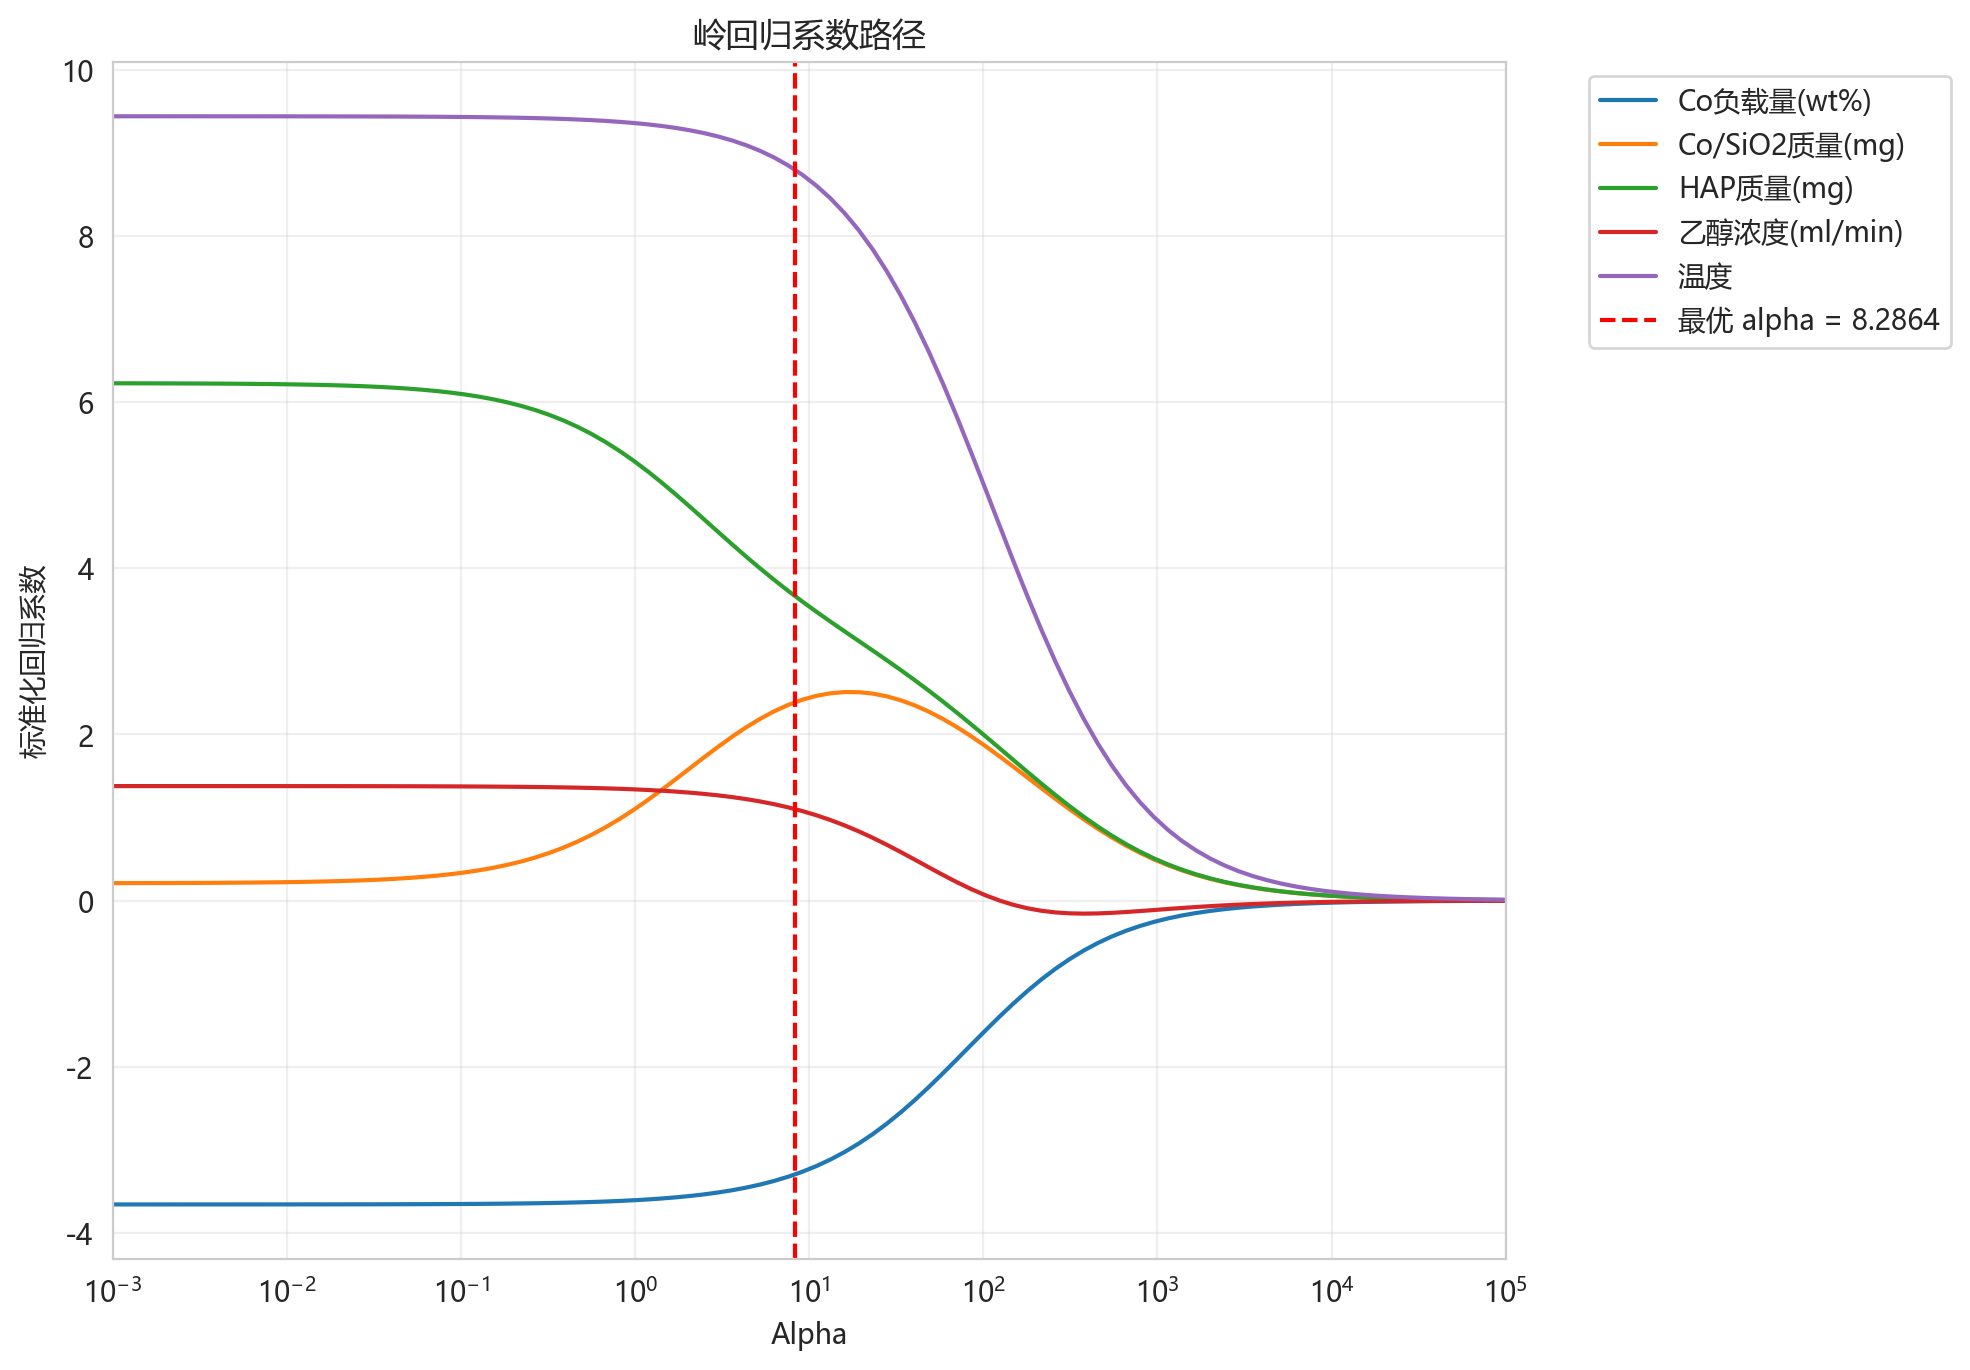
\includegraphics [scale=0.6]{图/ling-xuanzexing.png}
	\caption{ \( \text{C}_4 \) 烯烃选择性岭回归系数路径} 
	\label{fig:1}
\end{figure}

最终得到最优 alpha = 4.7149,截距 = 16.4508,此时标准化回归系数如表3:

\begin{table}[!htbp]
	\caption{C4烯烃选择性模型的标准化回归系数}
	\centering
	\begin{tabular}{l c}
		\hline
		\multicolumn{1}{c}{\textbf{特征名称}} & \textbf{标准化回归系数} \\
		\hline
		Co负载量(wt\%)      & -3.4383 \\
		Co/SiO2质量(mg)     & 2.1327 \\
		HAP质量(mg)         & 4.0744 \\
		乙醇浓度(ml/min)    & 1.2088 \\
		温度 (°C)               & 9.0609 \\
		\hline
		\label{tab:ridge_selectivity}
	\end{tabular}
\end{table}

\newpage


\subsubsection{结论}	
综合岭回归模型分析可知,温度和HAP质量是提升乙醇转化率与 \( \text{C}_4 \) 烯烃选择性的关键正向因素,二者均对两个目标具有显著促进作用,应优先优化。Co/SiO₂质量也有正向贡献,但影响相对较弱。值得注意的是,Co负载量虽对转化率略有提升,但显著抑制 \( \text{C}_4 \) 烯烃选择性,表明过高Co负载可能导致副反应加剧,不利于目标产物生成。此外,乙醇浓度的增加会降低转化率但提高选择性,反映出反应性能的权衡关系。因此,最优工艺条件应为:较高温度、适量HAP与Co/SiO₂用量、较低Co负载量,并在乙醇浓度上寻求转化率与选择性的平衡点。





\subsection{问题三的模型建立与求解}



\subsubsection{最优值提取}

在问题二数据基础上,进行加工,题目要求 \( \text{C}_4 \) 烯烃收率尽可能大,在名词解释中提到,其值为乙醇转化率*C4烯烃的选择性,简单想成病限制条件后,可在两种不同环境要求下选出所给数据中最优催化剂组合及温度。

在所有实验条件下, \( \text{C}_4 \) 烯烃收率最高为44.73\%,即全局最优解。此时催化剂详细信息为:A3 200mg 1wt\%Co/SiO2- 200mg HAP-乙醇浓度0.9ml/min,温度 400°C.

在温度低于350°C的条件下, \( \text{C}_4 \) 烯烃收率最高为17.26\%,即局部最优解。此时催化剂详细信息为:200mg 2wt\%Co/SiO2- 200mg HAP-乙醇浓度1.68ml/min,温度 325°C.


\subsubsection{深入分析与模型构建}
以上内容都仅存在于所给数据中,是离散的,不完整的,是片面性的,只在所得数据中是得不出更好的结果的,正如毛主席在《论持久战》中批评“速胜论”和“亡国论”两种错误观点时指出:“有些人只看到暂时的困难或局部的胜利,就悲观失望或盲目乐观,这是缺乏战略眼光的表现。”

我们选取Co负载量(wt\%), HAP质量分数, 乙醇浓度(ml/min), 温度四项作为自变量, \( \text{C}_4 \) 烯烃收率(\%)作为因变量构建多项式回归模型,采用二次多项式,因为经过测试,高次会造成过拟合。最终可得多项式回归模型R²得分: 0.8619.根据所得多项式回归,使用网格搜索,定义搜索范围,分别在全局和限制温度低于350°C时的最优解。最终得到如下结果:

在所有实验条件下, \( \text{C}_4 \) 烯烃收率预测最高为52.03\%,即局部最优解。此时催化剂详细预测信息为:120mg 5wt\%Co/SiO2- 80mg HAP-乙醇浓度0.30ml/min,温度 450°C.

在温度低于350°C的条件下, \( \text{C}_4 \) 烯烃收率预测最高为21.70\%,即局部最优解。此时催化剂详细预测信息为:180mg 5wt\%Co/SiO2- 20mg HAP-乙醇浓度0.30ml/min,温度 350°C.



\subsection{问题四}

若允许再增加五次实验,应基于前三问的建模分析结果,科学设计实验方案,以最大化信息获取效率,进一步逼近最优工艺条件。当前已有数据分析表明,温度、HAP质量、Co/SiO₂质量、Co负载量及乙醇浓度均对乙醇转化率和C₄烯烃选择性具有不同程度的影响,且通过多项式回归模型预测出理论上的 \( \text{C}_4 \) 烯烃收率最优值可能高于现有实验数据所能达到的水平。因此,新增实验应聚焦于探索当前数据覆盖不足或模型预测性能提升潜力较大的参数区域。

首先,根据问题三中多项式回归模型的预测结果,在全局范围内C₄烯烃收率的理论最大值出现在温度450°C、Co负载量5wt\%、Co/SiO₂质量120mg、HAP质量80mg、乙醇浓度0.30ml/min的条件下。然而该组合尚未在实际实验中验证,且高温条件下催化剂稳定性可能存在挑战,因此建议安排一次实验验证该高收率预测点的实际可行性,实验条件设定为:装料方式I(延续A组体系便于比较),120mg 5wt\%Co/SiO₂-80mg HAP,乙醇浓度0.30ml/min,温度450°C,反应时间控制在60分钟以内以初步评估活性保持能力。

其次,考虑工业应用中对能耗与安全性的要求,低温高效工艺更具现实意义。问题三预测在温度≤350°C时,最优收率对应条件为180mg 5wt\%Co/SiO₂-20mg HAP,乙醇浓度0.30ml/min,温度350°C。此条件下HAP占比极低,是否仍能维持良好的催化协同效应尚不明确。为此,设计第二次实验对该预测点进行验证,采用相同装料方式I,严格控制变量,观察其在350°C下的实际收率表现及产物分布稳定性。

第三,从控制变量分析中发现,Co负载量对C₄烯烃选择性有显著负向影响(岭回归系数为-3.4383),而现有实验中Co负载量最高仅为5wt\%,未涵盖更高范围。为探究Co负载量的极限影响及是否存在选择性拐点,设计第三次实验:固定其他条件(如A3组基础配置:200mg Co/SiO₂-200mg HAP,乙醇浓度0.9ml/min,温度400°C),将Co负载量提升至8wt\%,考察高Co浓度下主副反应竞争关系的变化趋势。

第四,附件2的稳定性测试显示,催化剂在长时间运行后乙醇转化率持续下降,表明存在失活现象。为探索催化剂寿命与结构稳定性的关联,设计第四次实验:选取当前收率较高的A3组合(200mg 1wt\%Co/SiO₂-200mg HAP,0.9ml/min,400°C),延长反应时间至400分钟,每隔60分钟记录一次性能数据,重点监测乙醇转化率、C₄烯烃选择性及积碳前驱体(如乙醛、芳香族化合物)的生成趋势,为后续催化剂抗积碳改性提供依据。

第五,考虑到装料方式II(B组)在部分条件下表现出不同的响应特性,但整体实验点较少,难以构建稳健模型。为增强模型泛化能力,设计第五次实验:在装料方式II下复现一组高收率条件,如B1的扩展实验——保持Co负载1wt\%、质量比1:1、总质量100mg,调整温度至400°C,乙醇浓度1.68ml/min,以检验不同装料方式下最优路径的一致性与差异性。

综上所述,新增五次实验分别围绕“高收率预测验证”、“低温优化验证”、“关键参数拓展”、“稳定性深化研究”和“装料方式对比”五个维度展开,既覆盖了模型预测的极端优值点,也补充了现有数据在参数空间中的空白区域,同时兼顾了实际应用中的稳定性需求。该设计遵循“由面到点、由稳到优”的实验优化逻辑,能够在有限资源下最大程度提升对系统行为的理解深度,为最终确定最优催化剂组合与工艺条件提供坚实的数据支撑。 %插入模型的建立与求解   MakeModel.tex

\section{模型的评价}

\subsection{模型的优点}%(建模方法创新、求解特色等) 

\begin{itemize}
	%得到满意的解
	%较好地解决了…问题
	%使模型得到简化 
	%使结果更合理,避免…带来的较大误差
	%使问题描述比较清晰
	%减少大的计算量
	
	\item[(1)] 模型体系具有较强的系统性与层次性。针对不同问题采用由浅入深的分析思路,问题一通过数据可视化与相关性分析实现对变量关系的直观把握,问题二结合控制变量法与岭回归建模,在保留物理意义的同时提升了量化分析能力,问题三进一步引入多项式回归与网格搜索,实现了从离散数据向连续参数空间的拓展,整体建模过程逻辑清晰、层层递进,符合科学研究的认知规律。
	
	\item[(2)] 所选方法兼顾可解释性与预测能力。在问题二中采用岭回归处理高维特征数据,有效缓解了多重共线性带来的模型不稳定问题,且标准化回归系数便于直接比较各因素的影响方向与强度,为工艺优化提供了明确的指导依据;在问题三中构建二次多项式回归模型,既能捕捉关键变量间的非线性关系,又避免了高阶项导致的过拟合现象,模型R²达到0.8619,具备良好的拟合优度与外推潜力。
	
	\item[(3)] 实验设计与模型驱动紧密结合。问题四的新增实验方案并非凭空设想,而是基于前三问的建模结果进行反向推演,聚焦于高收率预测点验证、关键参数边界探索、稳定性深化研究等核心方向,体现了“以模型引导实验、以实验反馈模型”的闭环优化思想,提高了后续实验的信息获取效率和工程应用价值。
	
\end{itemize}	

\subsection{模型的缺点}
%主观性过强
%建立在什么的前提条件下
%有一定的局限性
%存在不确定性
%有一定的偏差

\begin{itemize}
	
	\item[(1)] 数据局限性对模型泛化能力构成制约。附件一所提供的催化剂组合数量有限,且部分变量水平设置不均衡(如Co负载量未超过5wt\%,温度区间跳跃较大),导致模型训练所依赖的样本覆盖范围不足,尤其在进行网格搜索预测时,可能存在超出实际可行域的风险,影响最优条件的实际可操作性。
	
	\item[(2)] 多项式回归模型虽避免了过拟合,但仍存在理论假设限制。二次多项式形式虽能描述一定的非线性趋势,但难以刻画复杂催化反应中可能出现的阈值效应或突变行为(如催化剂相变、积碳临界点等),且模型未考虑变量间的交互作用项精细化建模,可能弱化某些协同效应的表达能力。
	
	\item[(3)] 稳定性因素尚未完全纳入建模框架。尽管附件二揭示了催化剂随时间推移存在活性衰减现象,但在前三问的模型构建中主要关注稳态性能指标(转化率、选择性、收率),未将时间维度或失活动力学纳入回归模型,导致最优条件的选取更多反映瞬时性能而非长期运行下的综合效益,可能影响工业应用中的实际可行性。
	
\end{itemize}	
\subsection{模型的推广}
%对本文中的模型给出比较客观的评价,必须实事求是,有根据,以便评卷人参考。
%推广和优化,需要花费功夫想出合理的、甚至可以合理改变题目给出的条件的、不一定可行但是具有一定想象空间的准理想的方法、模型。由此做出一些改进方向,也可以是参赛者一些来不及实现的思路。


\begin{itemize}
	
	\item[(1)] 本研究建立的“可视化—控制变量—回归建模—预测优化”四步分析流程,可推广至其他多因素催化反应系统的工艺优化中,尤其适用于实验数据量中等、变量维度较高的场景,具有较强的通用性和移植性。
	
	\item[(2)] 岭回归与多项式回归相结合的建模范式,可用于处理类似存在多重共线性且需探索非线性关系的工程建模问题,如材料配比设计、燃烧效率优化、电池性能预测等领域,具备一定的方法论参考价值。
	
	\item[(3)] 基于模型预测指导新增实验的设计思路,可为实验室阶段的小样本优化提供科学路径,实现“数据驱动+机理认知”的融合式研发,有助于缩短工艺开发周期,降低试错成本,适用于资源受限条件下的高效科研决策支持。
	
\end{itemize}	 %插入模型评价	ModelEvaluation.tex

\newpage
%附录
\appendix
%附录需重新起页,论文附录至少应包括参赛论文的所有源程序代码,如实际使用的软件名称、命令和编写的全部可运行的源程序(含EXCEL、SPSS等软件的交互命令);通常还应包括自主查阅使用的数据等资料。赛题中提供的数据不要放在附录。如果缺少必要的源程序或程序不能运行(或者运行结果与正文不符),可能会被取消评奖资格。如果确实没有源程序,也应在论文附录中明确说明“本论文没有源程序”。 	

\section{代码程序}
% 插入Python代码
\lstinputlisting[style=Python, caption={问题一所需Python代码}]{code/code_1.py}

\lstinputlisting[style=Python, caption={问题二所需Python代码}]{code/code_2.py}

\lstinputlisting[style=Python, caption={问题三所需Python代码}]{code/code_3.py}


\section{详细图表}

\setcounter{figure}{0}
\setcounter{table}{0}

\subsection*{问题一详细数据表}

\begin{figure}[h]%[h]:固定作用
	\centering%置中
	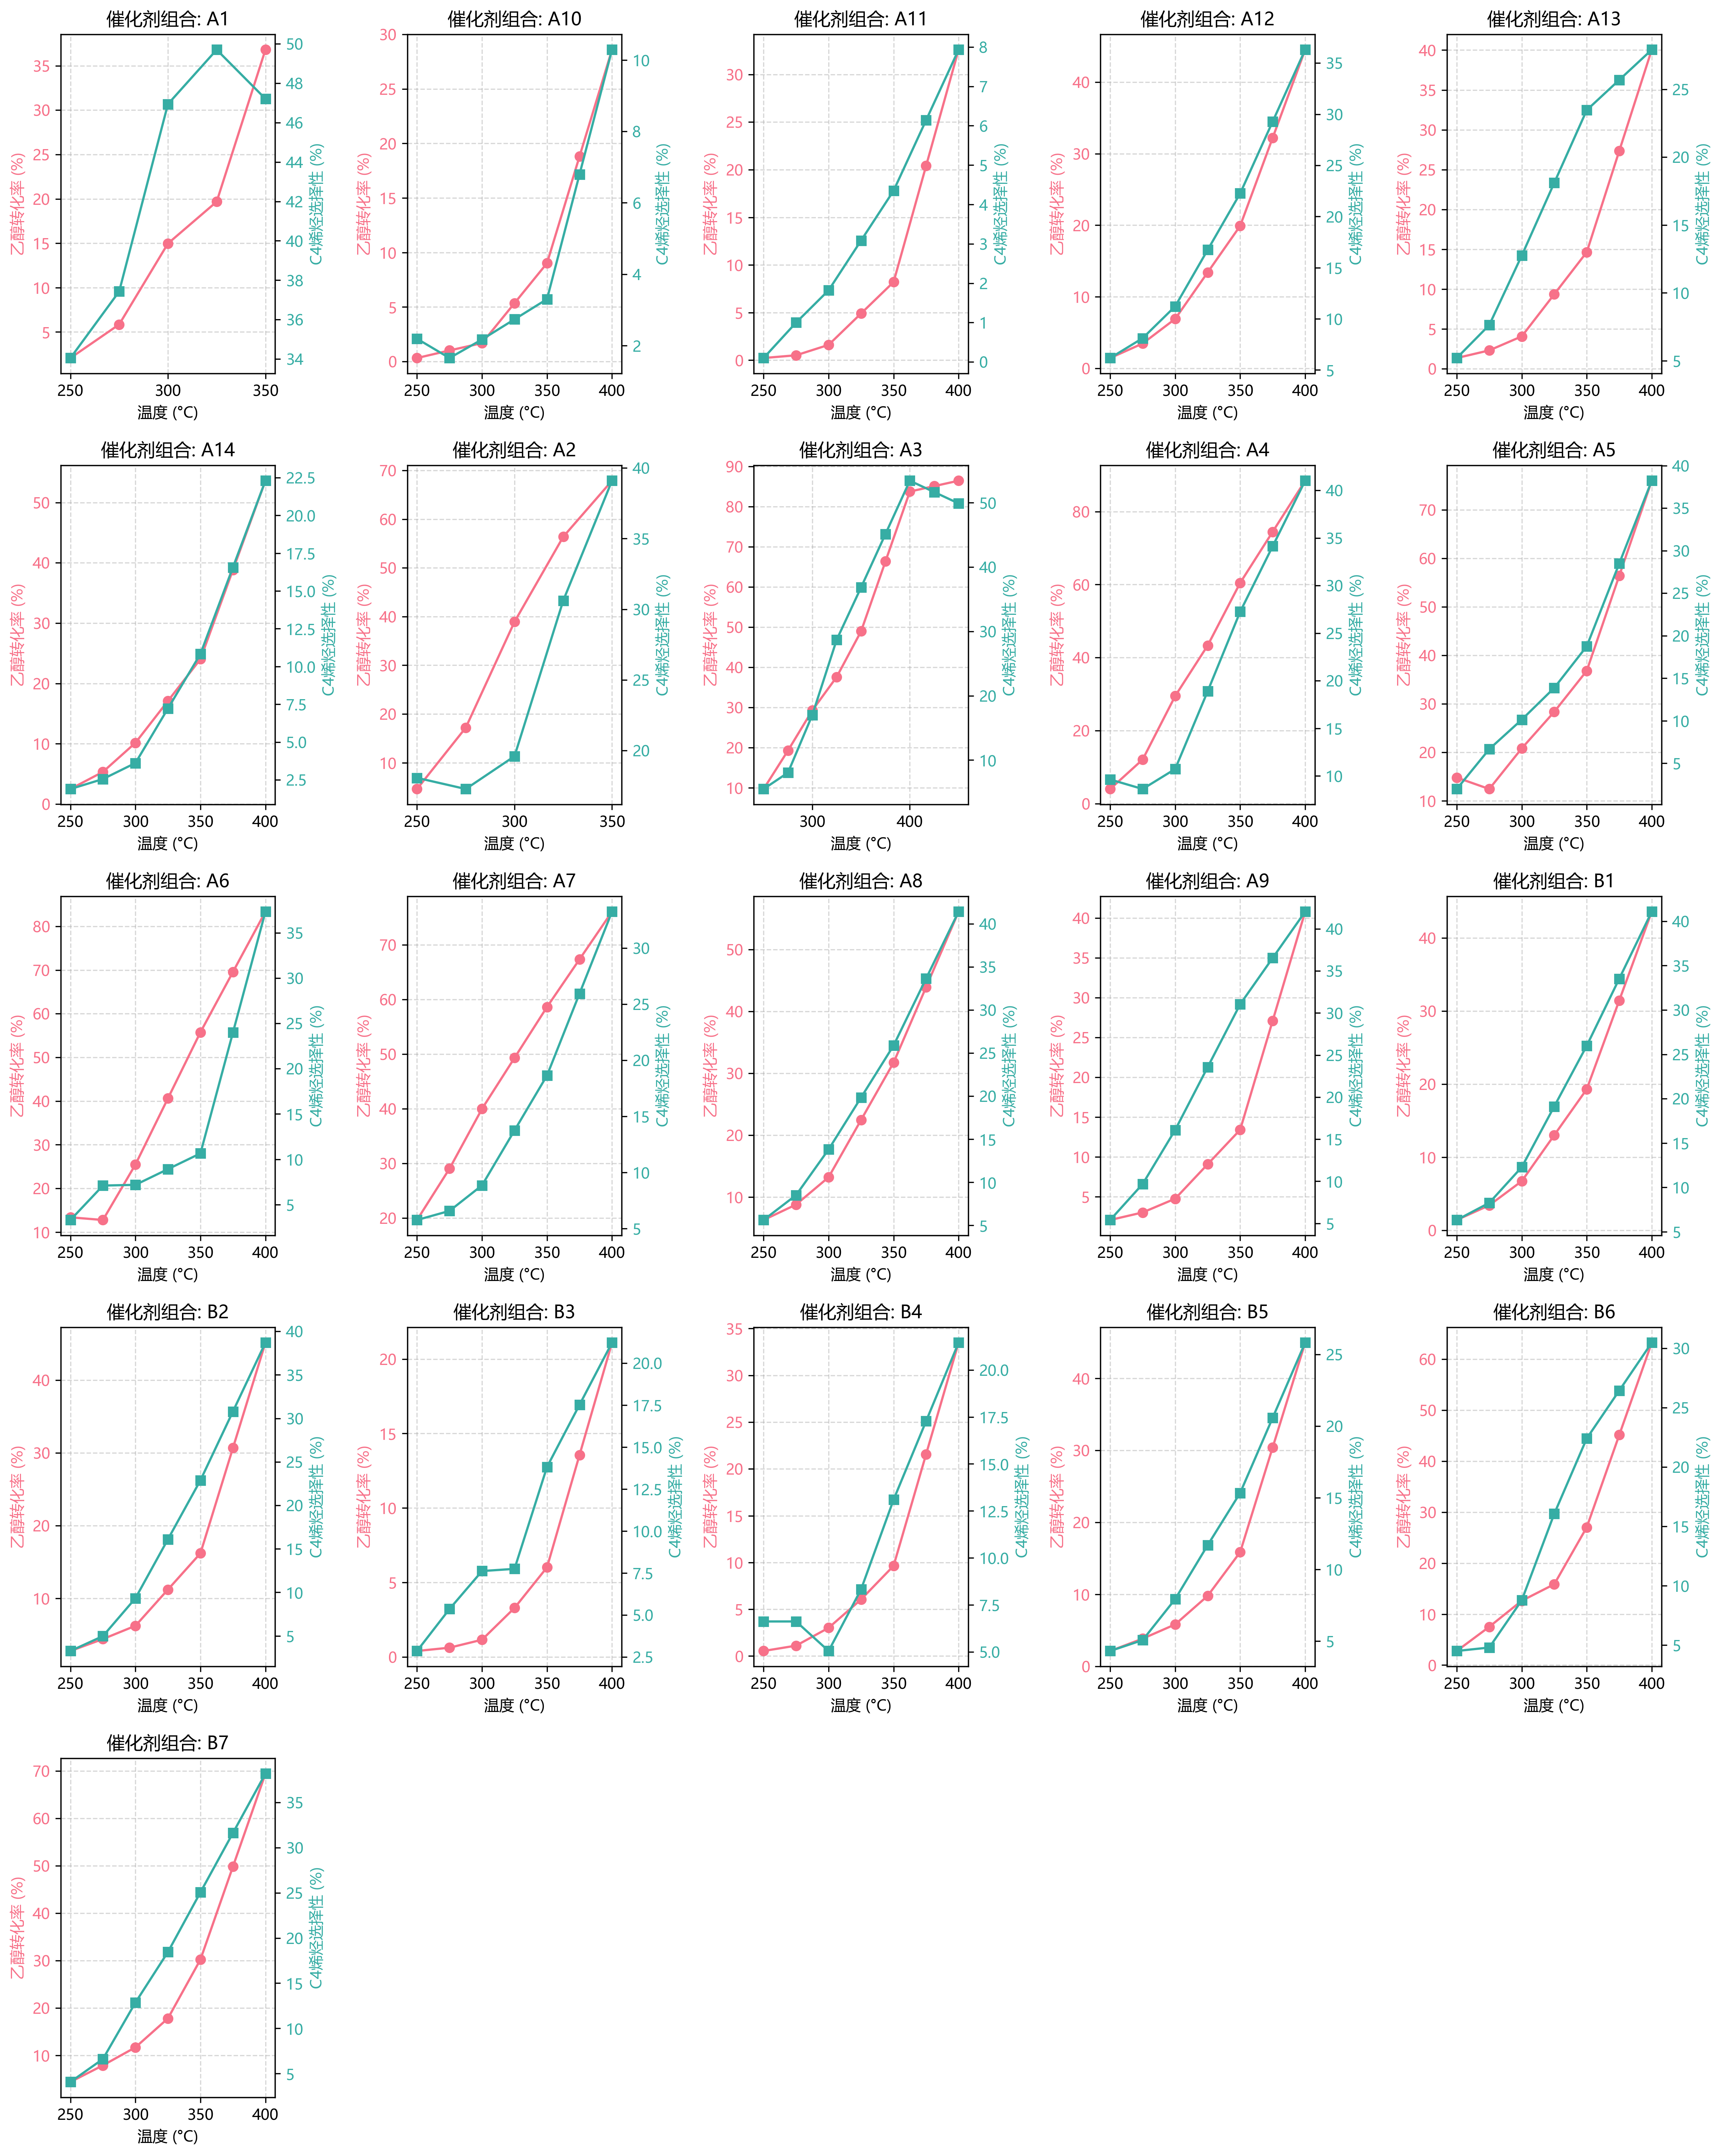
\includegraphics [scale=0.4]{图/1-1-1.png}
	\caption{乙醇转化率和C4烯烃选择性与温度的关系} 
	\label{fig:1}
\end{figure}

\begin{table}[!htbp]
	\caption{催化剂组合在不同温度下的乙醇转化率与C4烯烃选择性相关系数(部分)}
	\centering
	\begin{tabular}{c c c}
		\hline
		\multicolumn{1}{c}{催化剂组合} & \multicolumn{1}{c}{乙醇转化率-温度 (r)} & \multicolumn{1}{c}{C4烯烃选择性-温度 (r)} \\
		\hline
		A1  & 0.9655 & 0.8871 \\
		A2  & 0.9950 & 0.9143 \\
		B1  & 0.9621 & 0.9858 \\
		B2  & 0.9293 & 0.9848 \\
		\hline
	\end{tabular}
	\label{tab:1}
\end{table}

\begin{figure}[h]%[h]:固定作用
	\centering%置中
	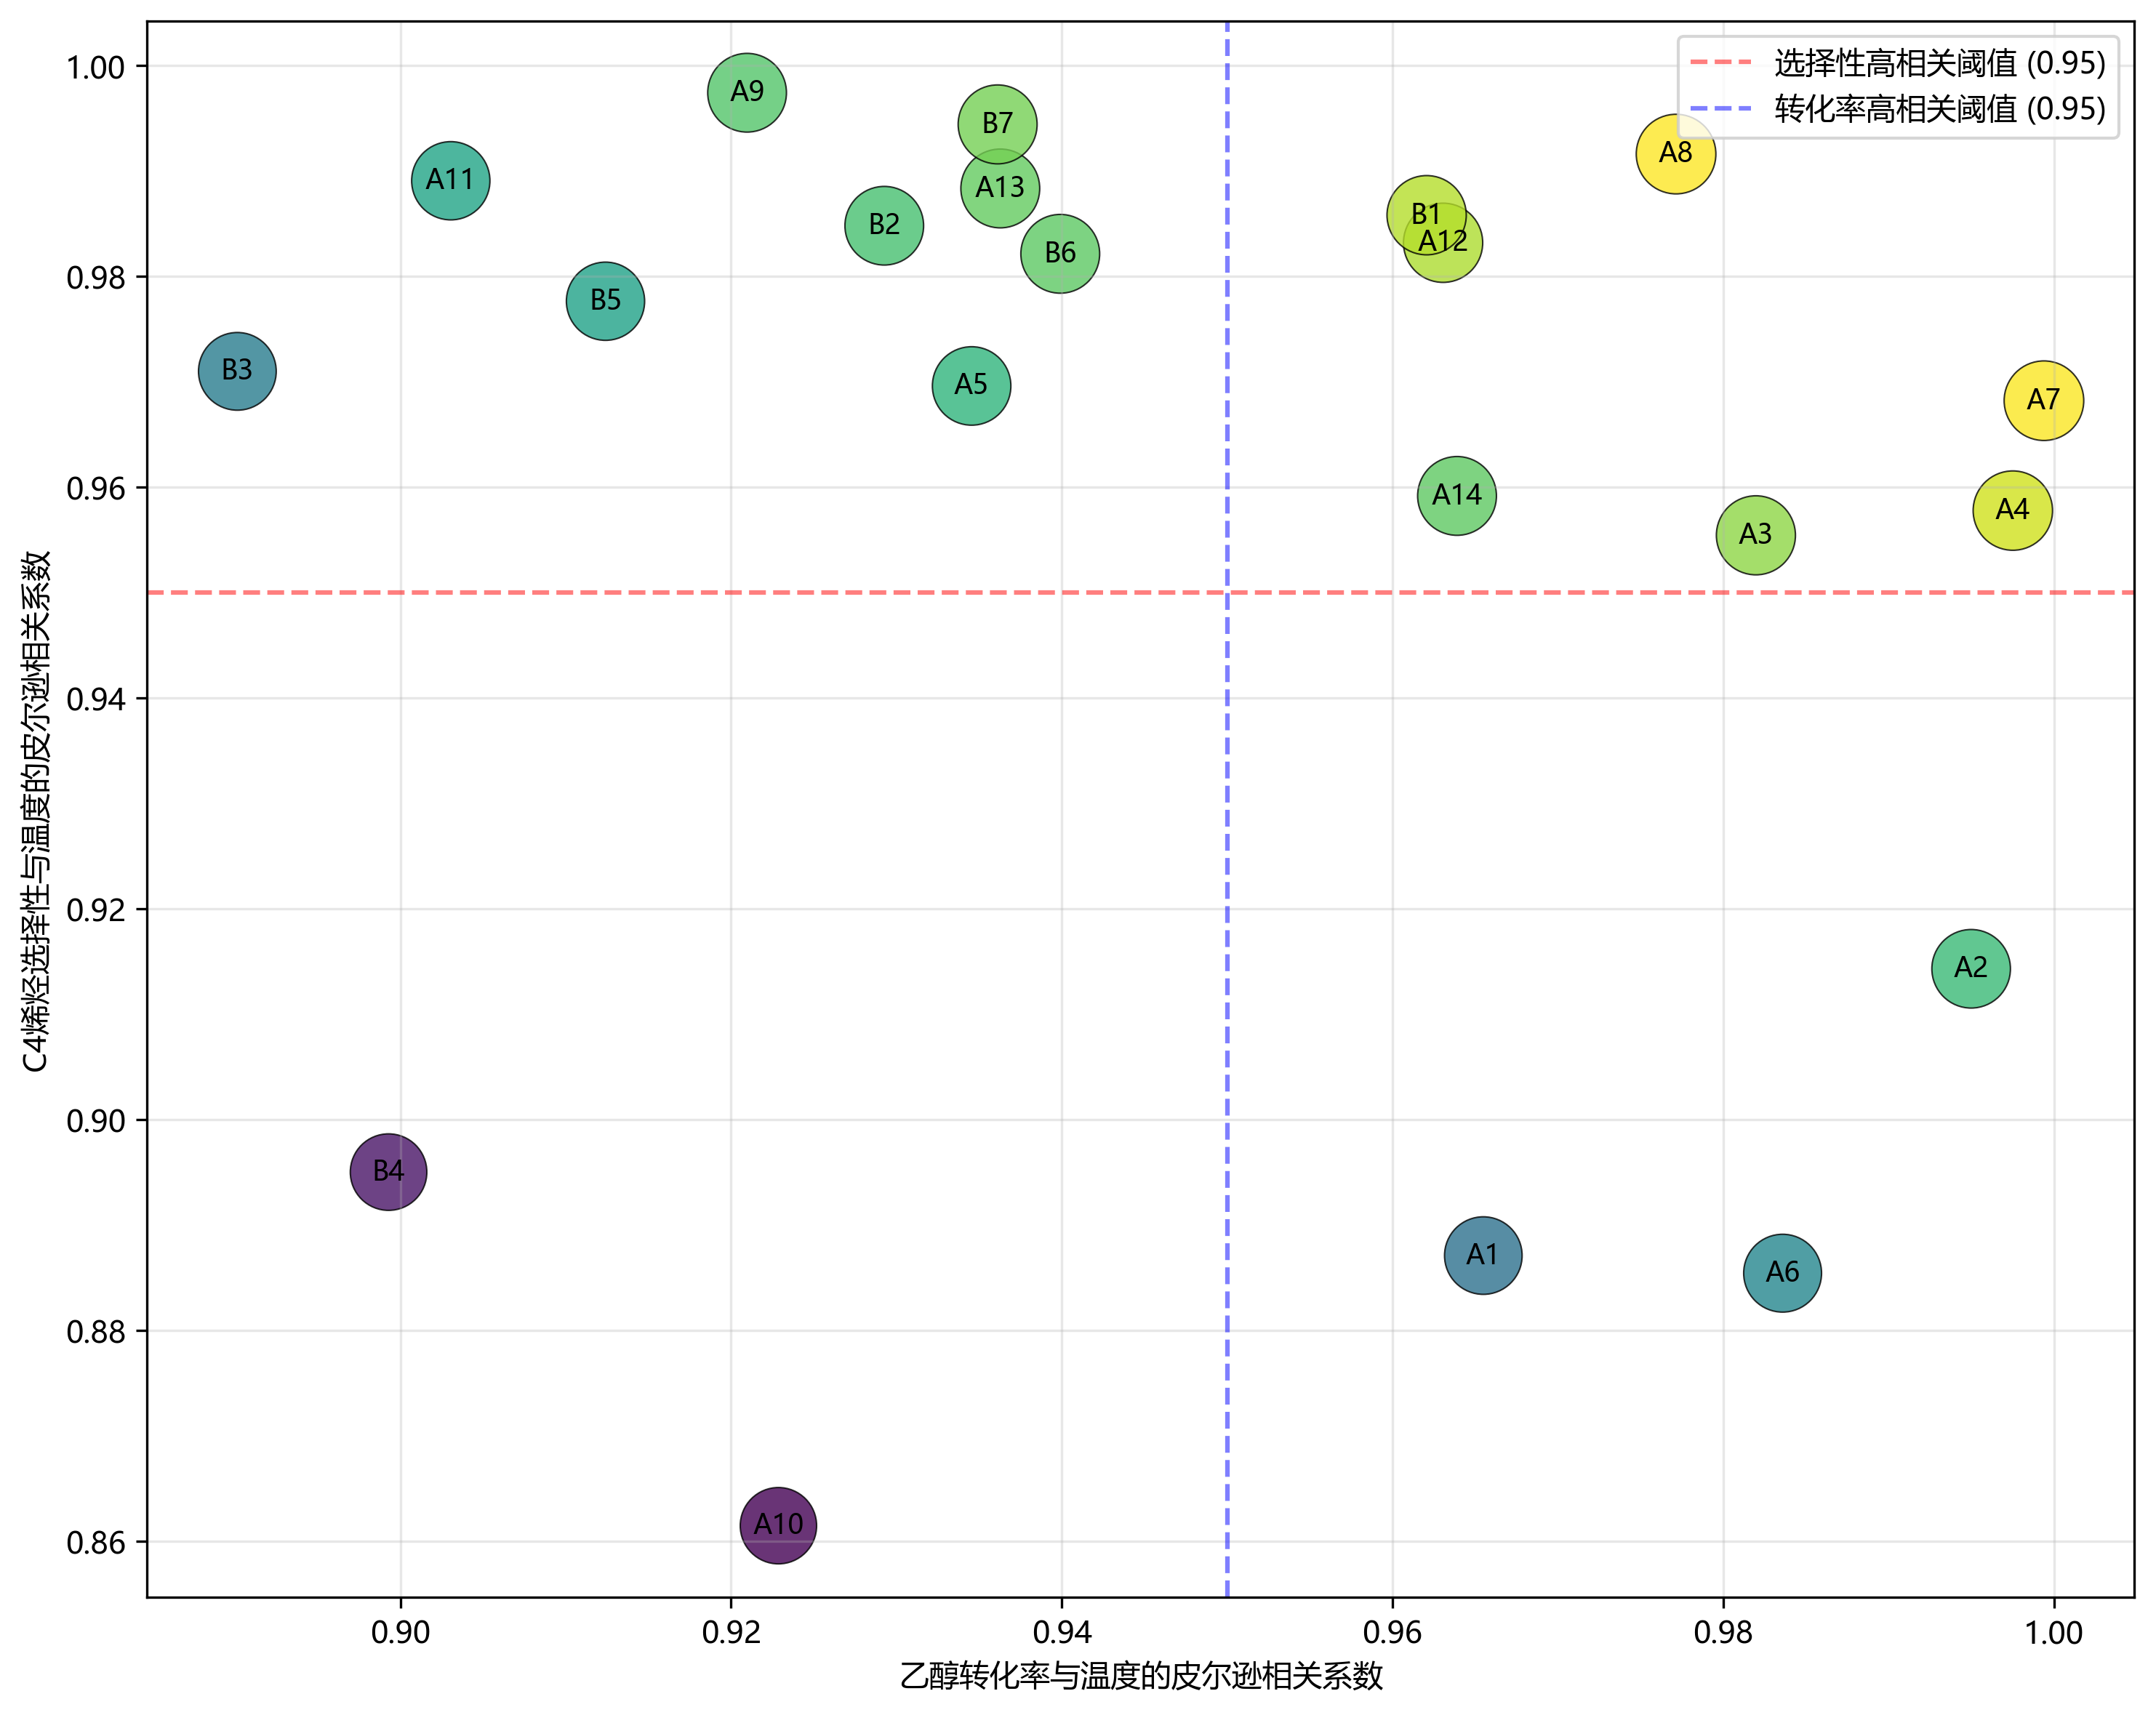
\includegraphics [scale=0.6]{图/1-2-2.png}
	\caption{各催化剂组合双指标相关性分布} 
	\label{fig:1}
\end{figure}

\begin{figure}[h]%[h]:固定作用
	\centering%置中
	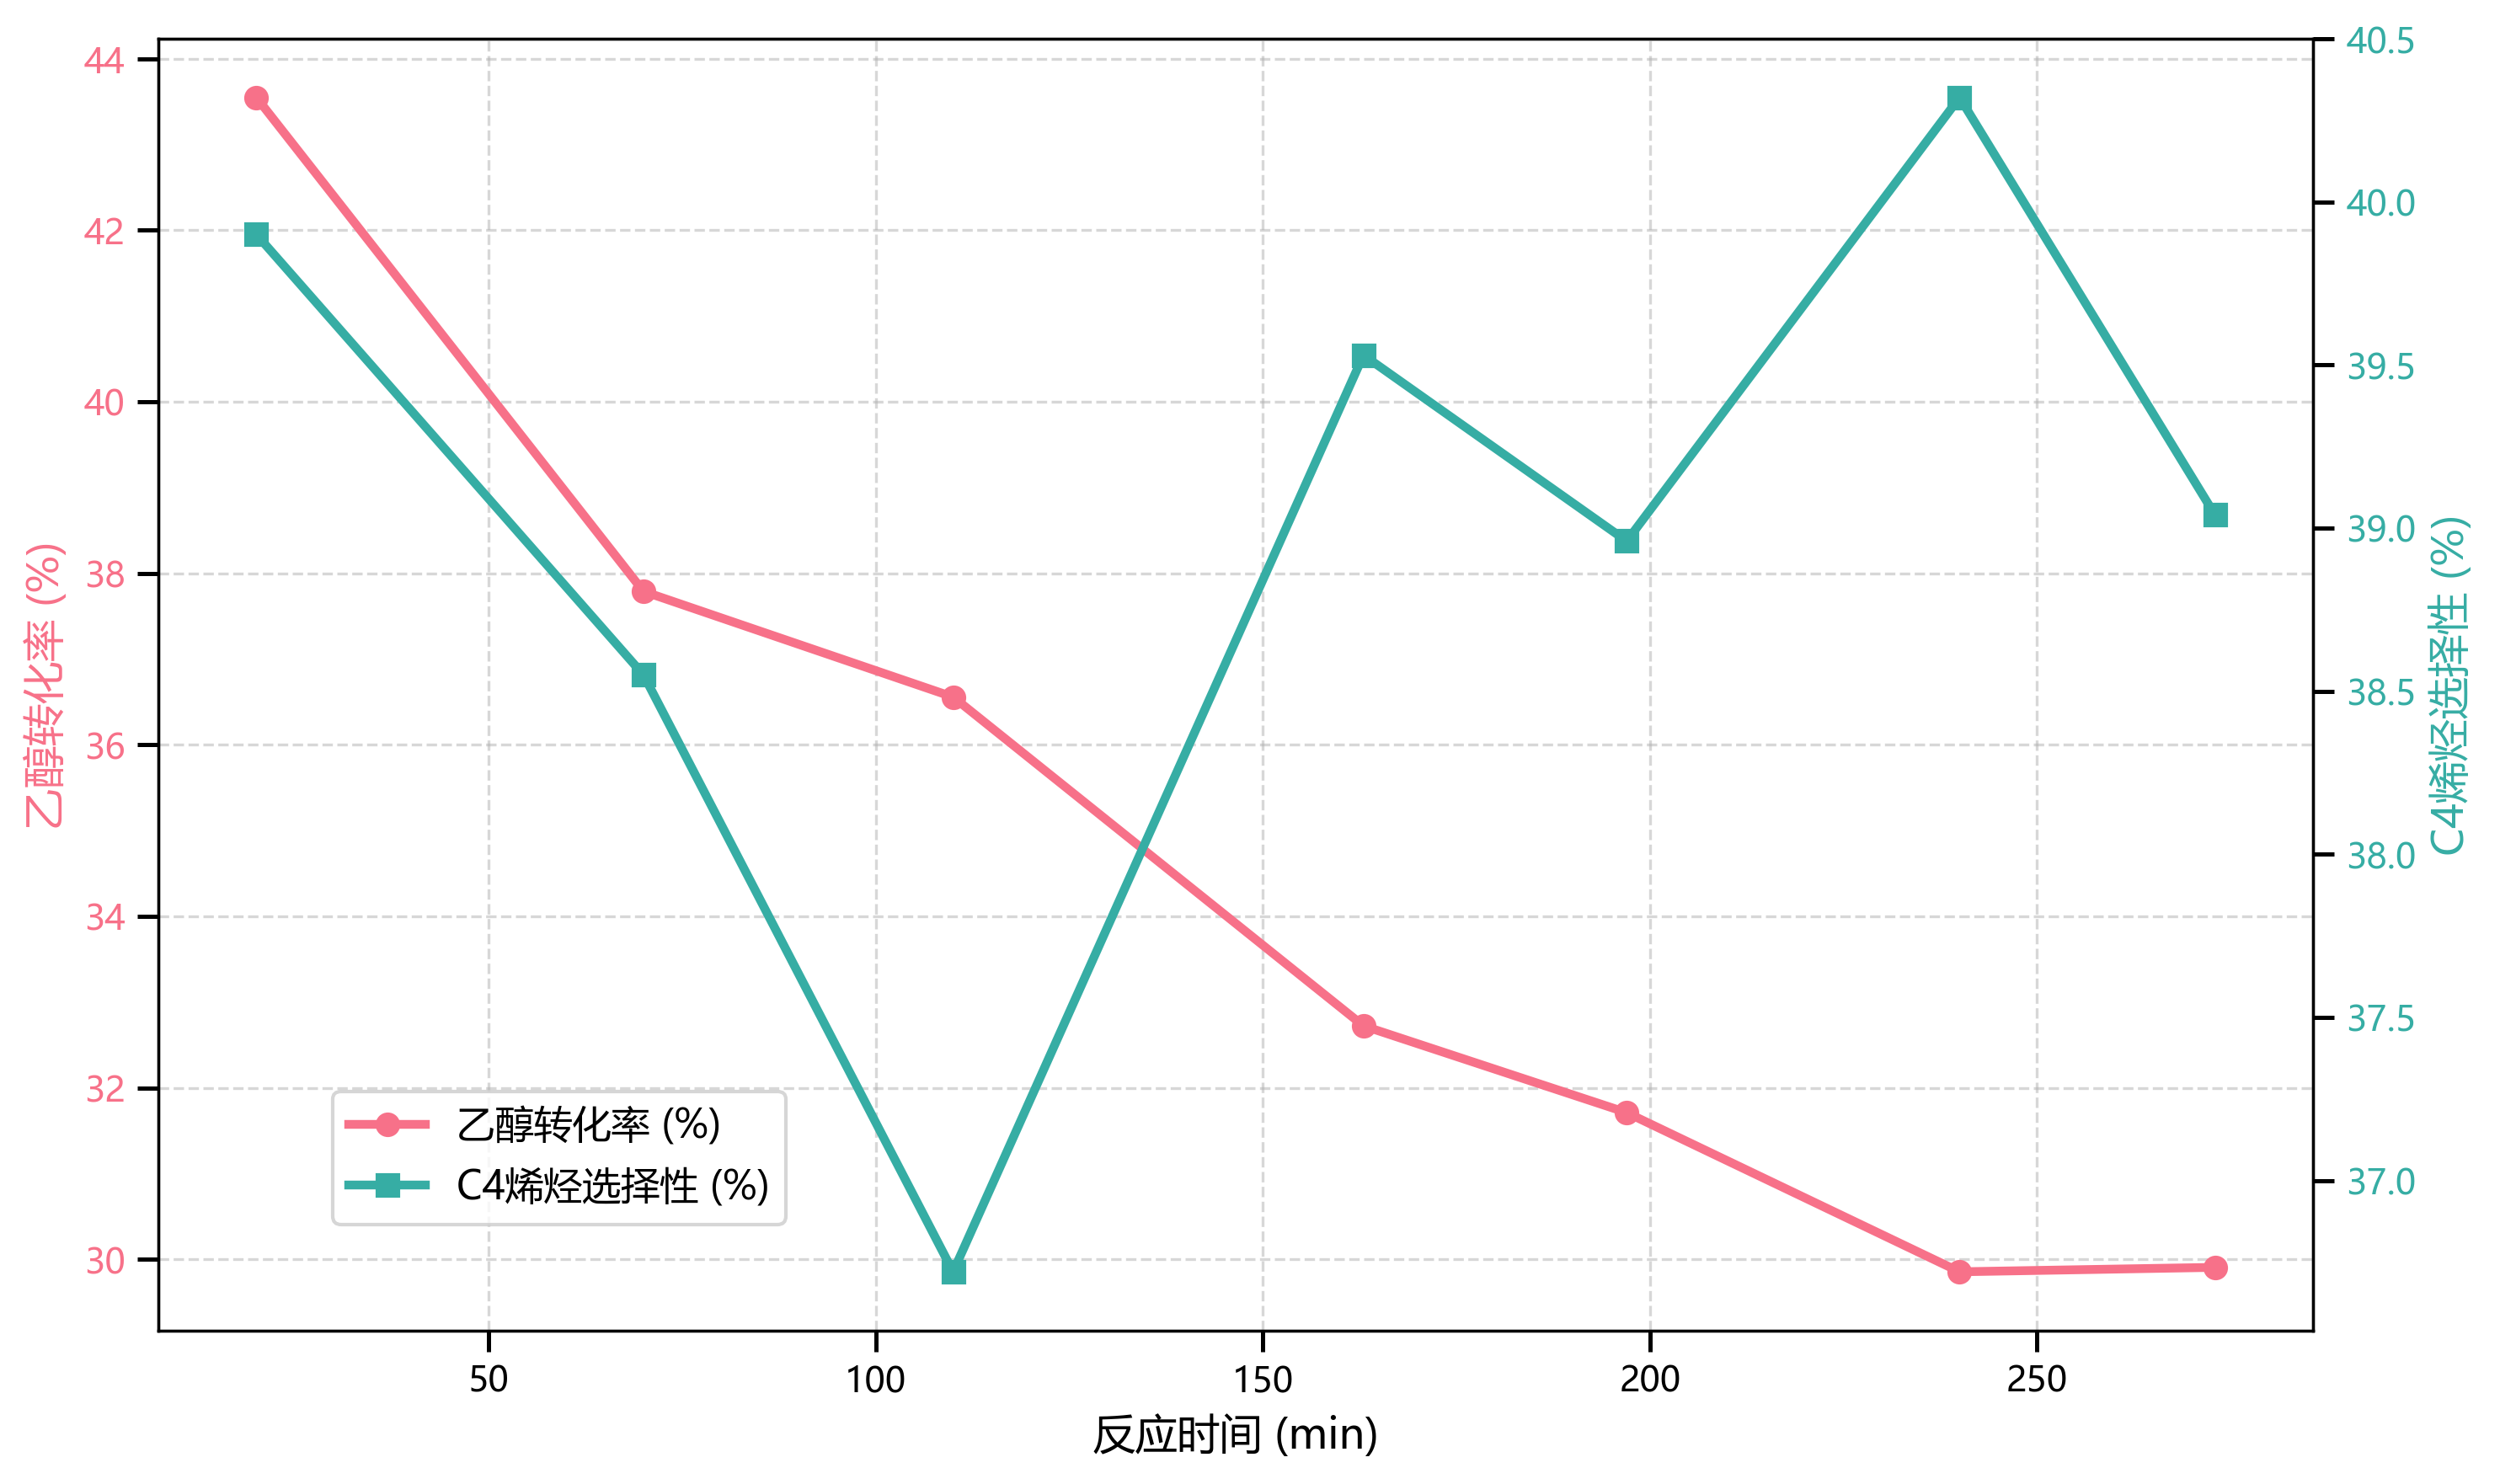
\includegraphics [scale=0.6]{图/1-2-1.png}
	\caption{350°C 下催化剂组合稳定性测试(不同反应时间性能变化)} 
	\label{fig:1}
\end{figure}

\newpage

\subsection*{问题二详细数据表}

\begin{figure}[h]%[h]:固定作用
	\centering%置中
	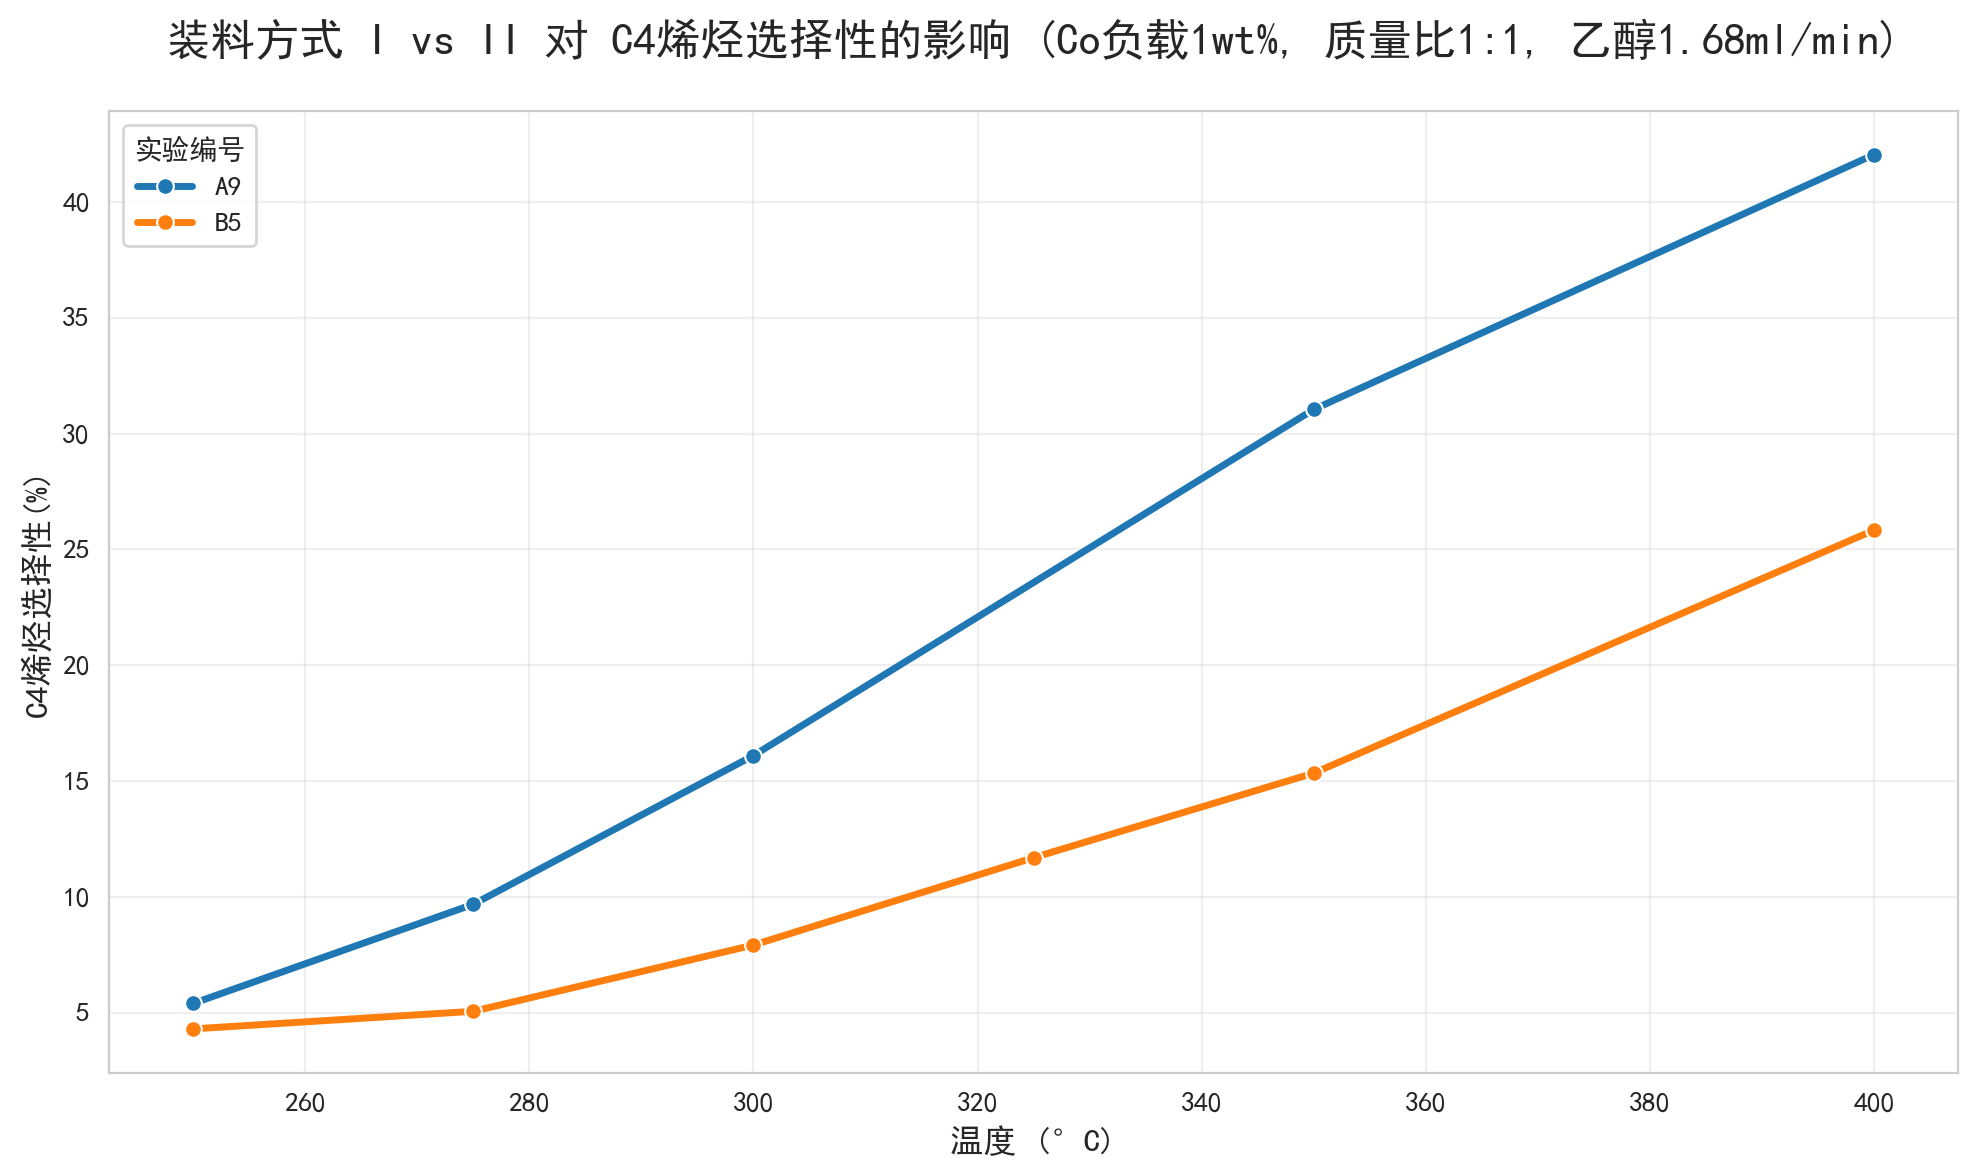
\includegraphics [scale=0.6]{图/2-1-2-1.png}
	\caption{装料方式对C4烯烃选择性的影响(Co负载1wt\%,质量比1:1,乙醇1.68ml/min)} 
	\label{fig:1}
\end{figure}

\newpage

\begin{figure}[h]%[h]:固定作用
	\centering%置中
	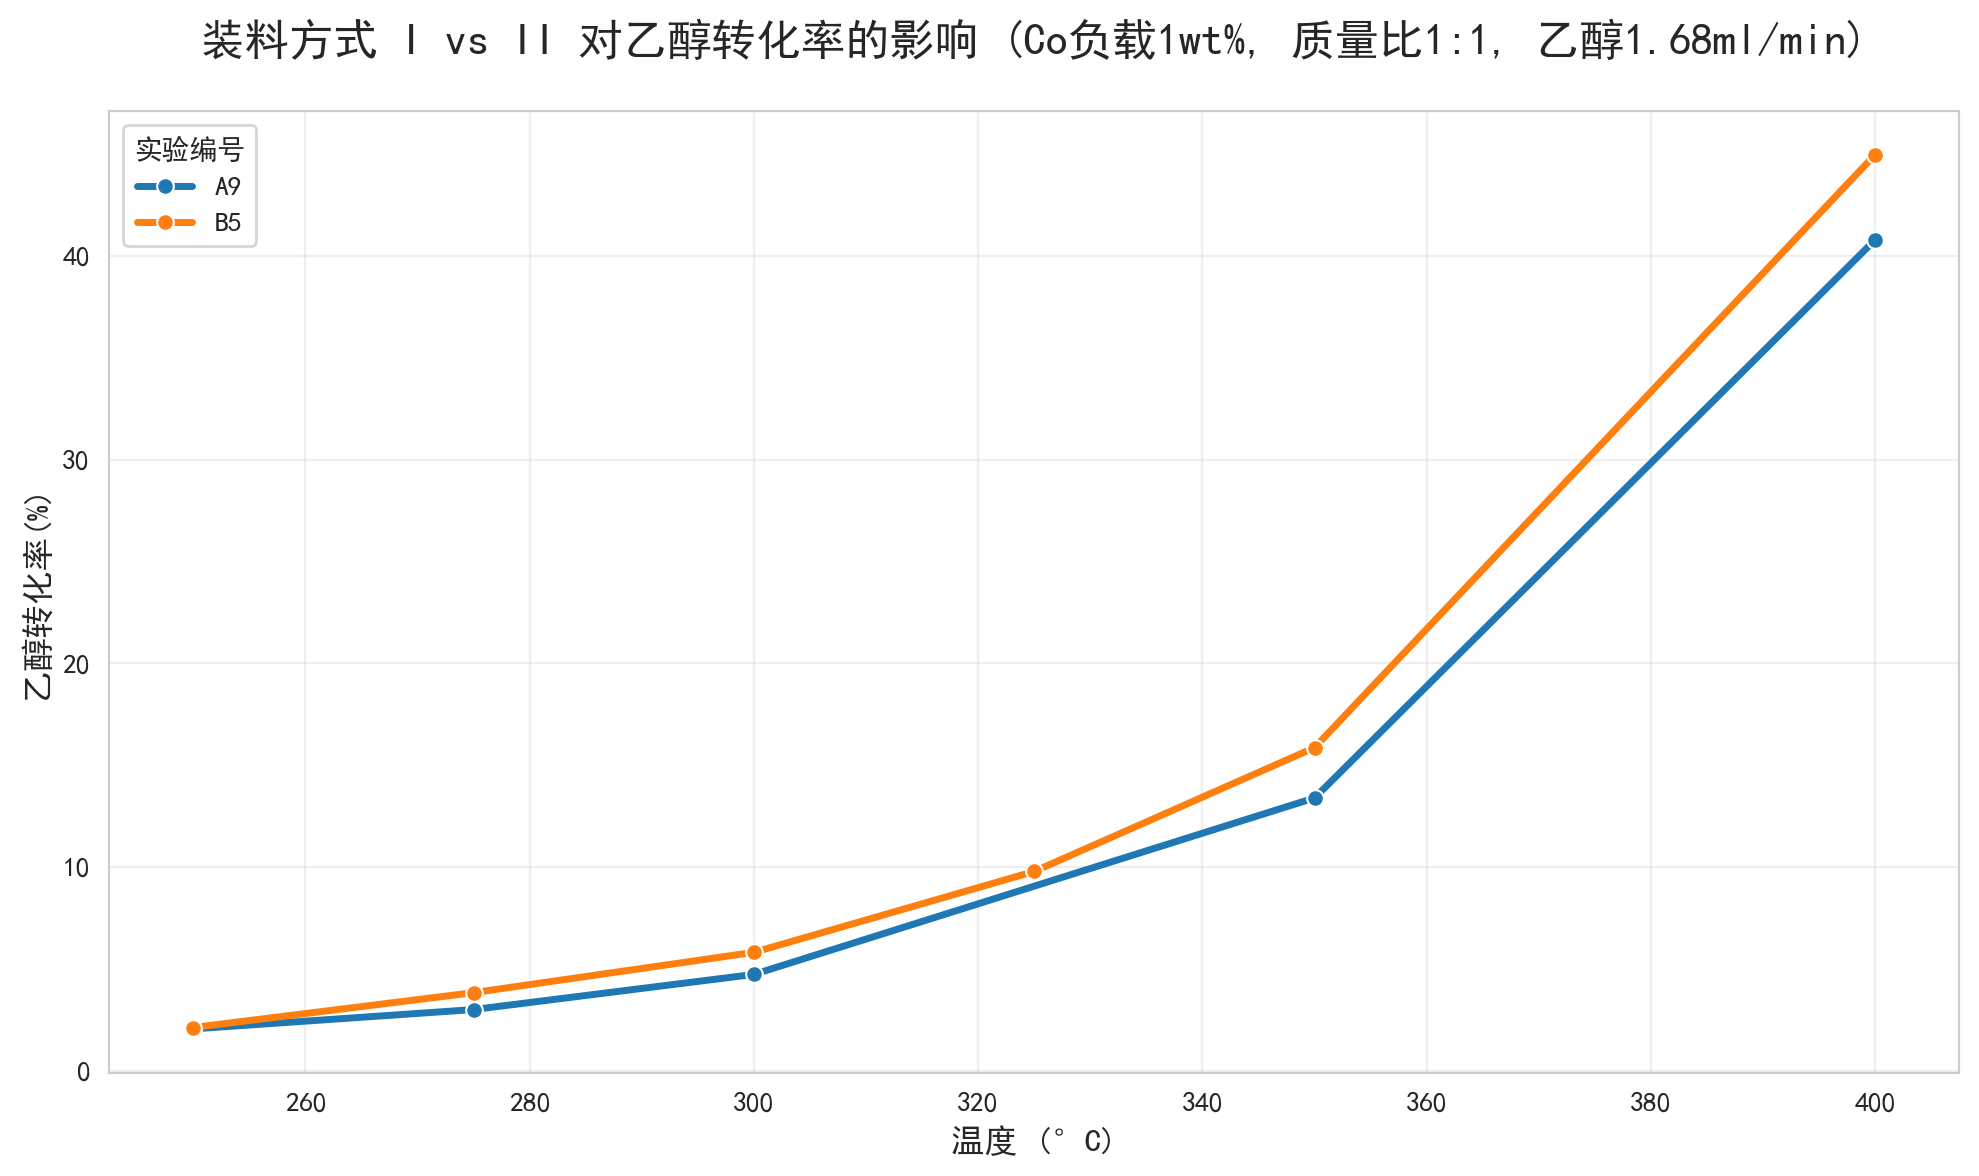
\includegraphics [scale=0.6]{图/2-1-2-2.png}
	\caption{装料方式对乙醇转化率的影响(Co负载1wt\%, 质量比1:1,乙醇1.68ml/min)} 
	\label{fig:1}
\end{figure}

\begin{figure}[h]%[h]:固定作用
	\centering%置中
	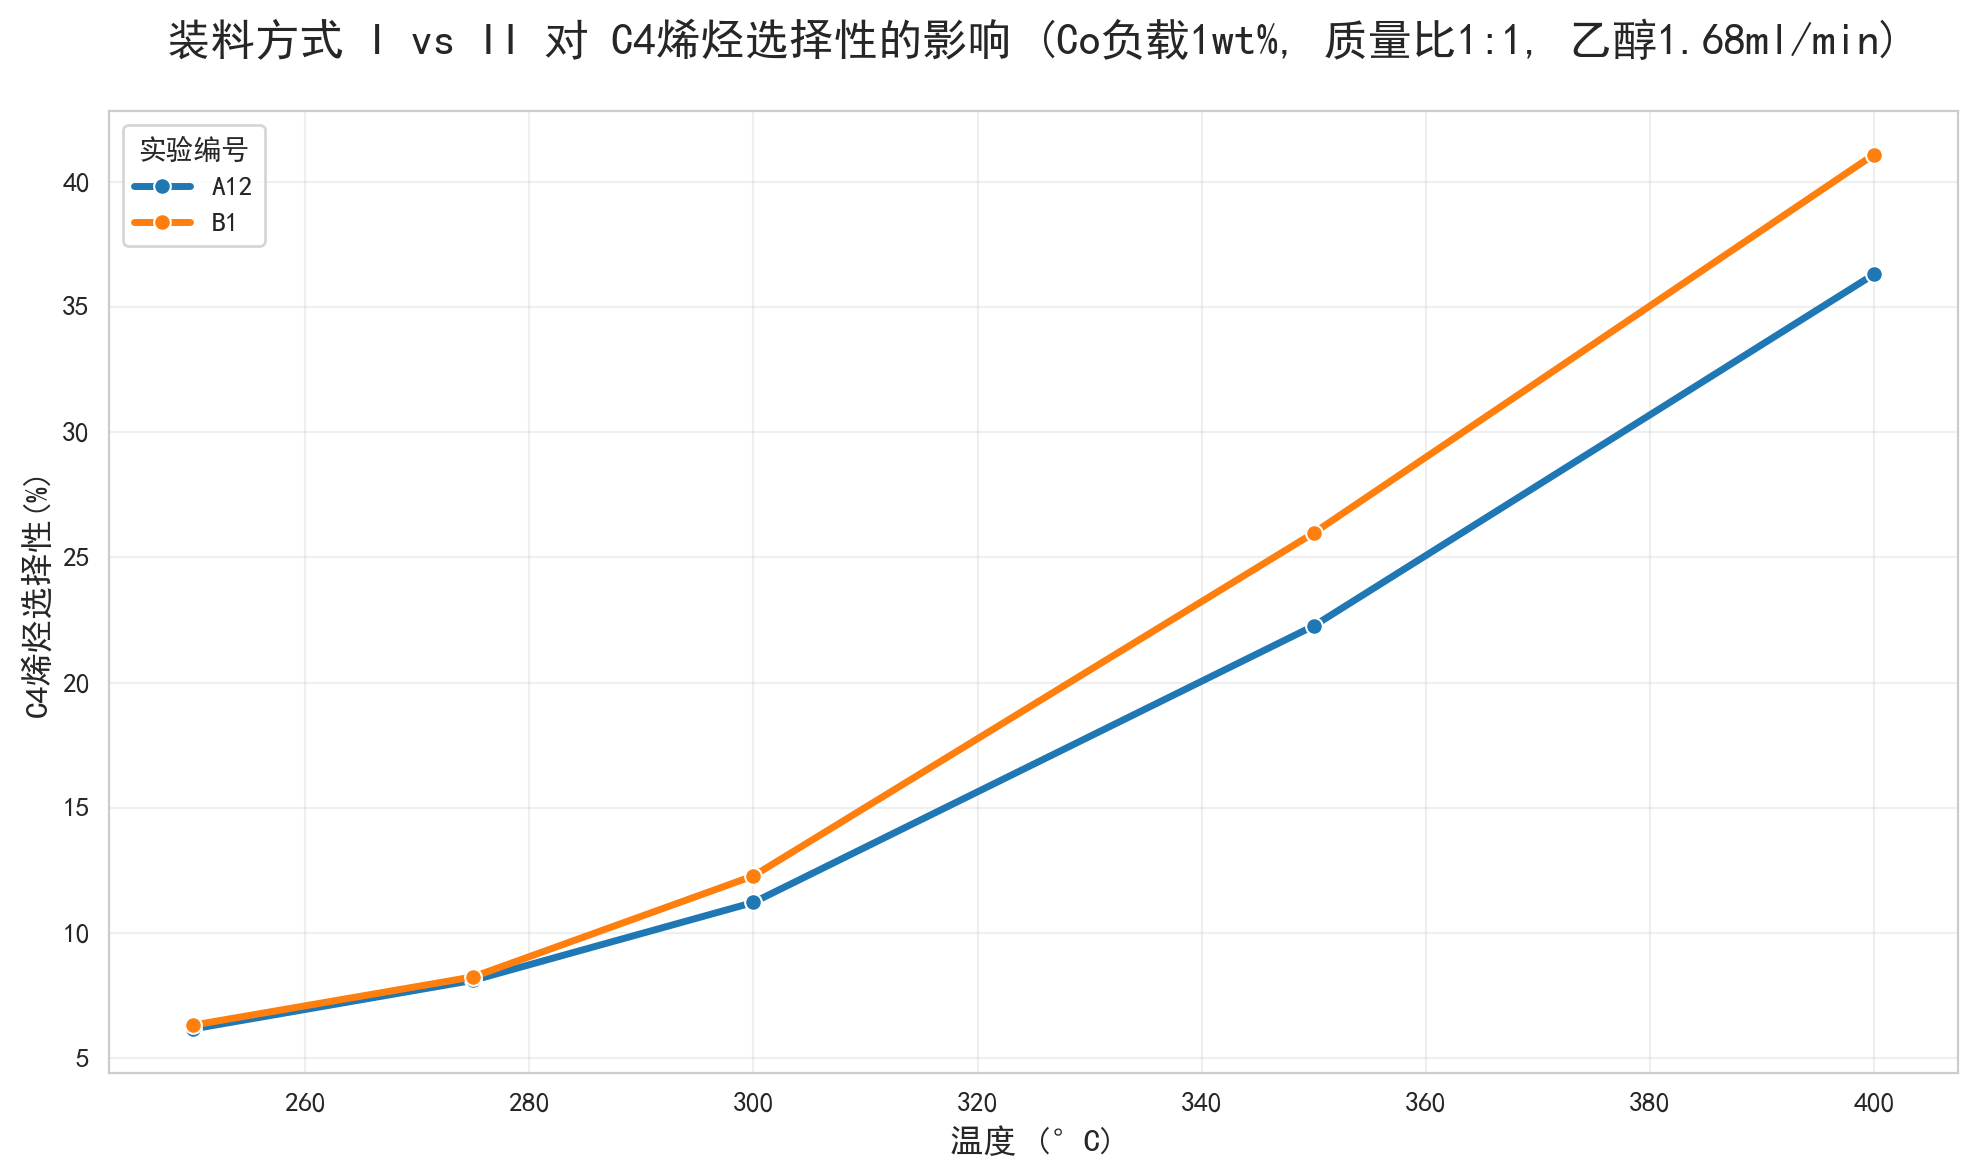
\includegraphics [scale=0.6]{图/2-1-1-1.png}
	\caption{装料方式 I vs II 对 C4烯烃选择性的影响 (Co负载1wt\%, 质量比1:1, 乙醇1.68ml/min)} 
	\label{fig:1}
\end{figure}

\begin{figure}[h]%[h]:固定作用
	\centering%置中
	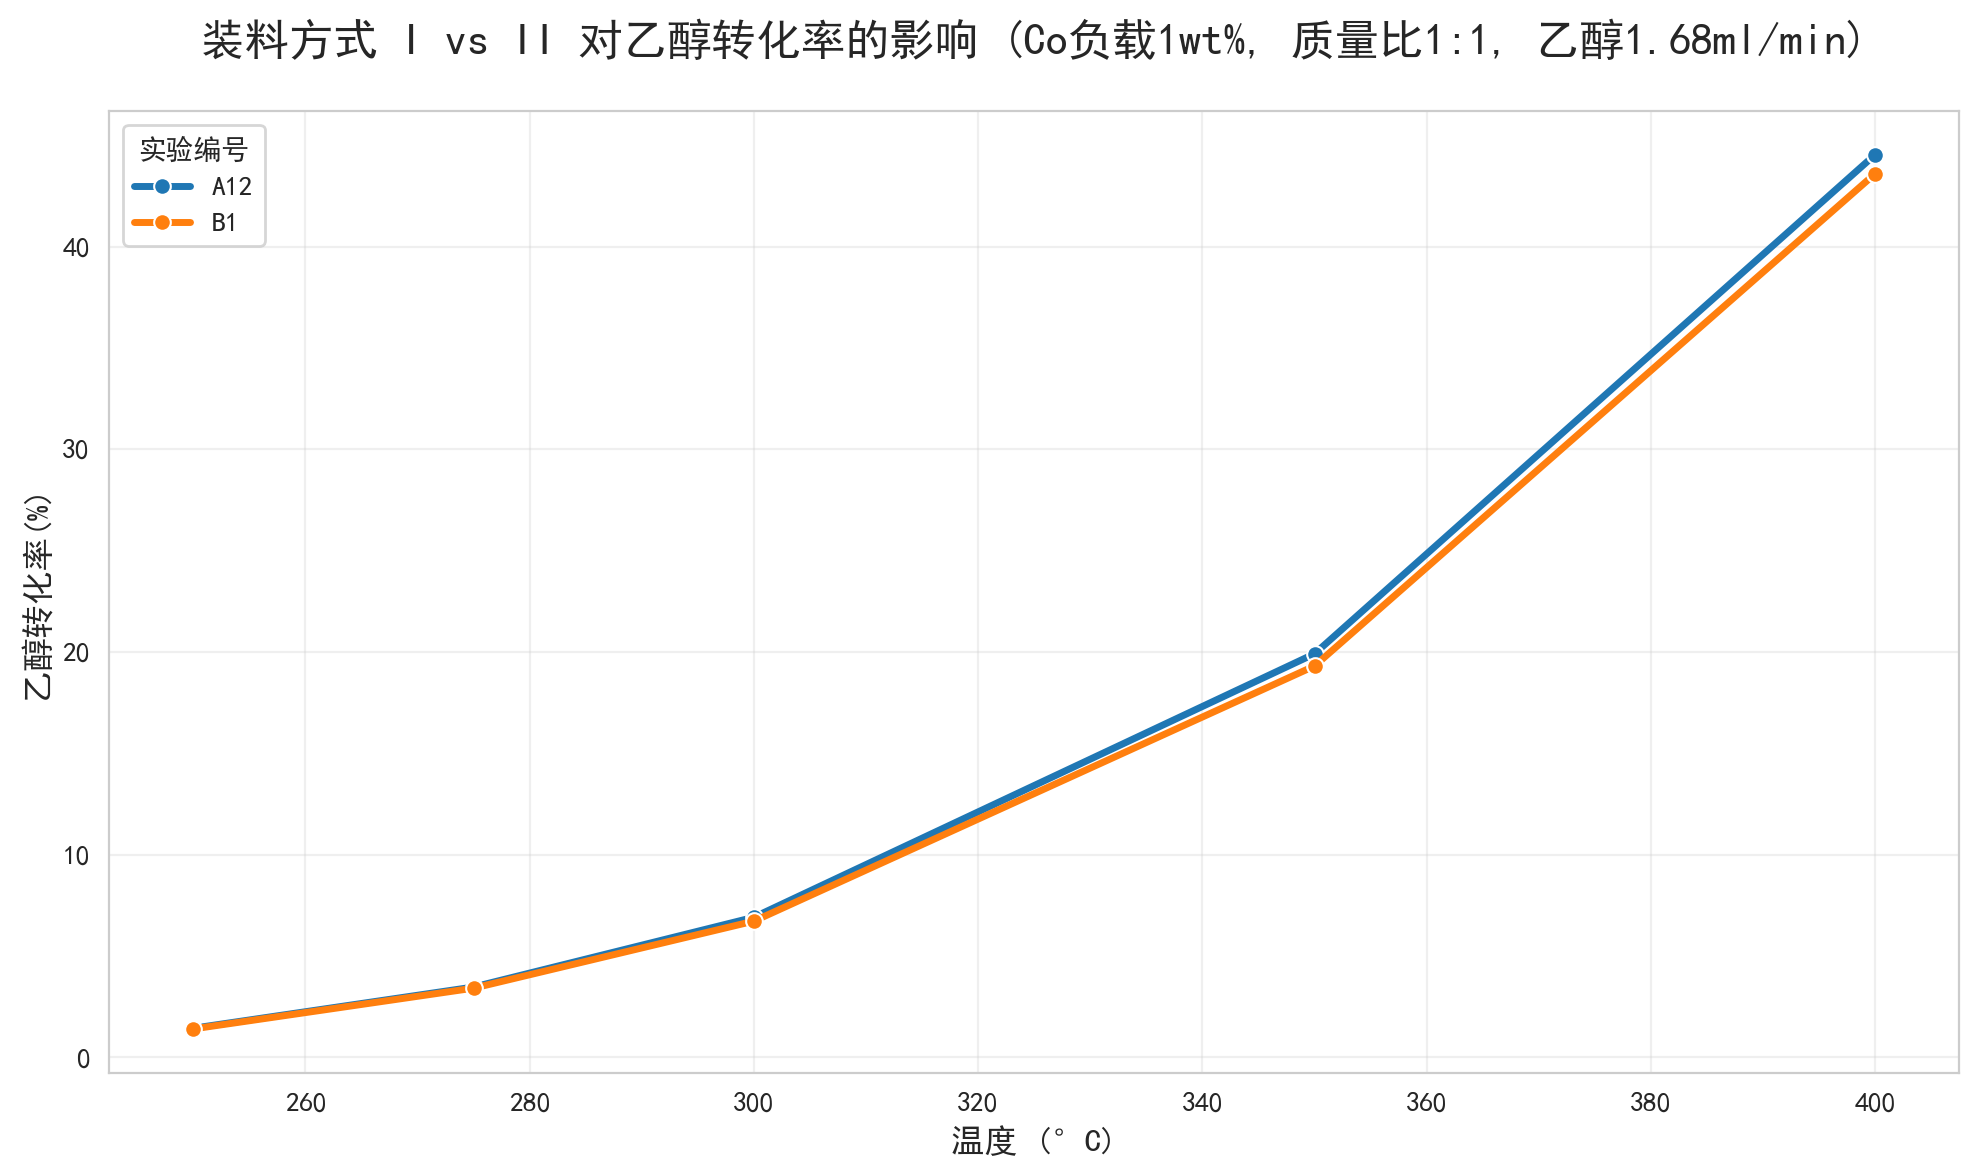
\includegraphics [scale=0.6]{图/2-1-1-2.png}
	\caption{装料方式 I vs II 对乙醇转化率的影响 (Co负载1wt\%, 质量比1:1, 乙醇1.68ml/min)} 
	\label{fig:1}
\end{figure}

\begin{figure}[h]%[h]:固定作用
	\centering%置中
	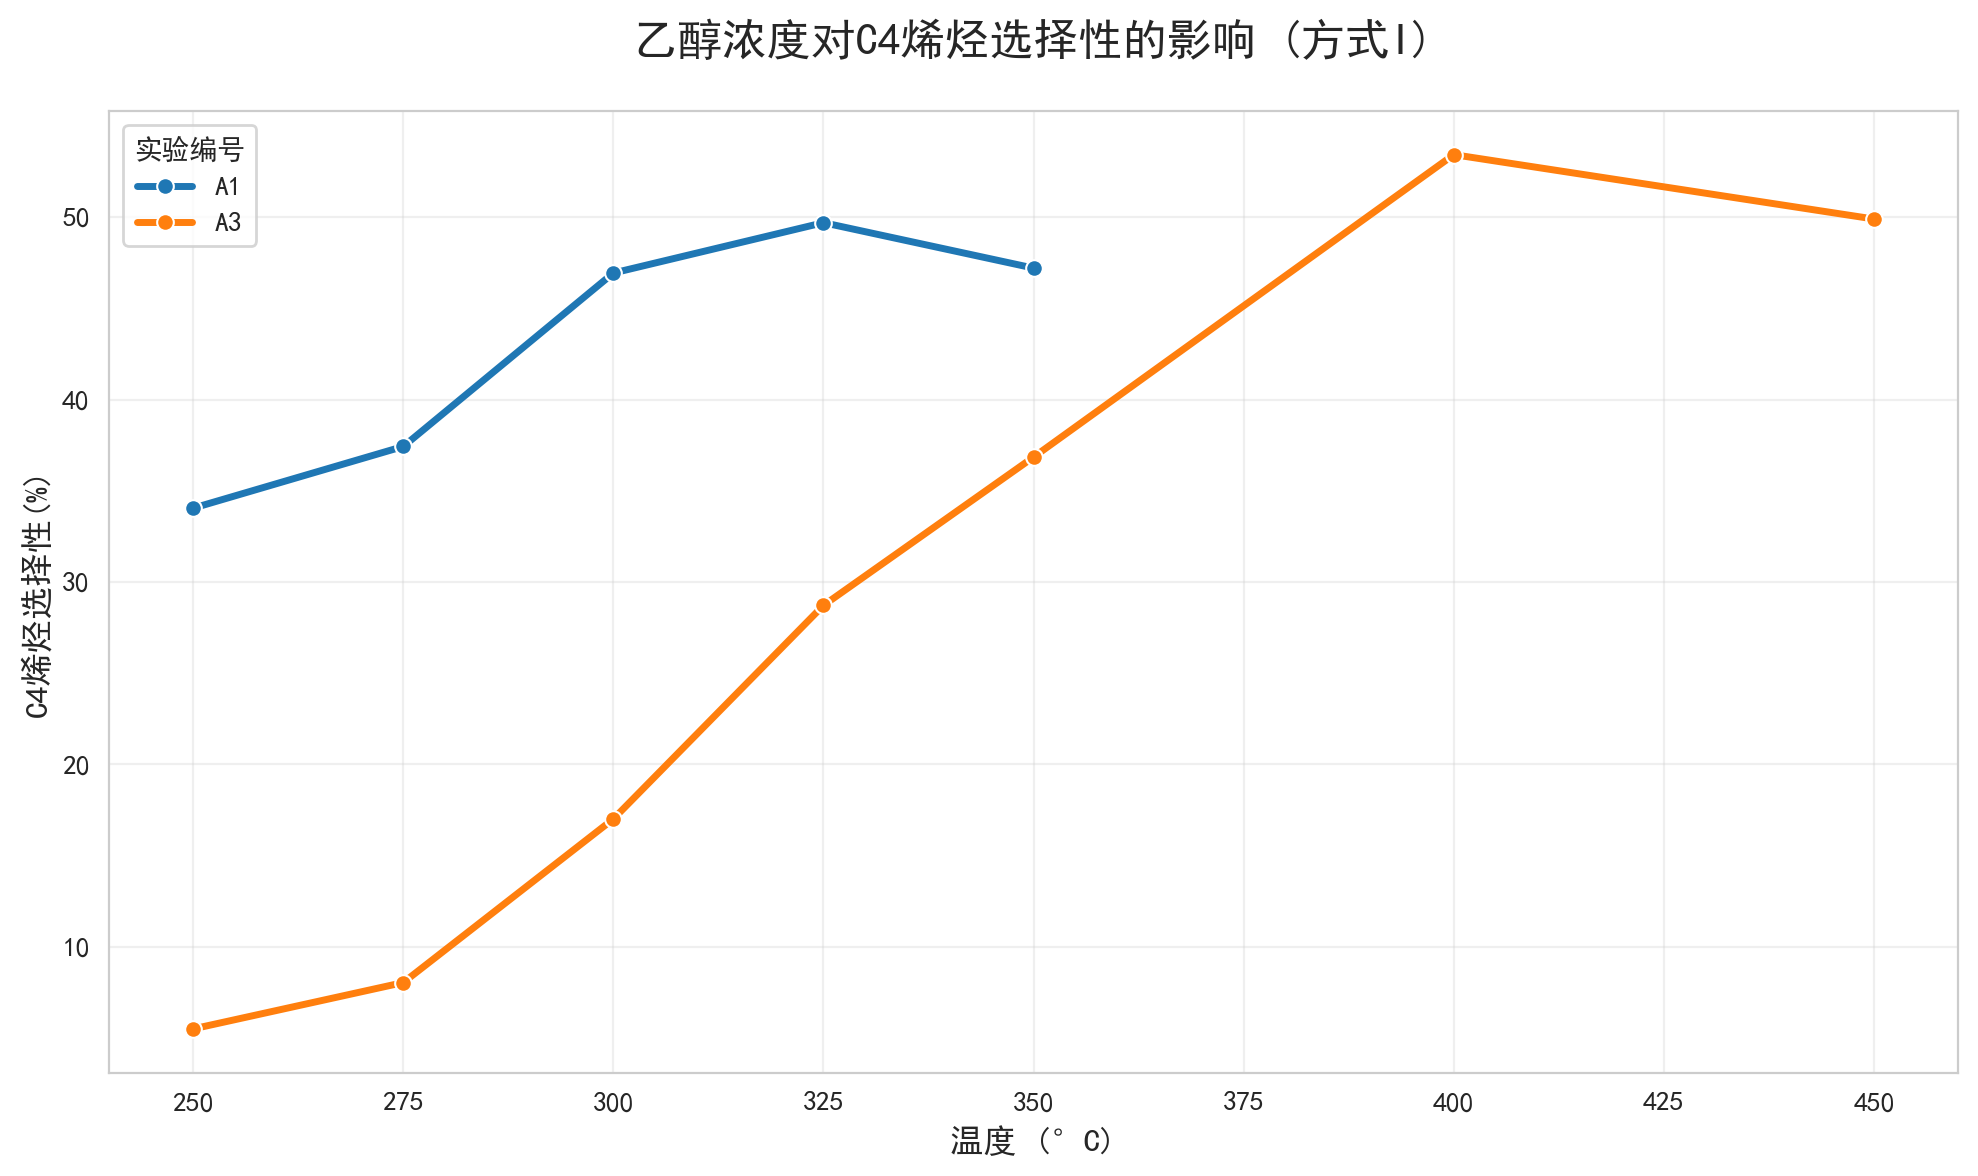
\includegraphics [scale=0.6]{图/2-2-1-1.png}
	\caption{乙醇浓度对C4烯烃选择性的影响 (方式I)} 
	\label{fig:1}
\end{figure}

\begin{figure}[h]%[h]:固定作用
	\centering%置中
	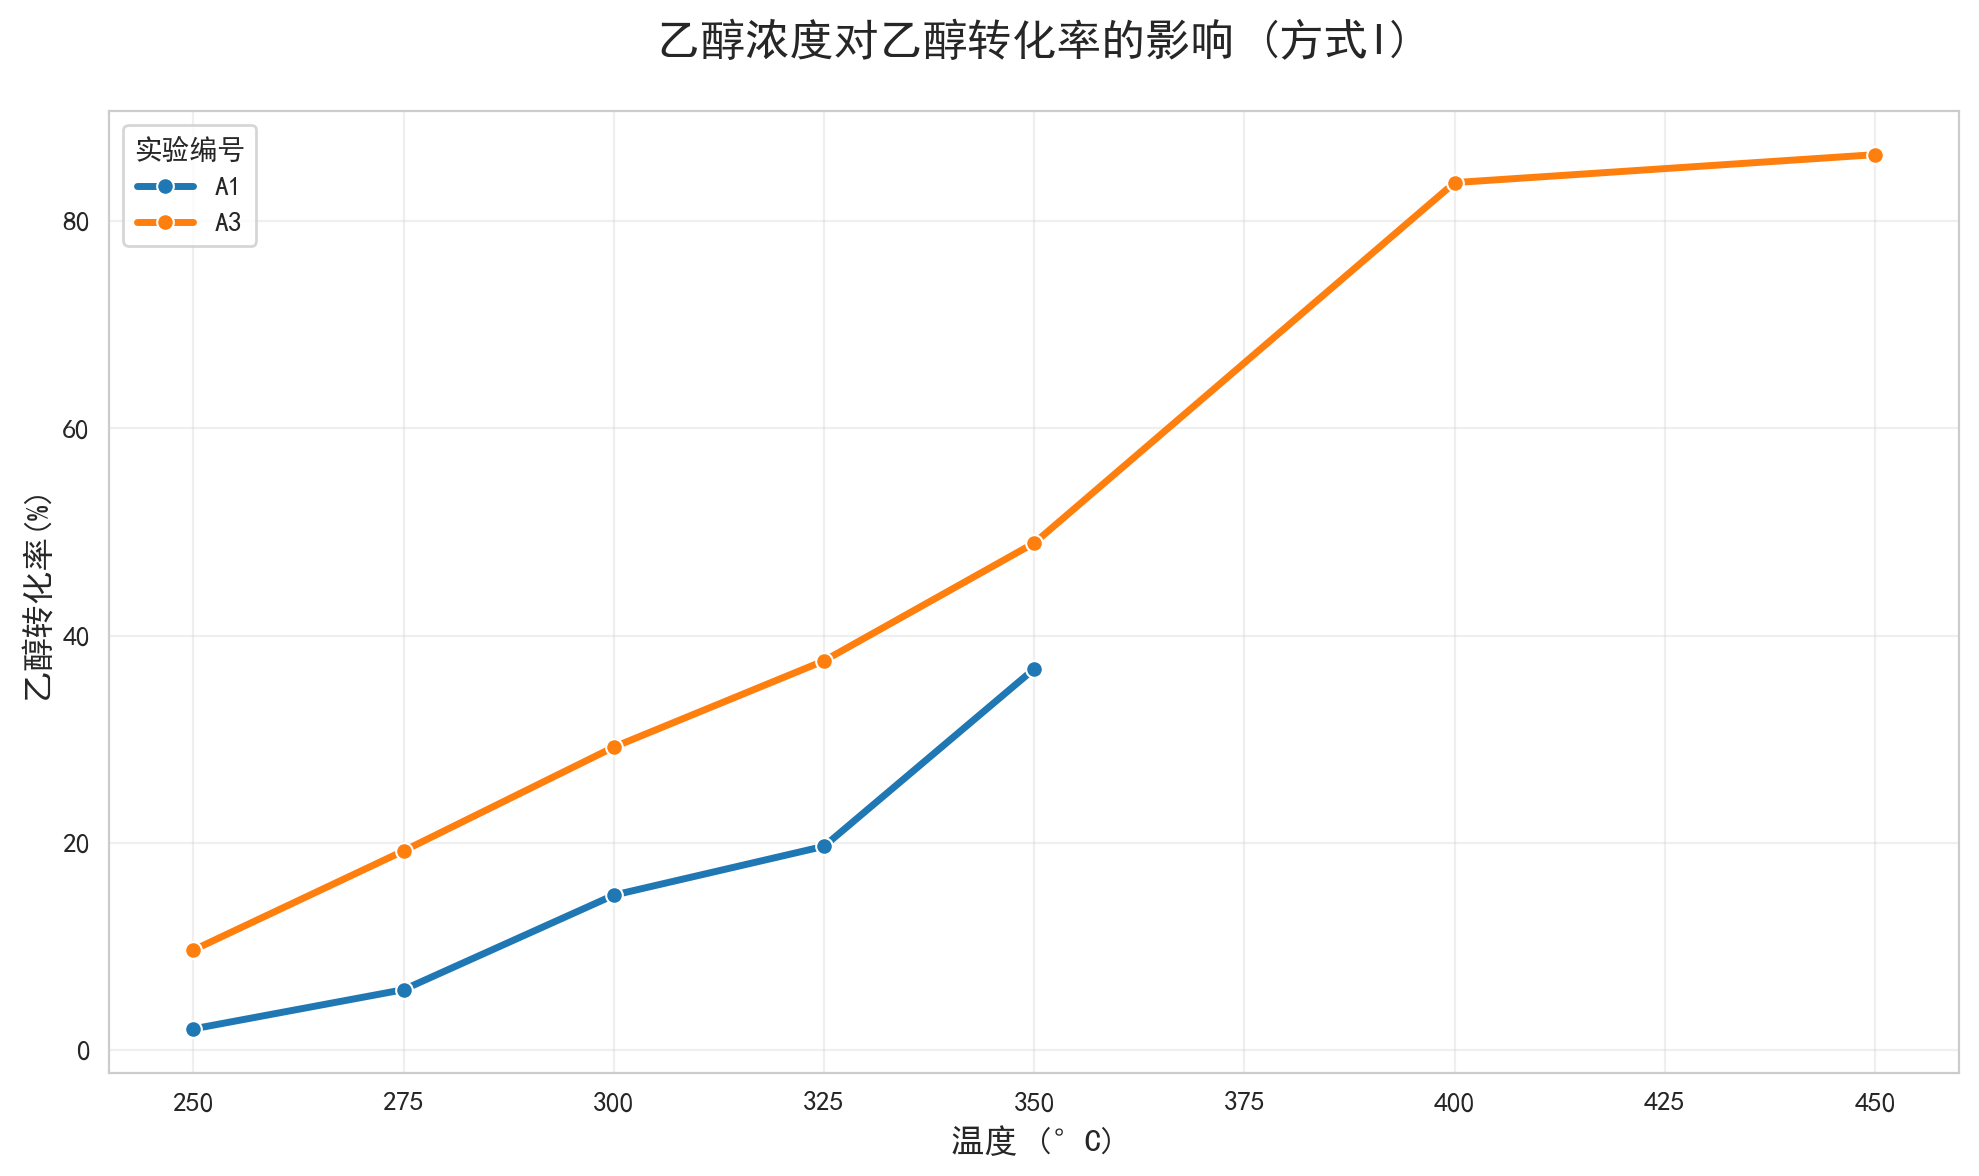
\includegraphics [scale=0.6]{图/2-2-1-2.png}
	\caption{乙醇浓度对乙醇转化率的影响 (方式I)} 
	\label{fig:1}
\end{figure}

\begin{figure}[h]%[h]:固定作用
	\centering%置中
	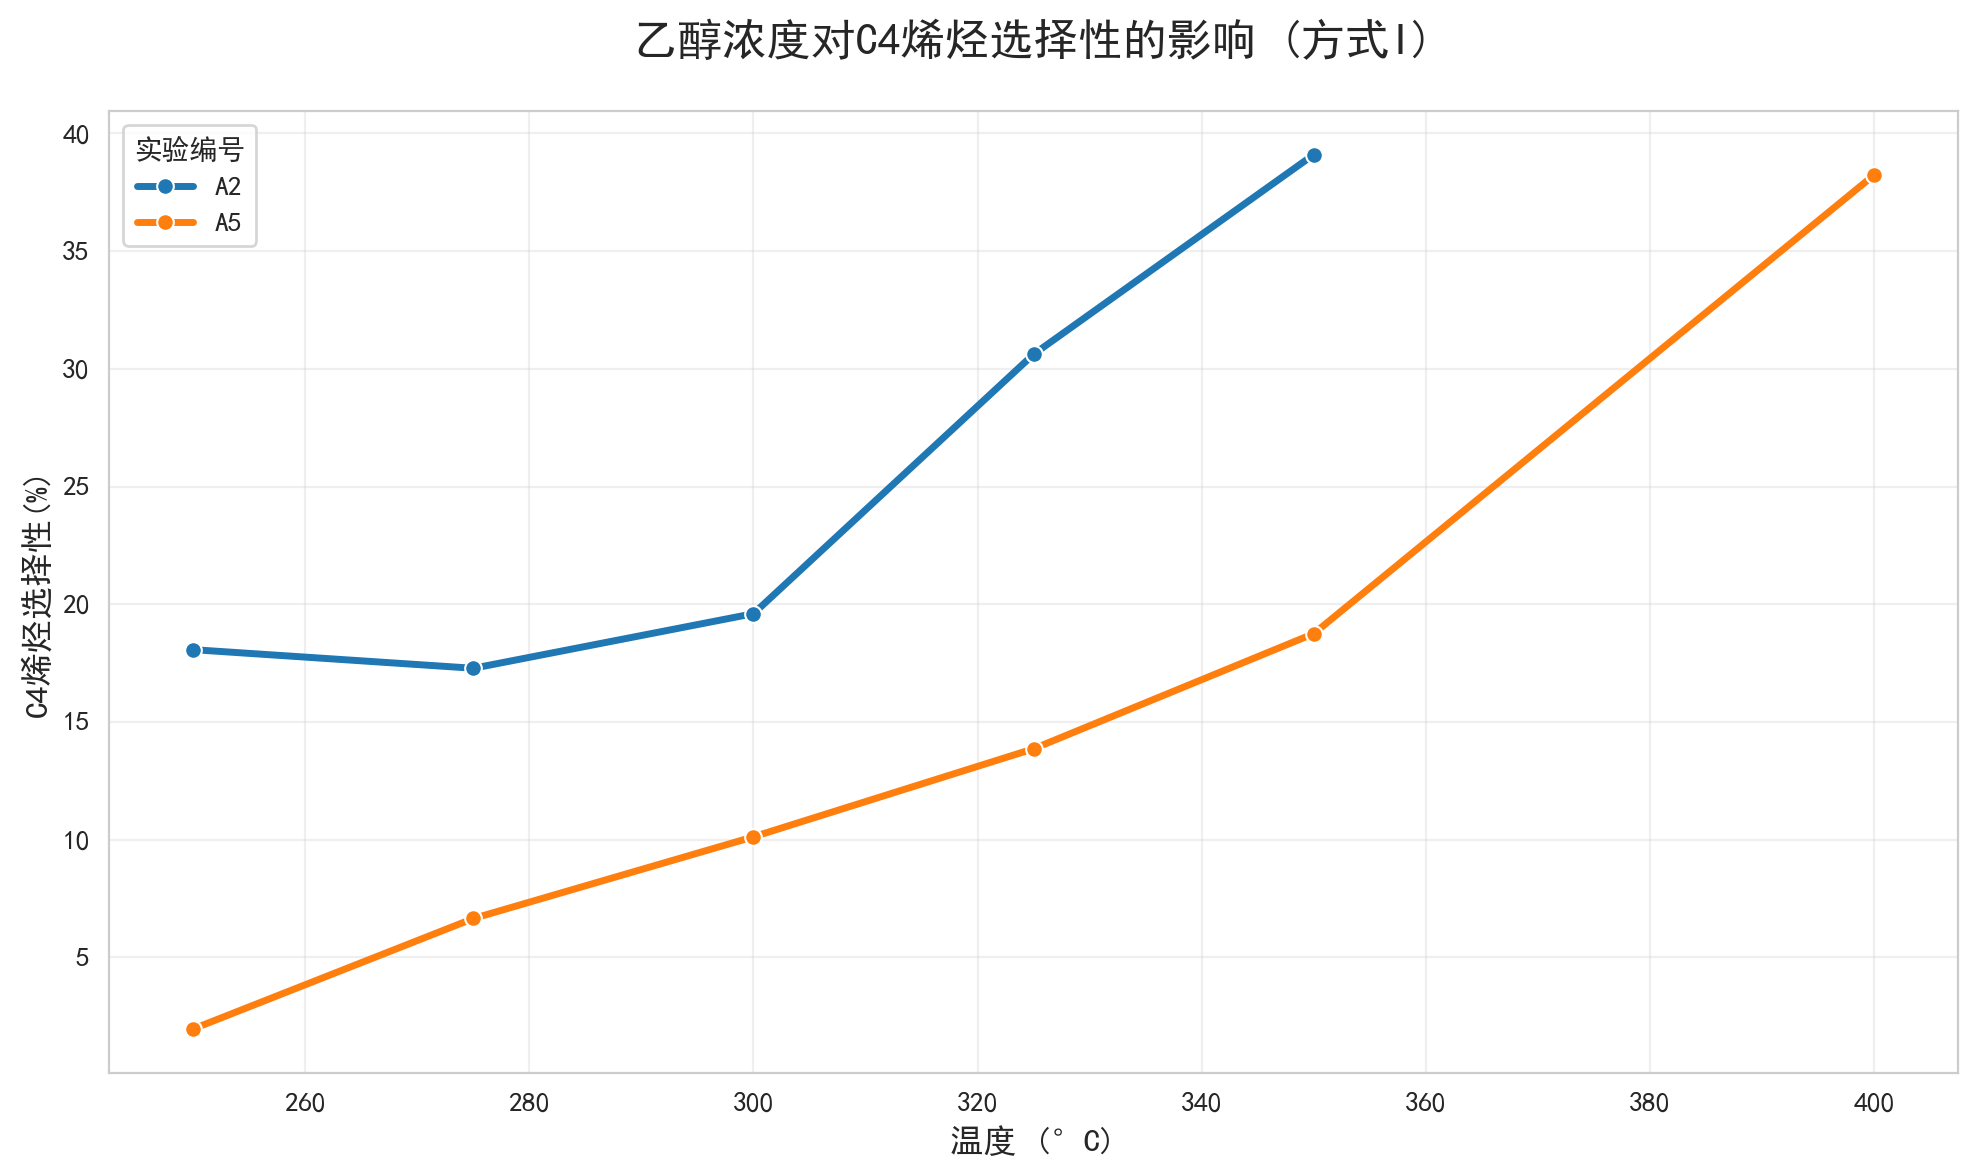
\includegraphics [scale=0.6]{图/2-2-2-1.png}
	\caption{乙醇浓度对C4烯烃选择性的影响 (方式I)} 
	\label{fig:1}
\end{figure}

\begin{figure}[h]%[h]:固定作用
	\centering%置中
	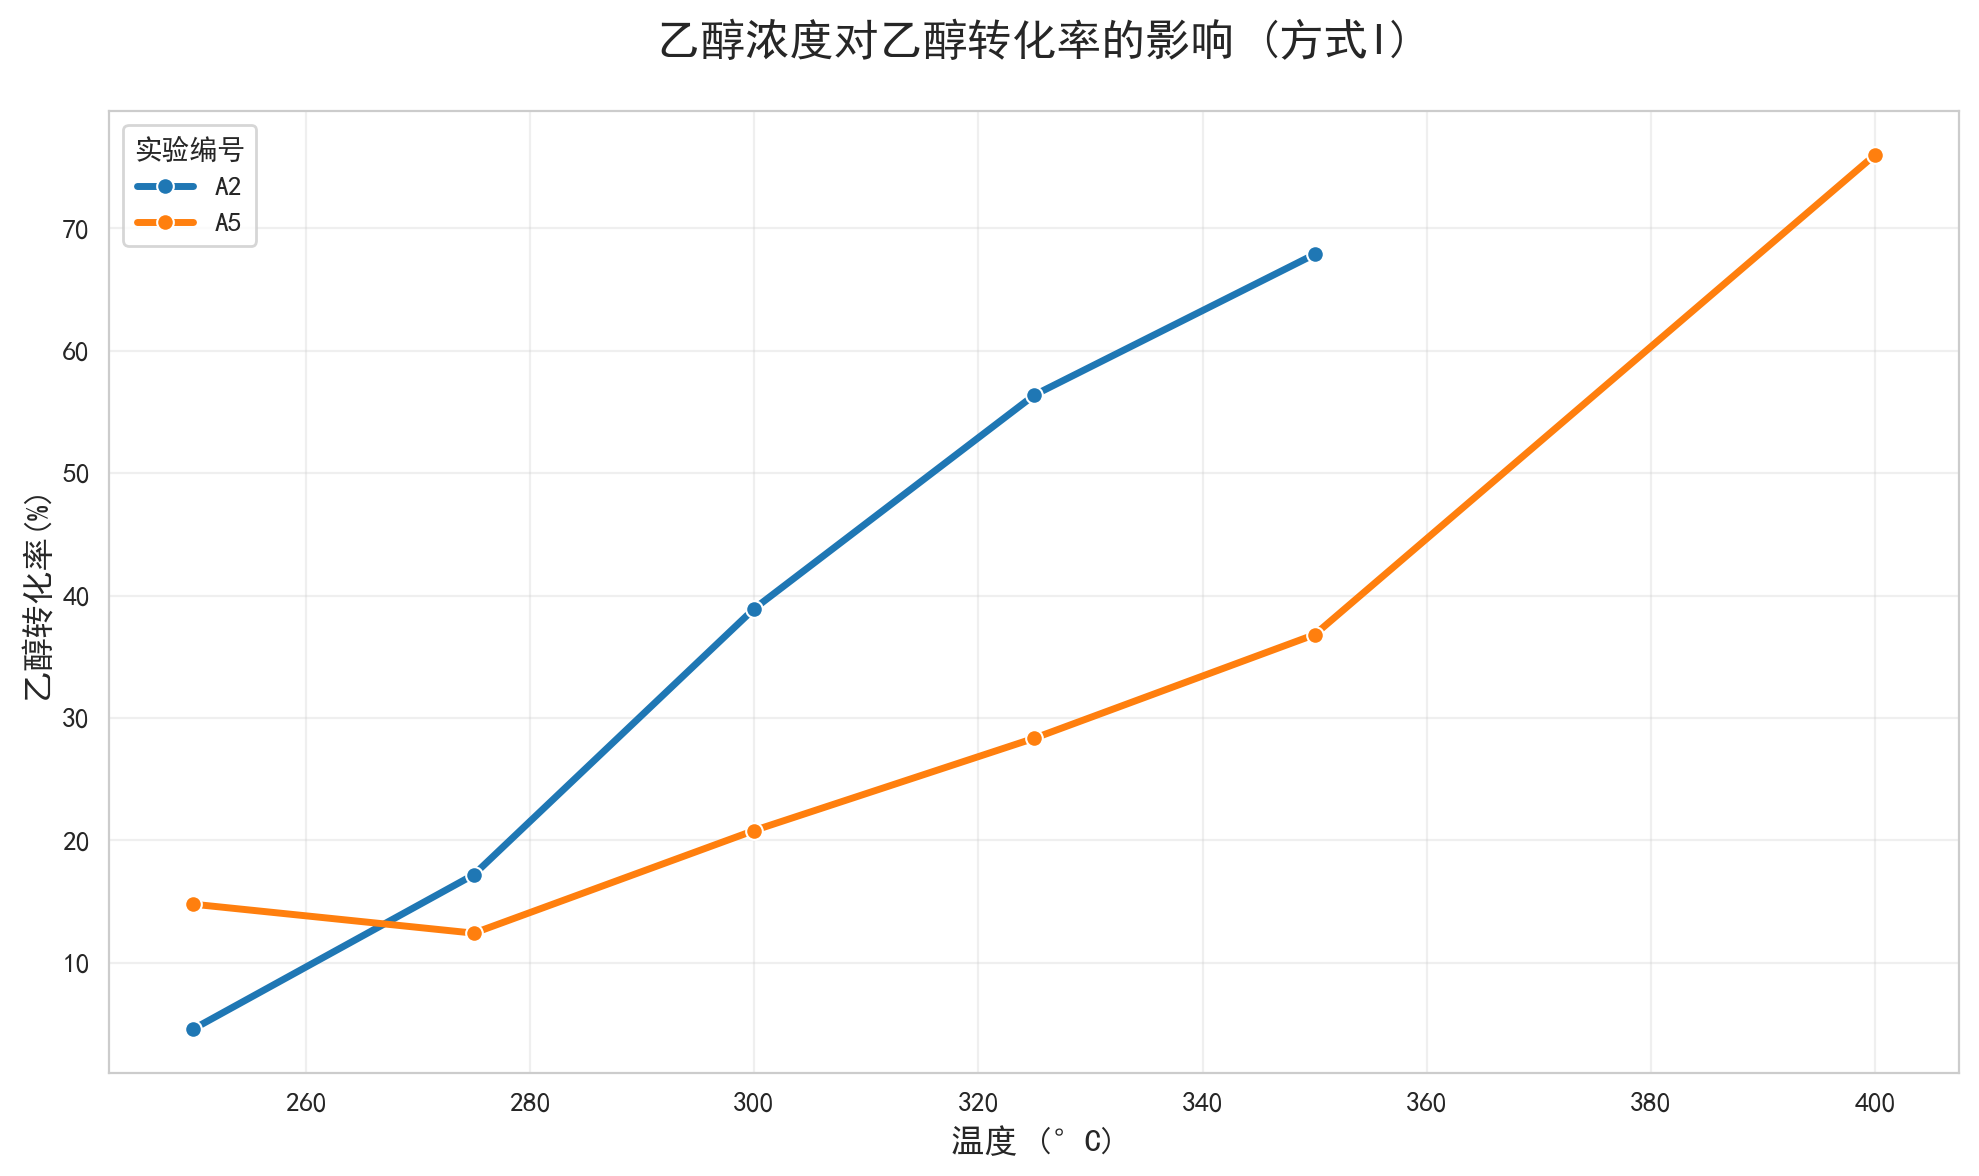
\includegraphics [scale=0.6]{图/2-2-2-2.png}
	\caption{乙醇浓度对乙醇转化率的影响 (方式I)} 
	\label{fig:1}
\end{figure}

\begin{figure}[h]%[h]:固定作用
	\centering%置中
	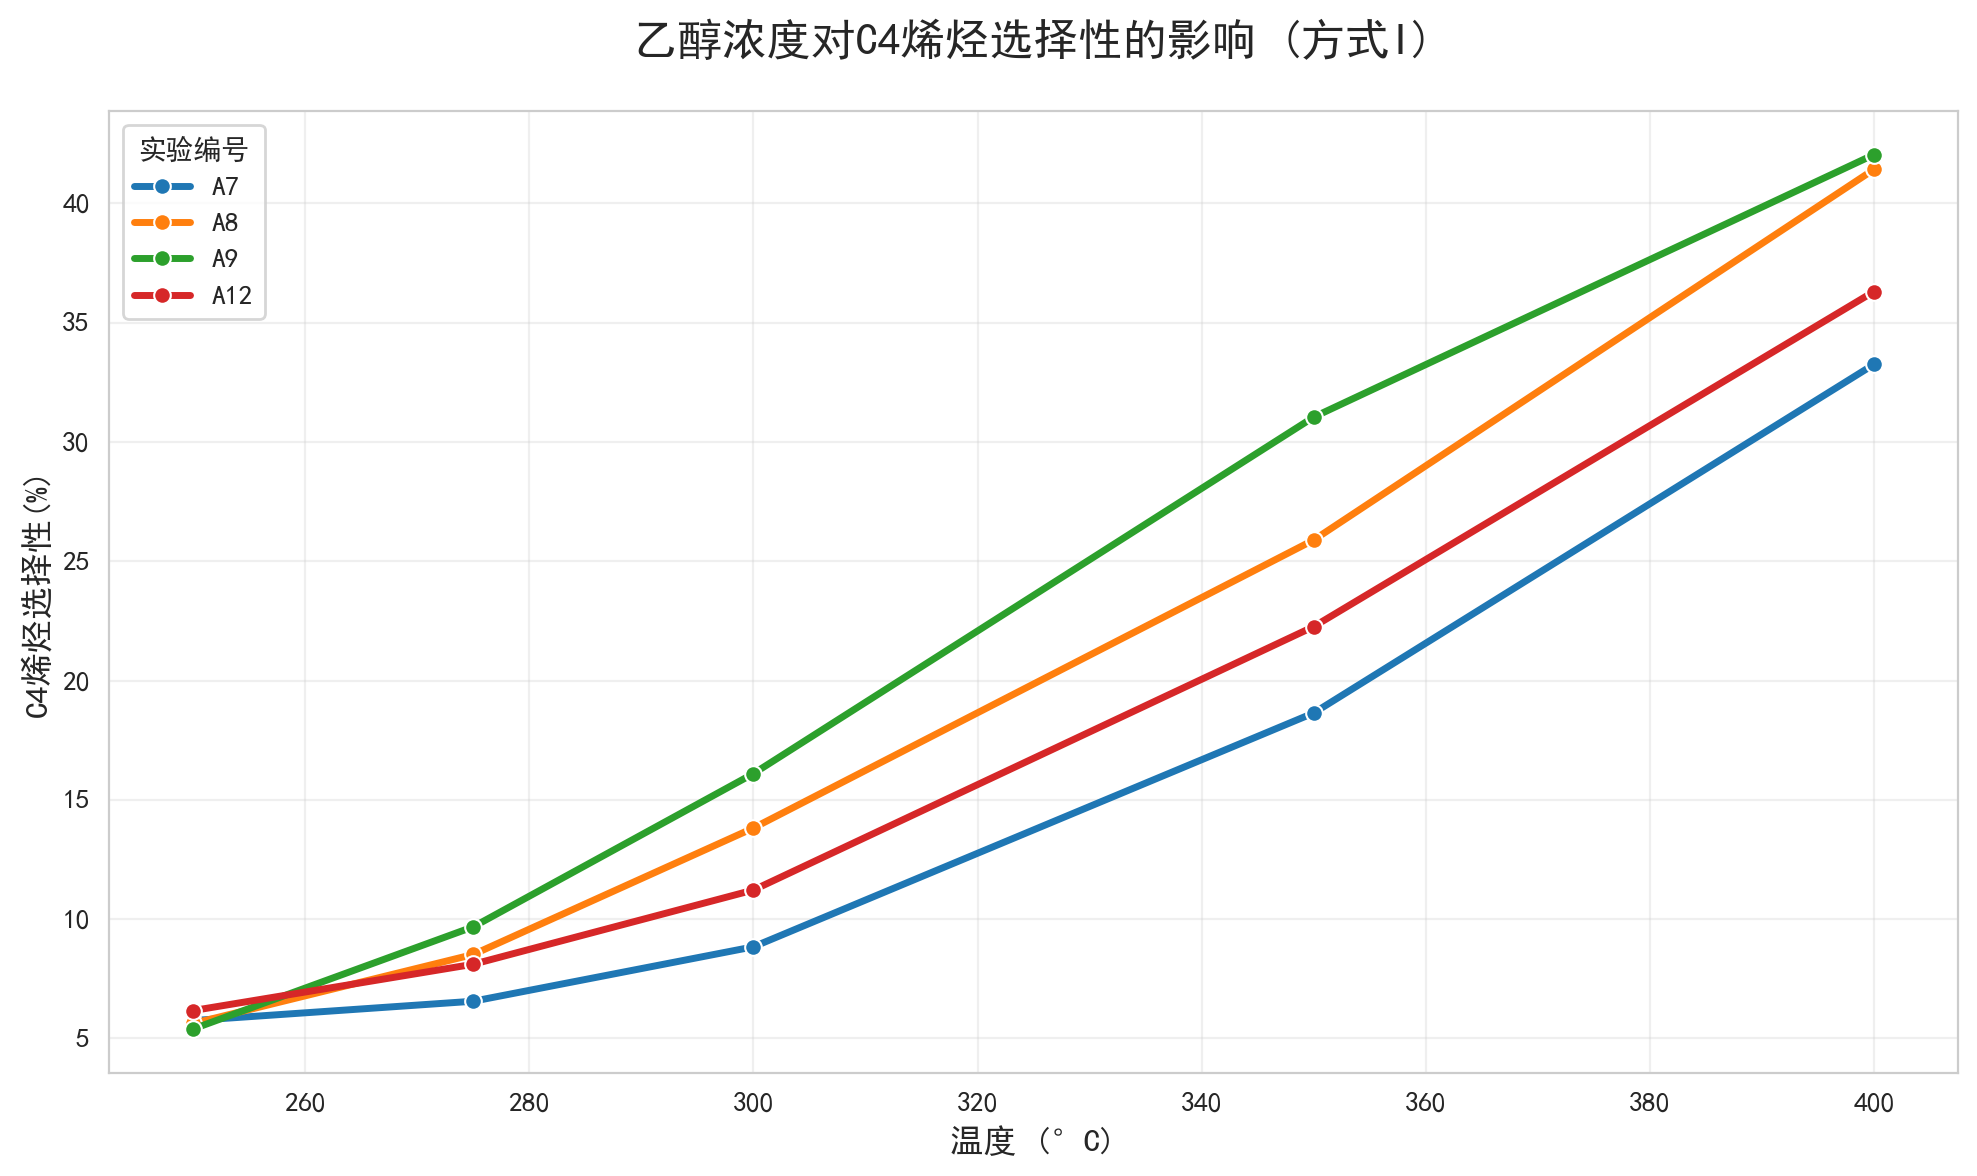
\includegraphics [scale=0.6]{图/2-2-3-1.png}
	\caption{乙醇浓度对C4烯烃选择性的影响 (方式I)} 
	\label{fig:1}
\end{figure}

\begin{figure}[h]%[h]:固定作用
	\centering%置中
	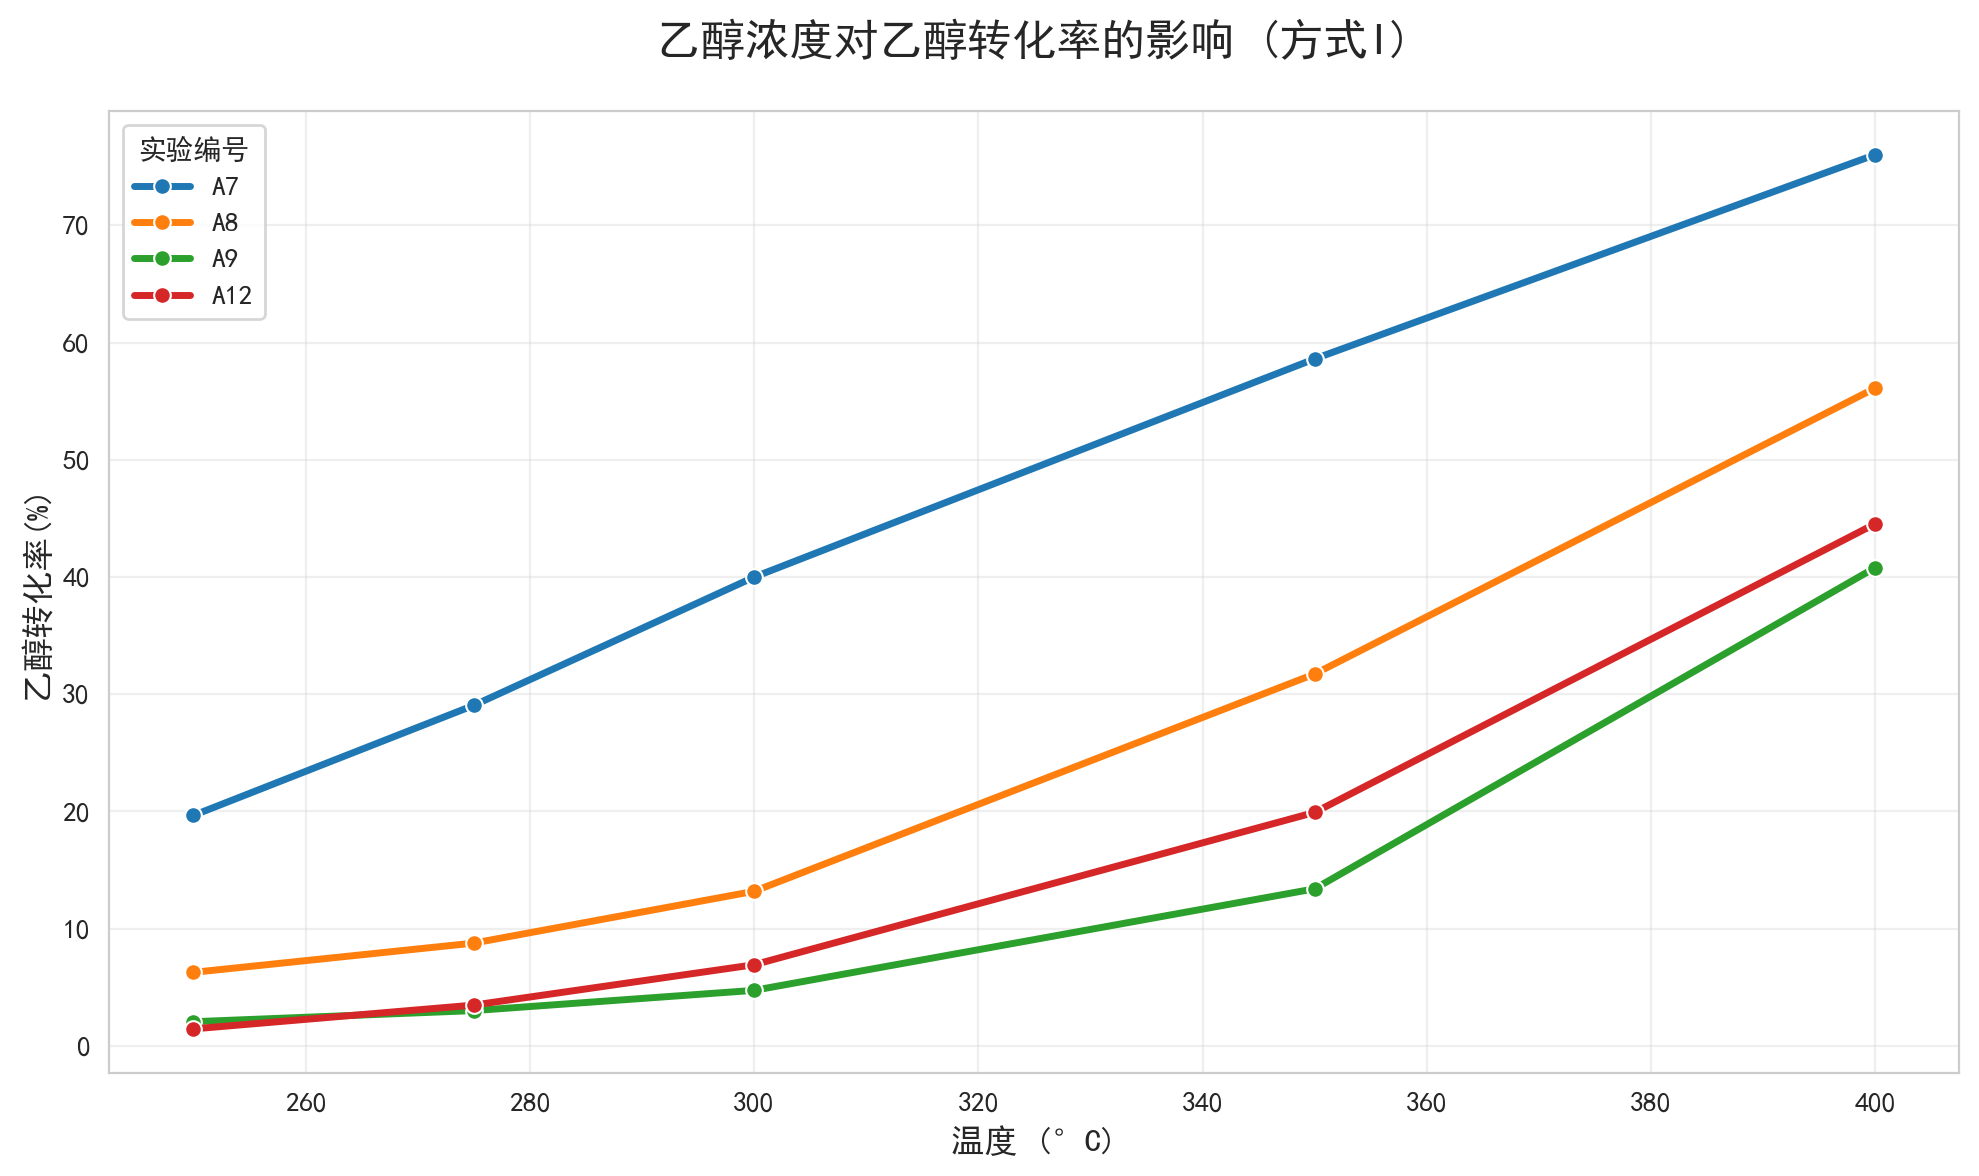
\includegraphics [scale=0.6]{图/2-2-3-2.png}
	\caption{乙醇浓度对乙醇转化率的影响 (方式I)} 
	\label{fig:1}
\end{figure}

\begin{figure}[h]%[h]:固定作用
	\centering%置中
	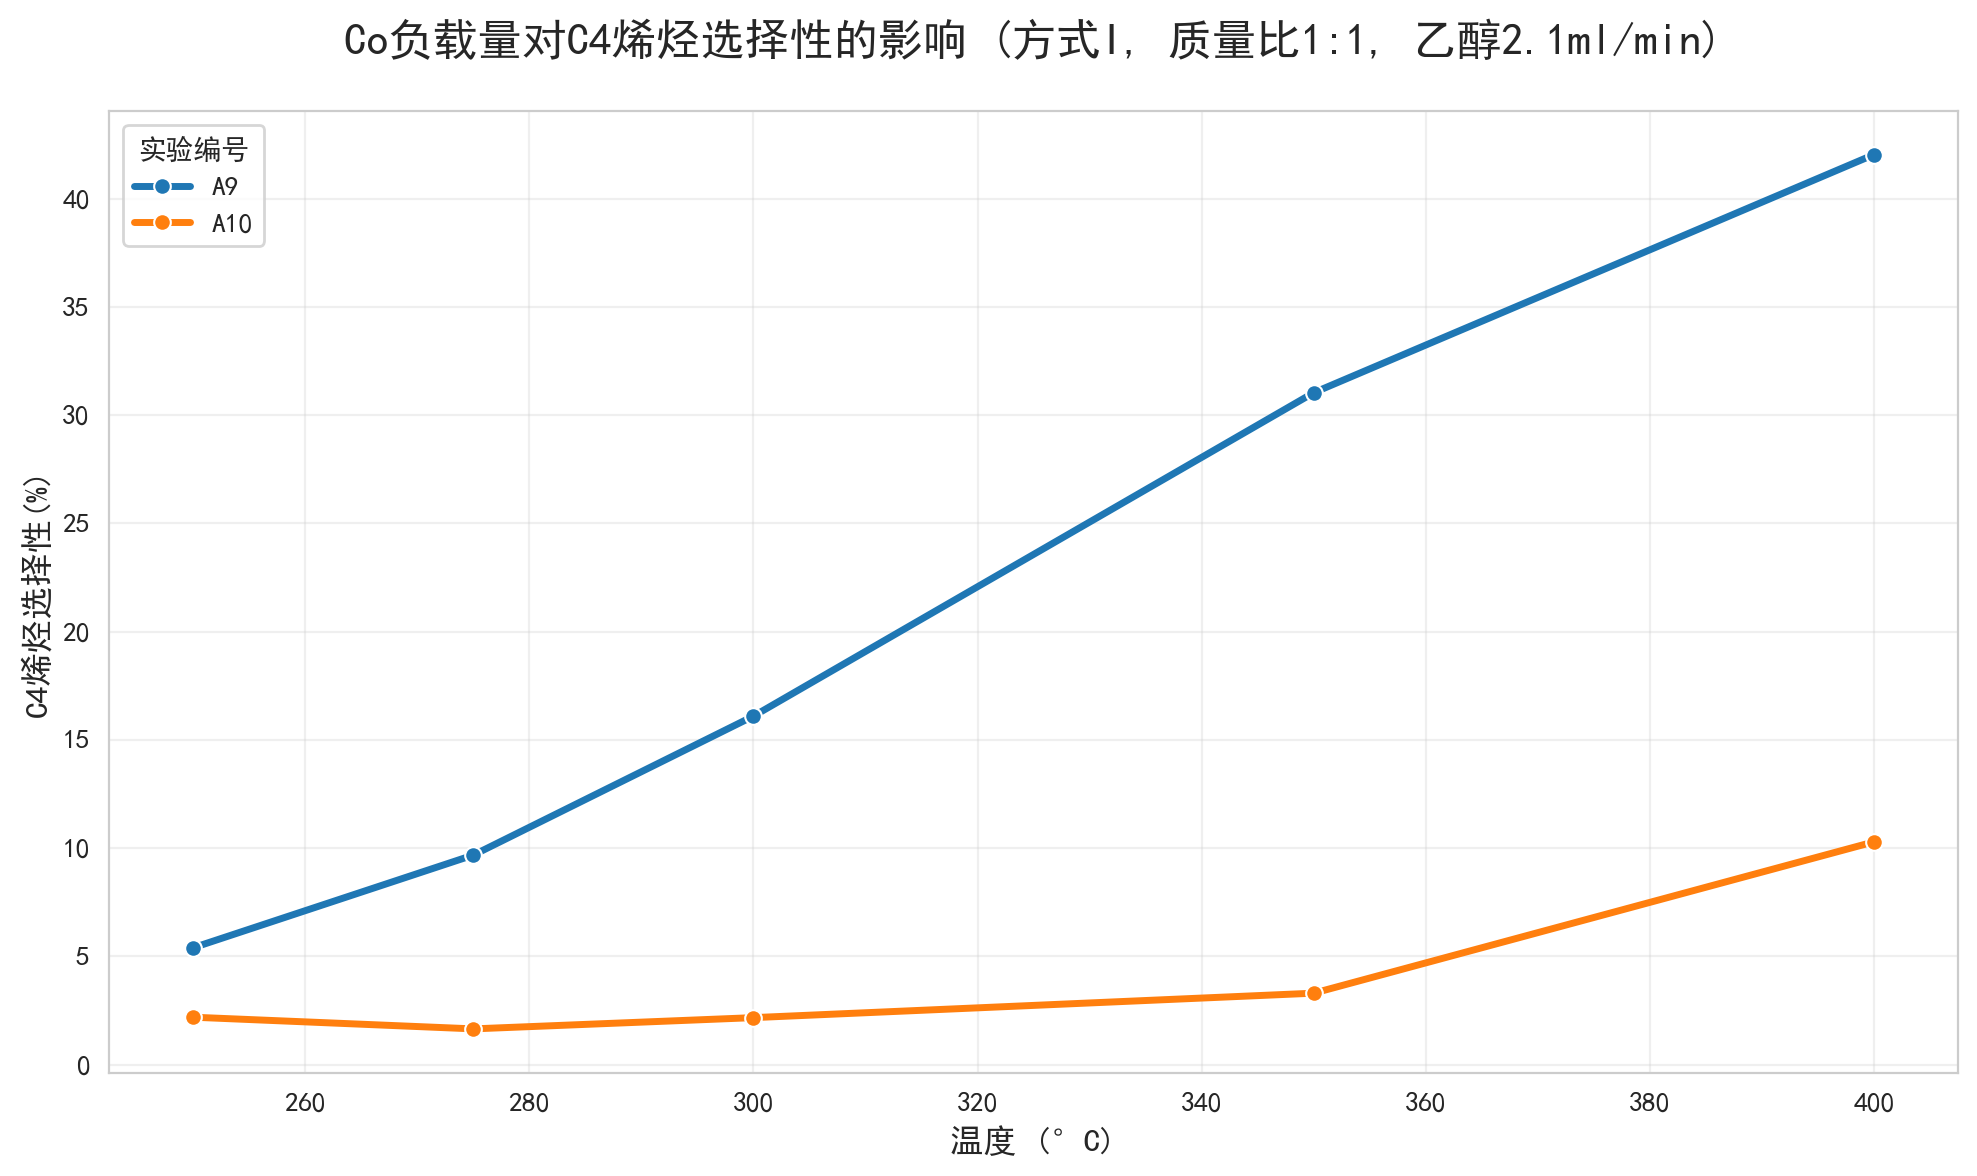
\includegraphics [scale=0.6]{图/2-3-2-1.png}
	\caption{乙醇浓度对C4烯烃选择性的影响 (方式I)} 
	\label{fig:1}
\end{figure}

\begin{figure}[h]%[h]:固定作用
	\centering%置中
	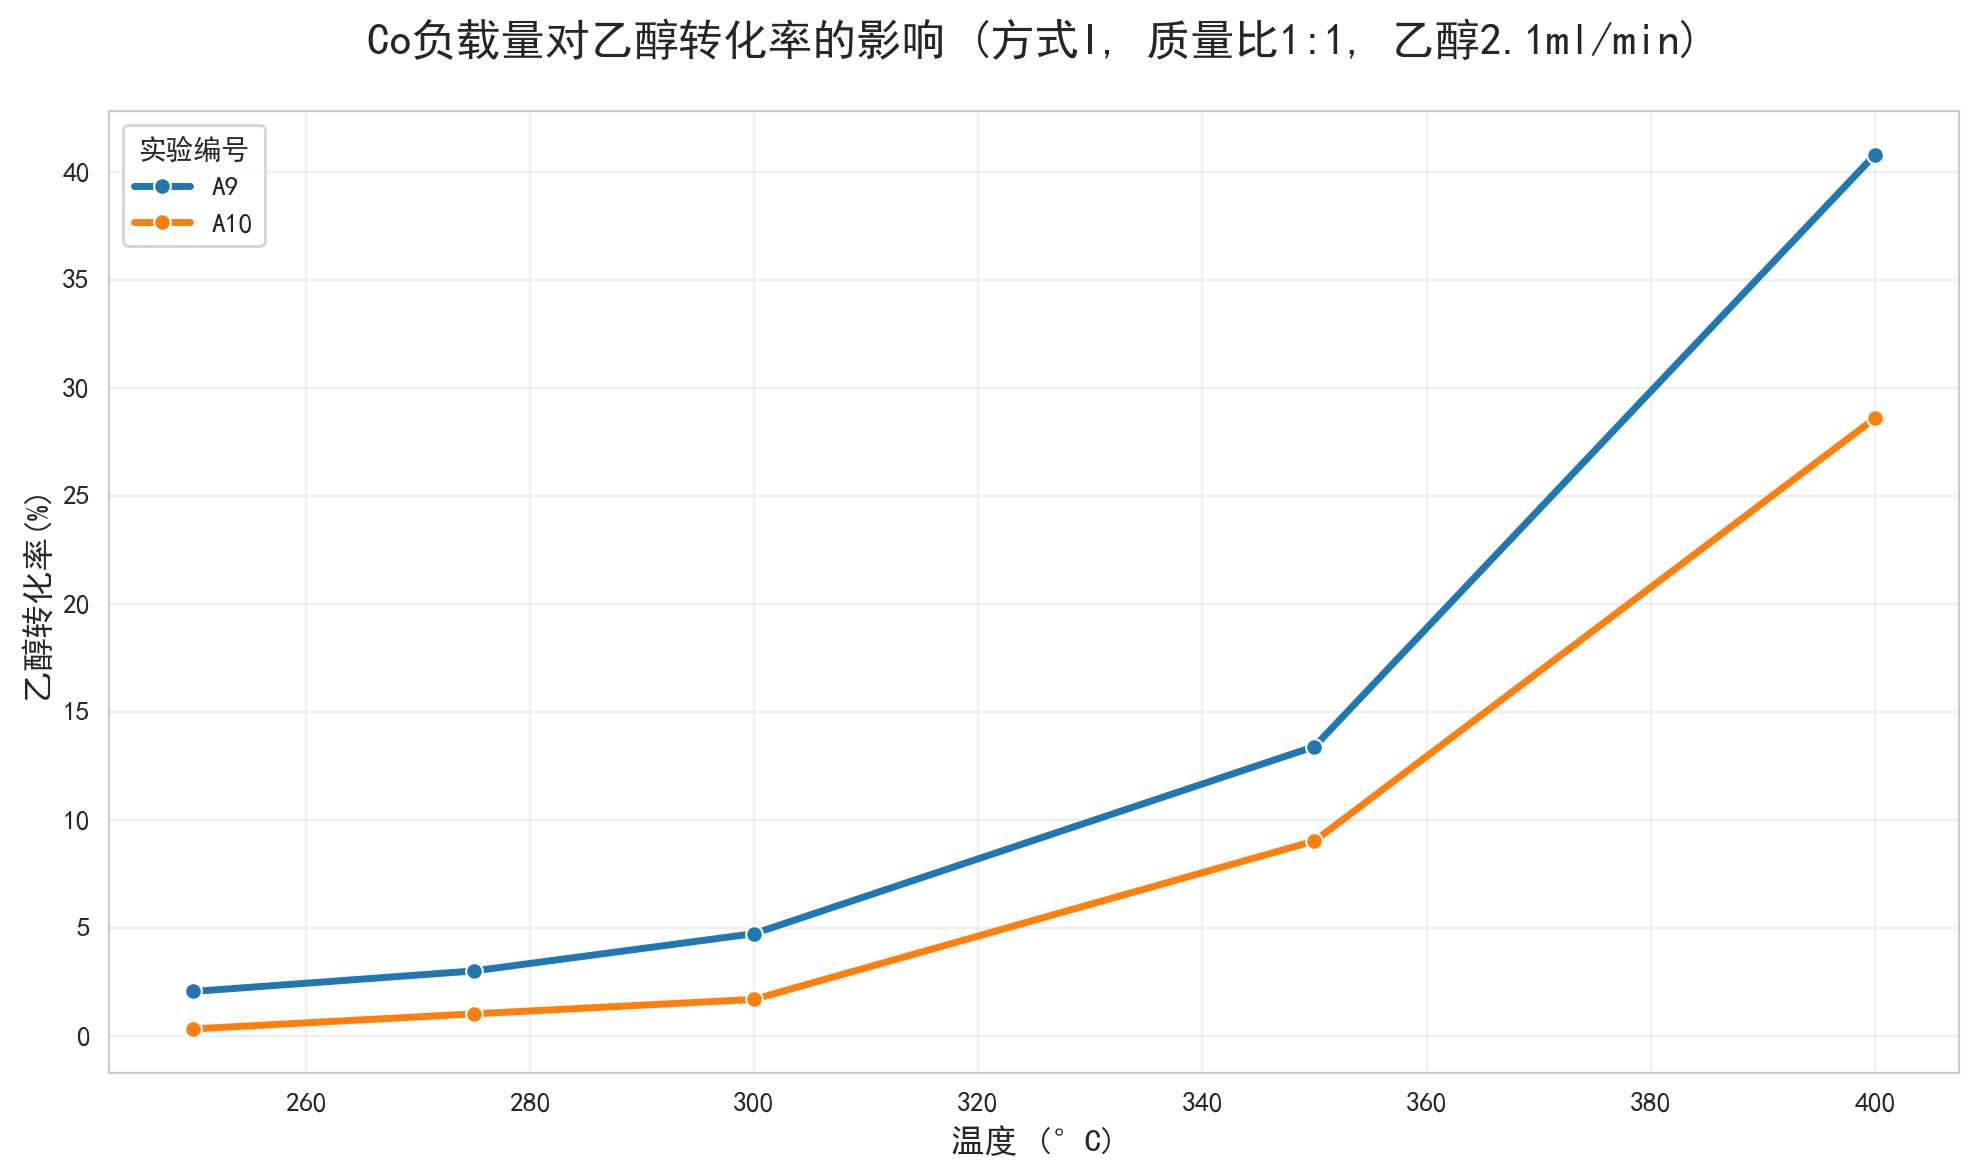
\includegraphics [scale=0.6]{图/2-3-2-2.png}
	\caption{乙醇浓度对乙醇转化率的影响 (方式I)} 
	\label{fig:1}
\end{figure}

\begin{figure}[h]%[h]:固定作用
	\centering%置中
	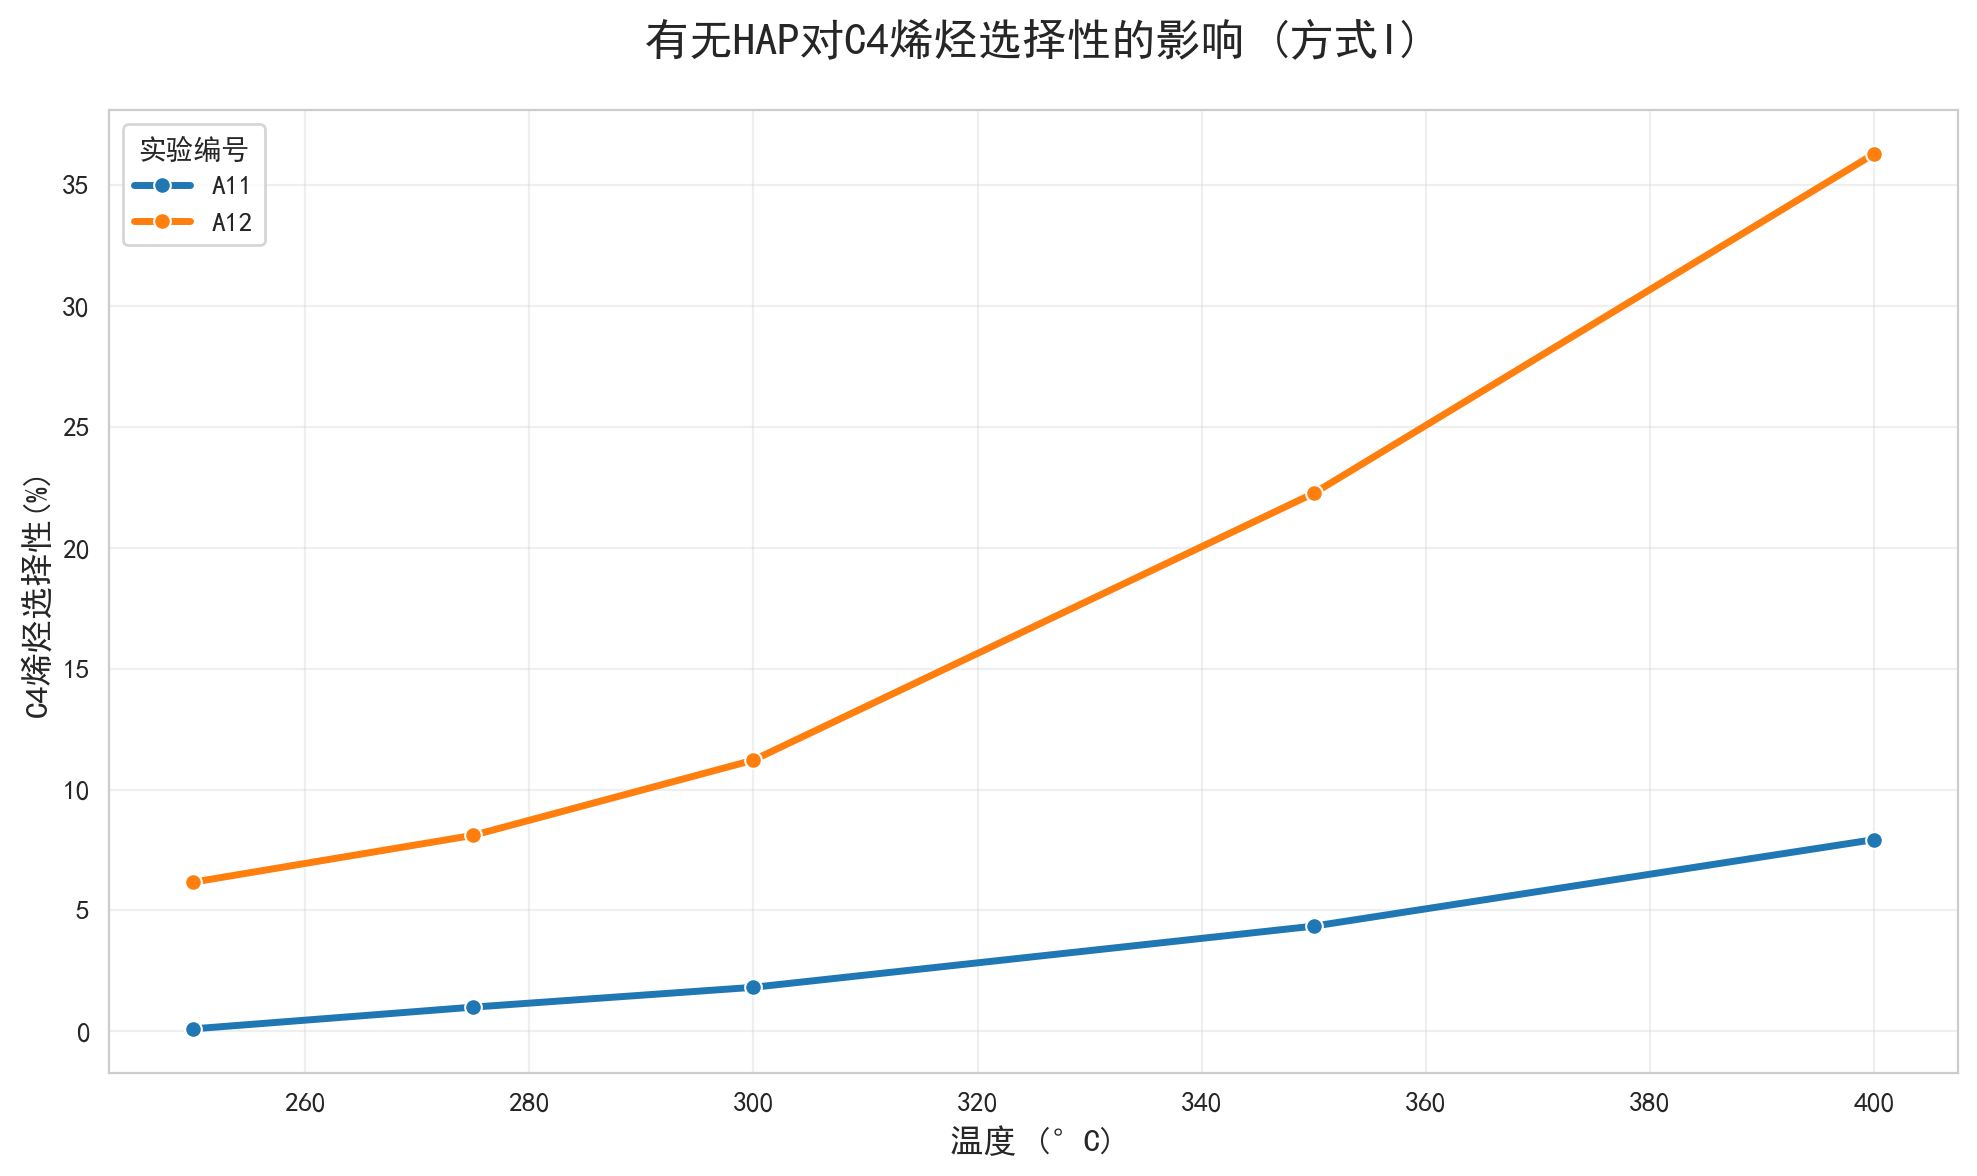
\includegraphics [scale=0.6]{图/2-4-1-1.png}
	\caption{有无HAP对C4烯烃选择性的影响 (方式I)} 
	\label{fig:1}
\end{figure}

\begin{figure}[h]%[h]:固定作用
	\centering%置中
	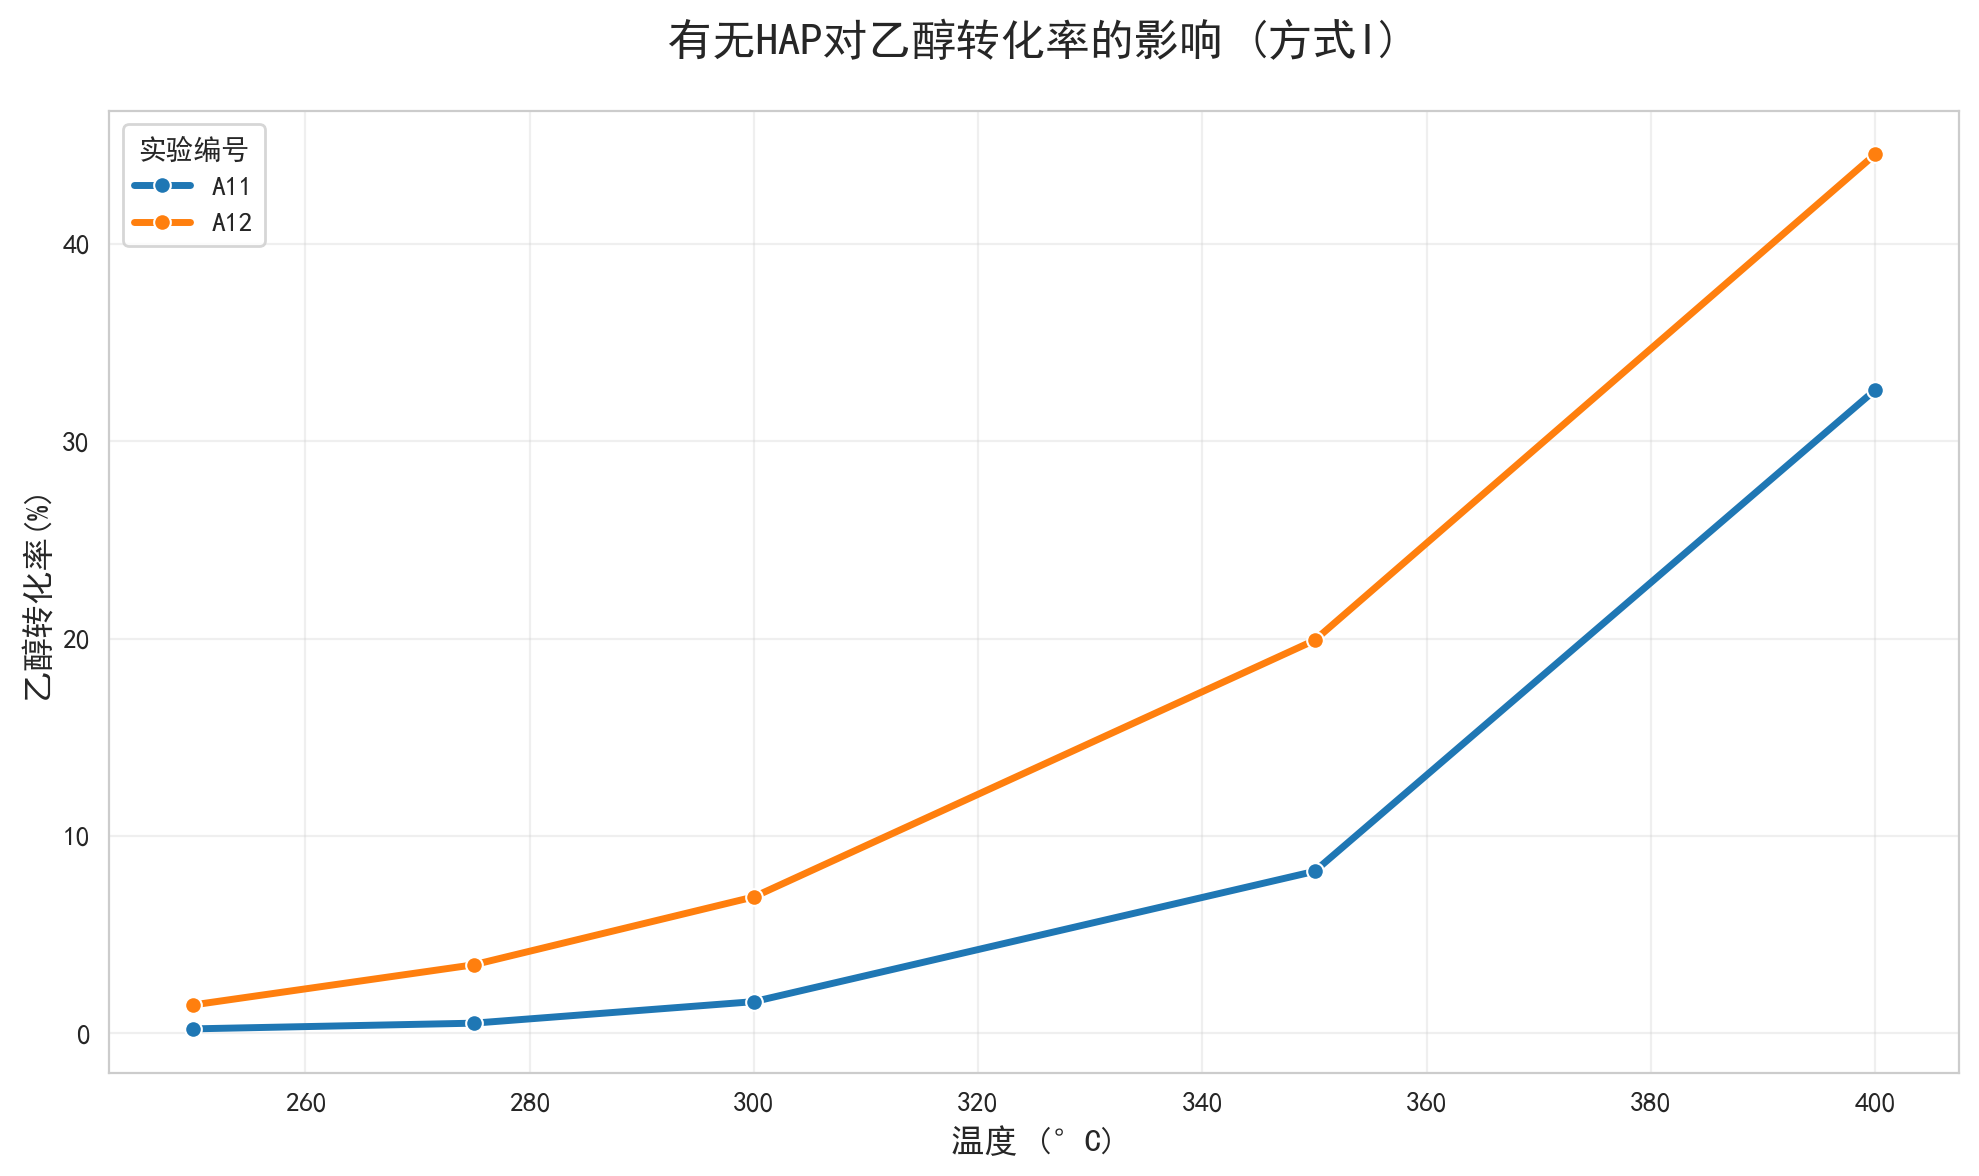
\includegraphics [scale=0.6]{图/2-4-1-2.png}
	\caption{有无HAP对乙醇转化率的影响 (方式I)} 
	\label{fig:1}
\end{figure}

\begin{figure}[h]%[h]:固定作用
	\centering%置中
	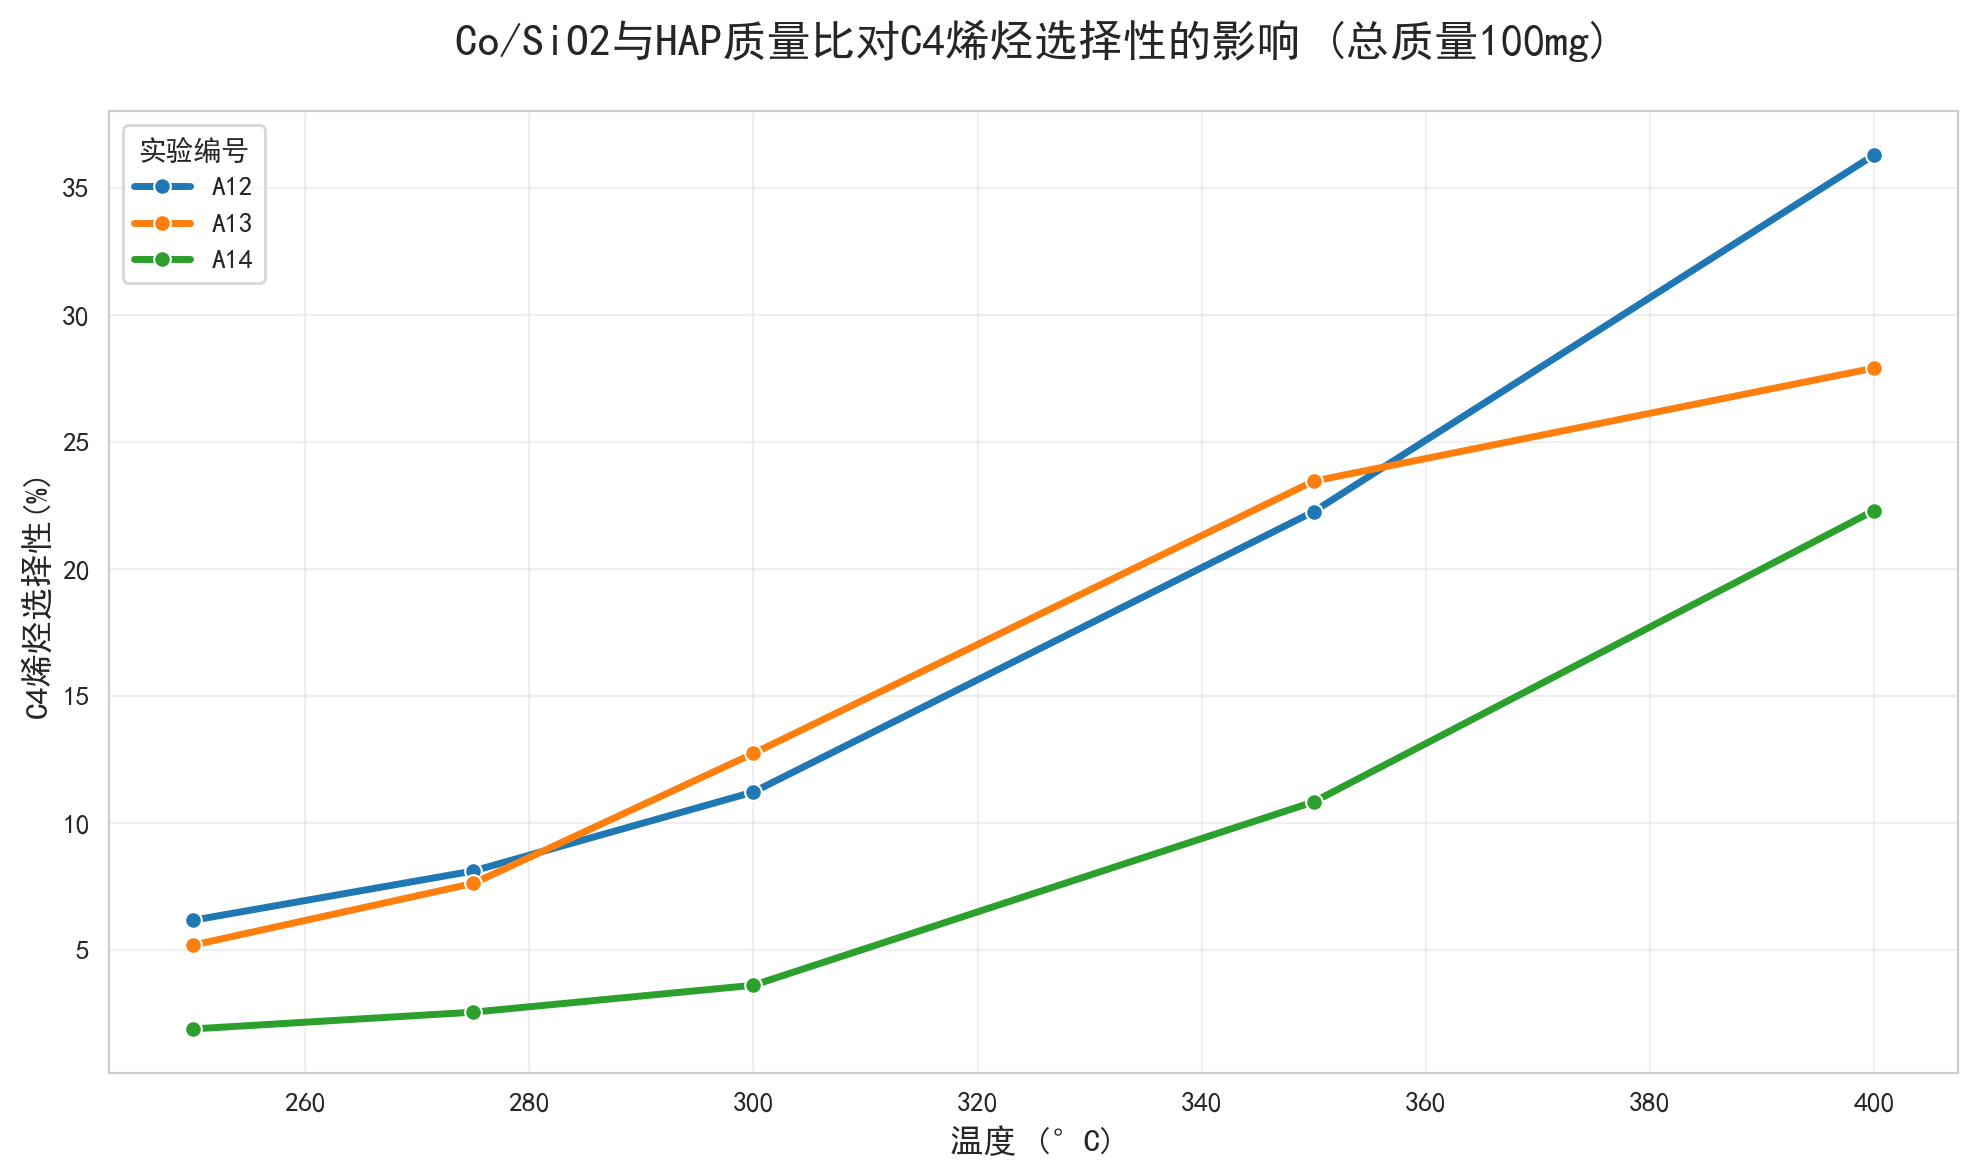
\includegraphics [scale=0.6]{图/2-5-1-1.png}
	\caption{Co/SiO2与HAP质量比对C4烯烃选择性的影响 (总质量100mg)} 
	\label{fig:1}
\end{figure}

\begin{figure}[h]%[h]:固定作用
	\centering%置中
	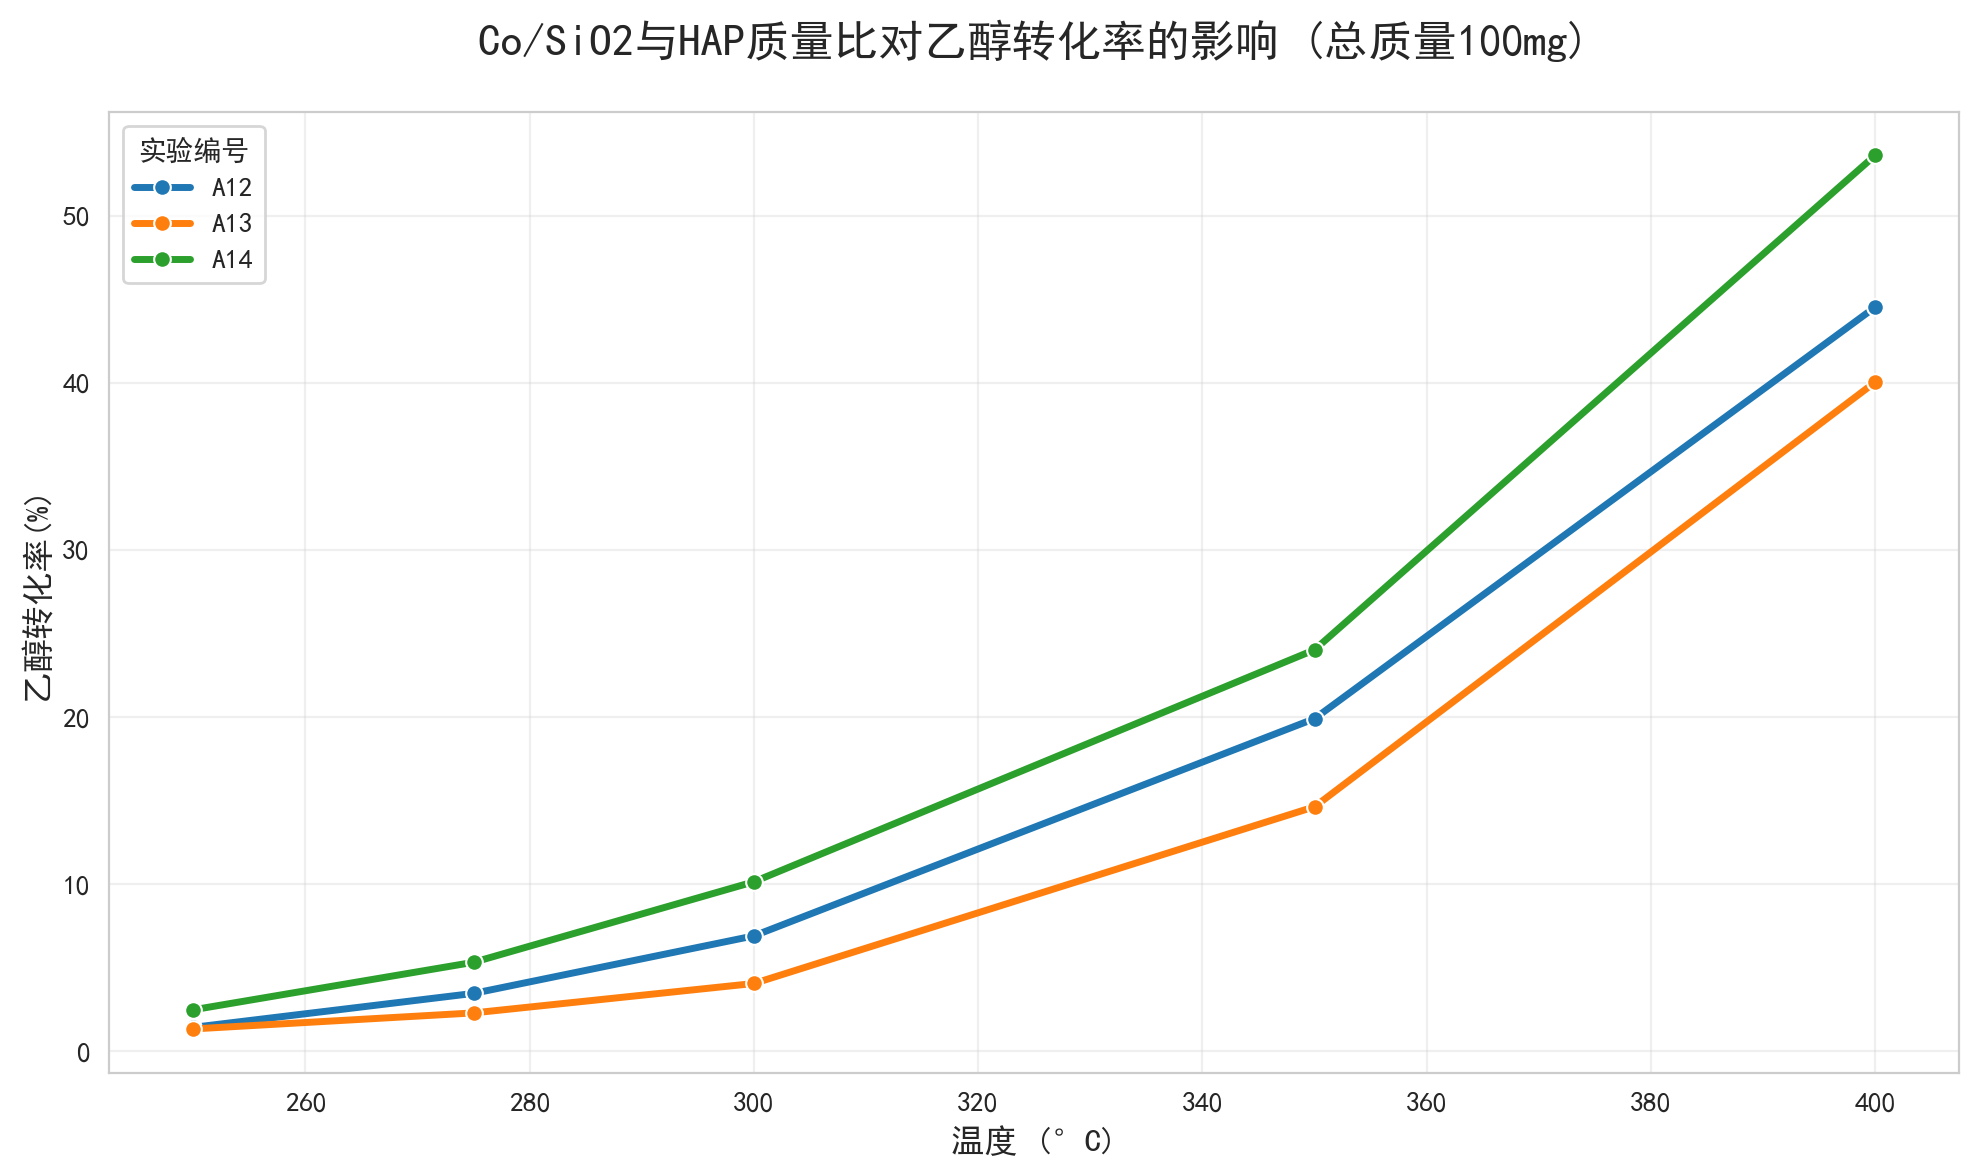
\includegraphics [scale=0.6]{图/2-5-1-2.png}
	\caption{Co/SiO2与HAP质量比对乙醇转化率的影响 (总质量100mg)} 
	\label{fig:1}
\end{figure}

\begin{figure}[h]%[h]:固定作用
	\centering%置中
	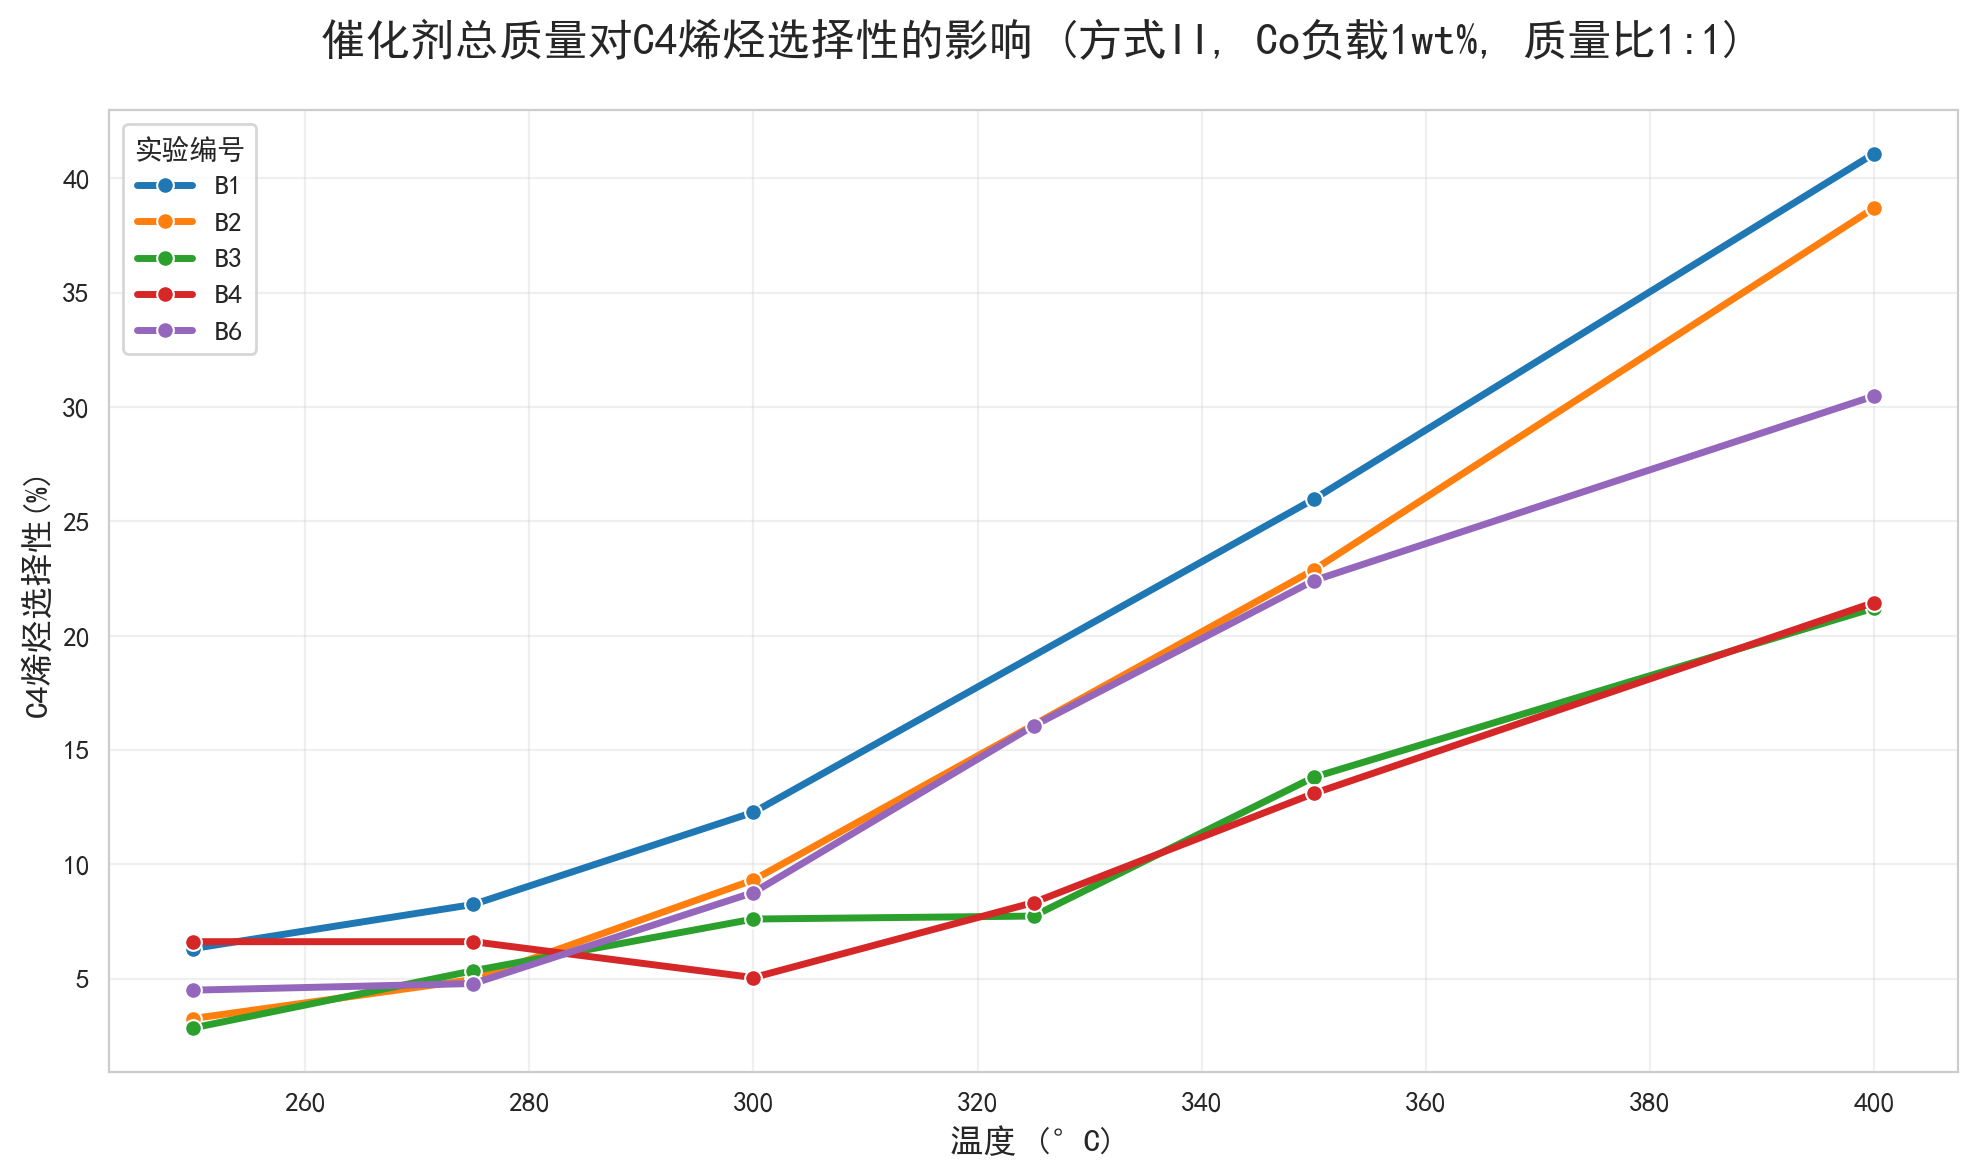
\includegraphics [scale=0.6]{图/2-6-1-1.png}
	\caption{催化剂总质量对C4烯烃选择性的影响 (方式II, Co负载1wt\%, 质量比1:1)} 
	\label{fig:1}
\end{figure}

\begin{figure}[h]%[h]:固定作用
	\centering%置中
	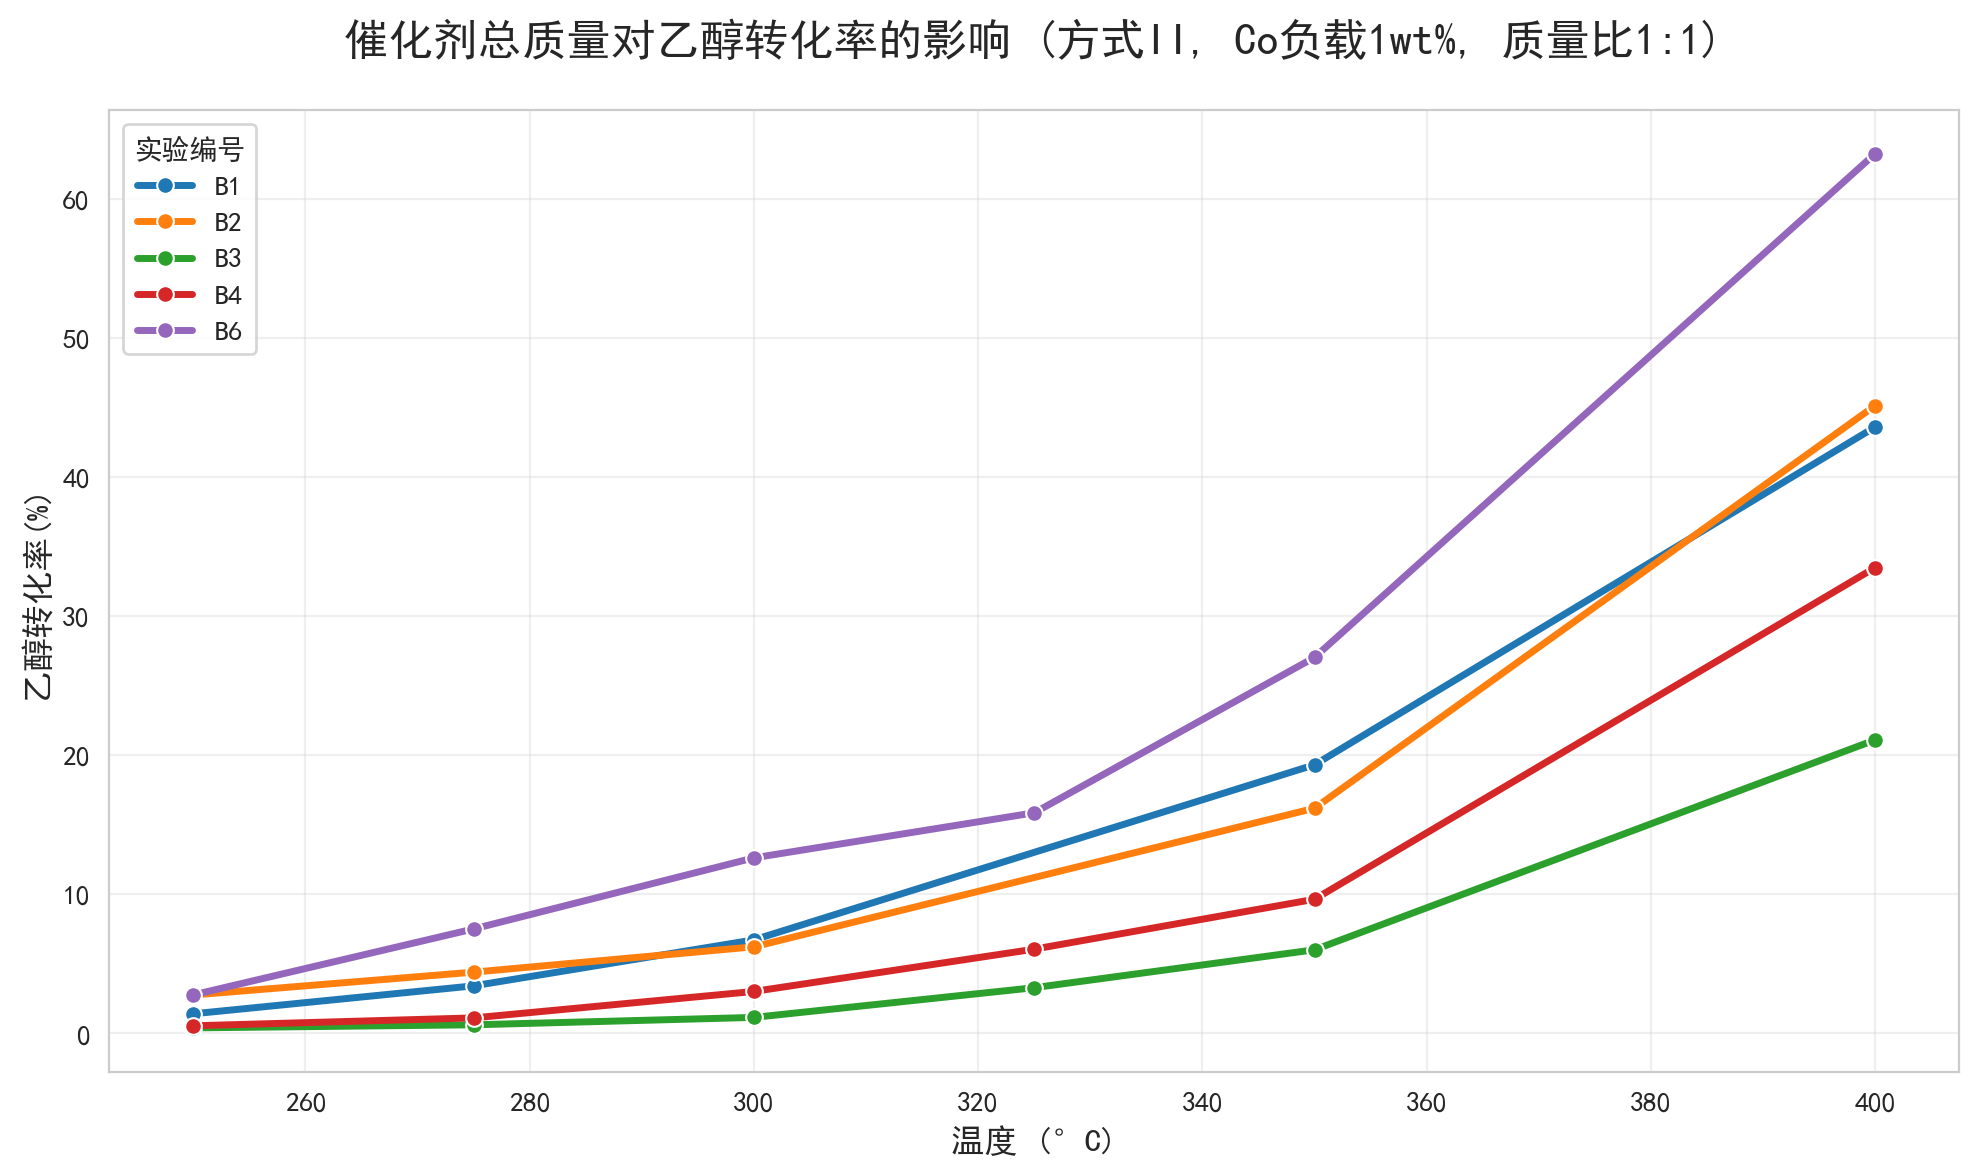
\includegraphics [scale=0.6]{图/2-6-1-2.png}
	\caption{催化剂总质量对乙醇转化率的影响 (方式II, Co负载1wt\%, 质量比1:1)} 
	\label{fig:1}
\end{figure}

\begin{figure}[h]%[h]:固定作用
	\centering%置中
	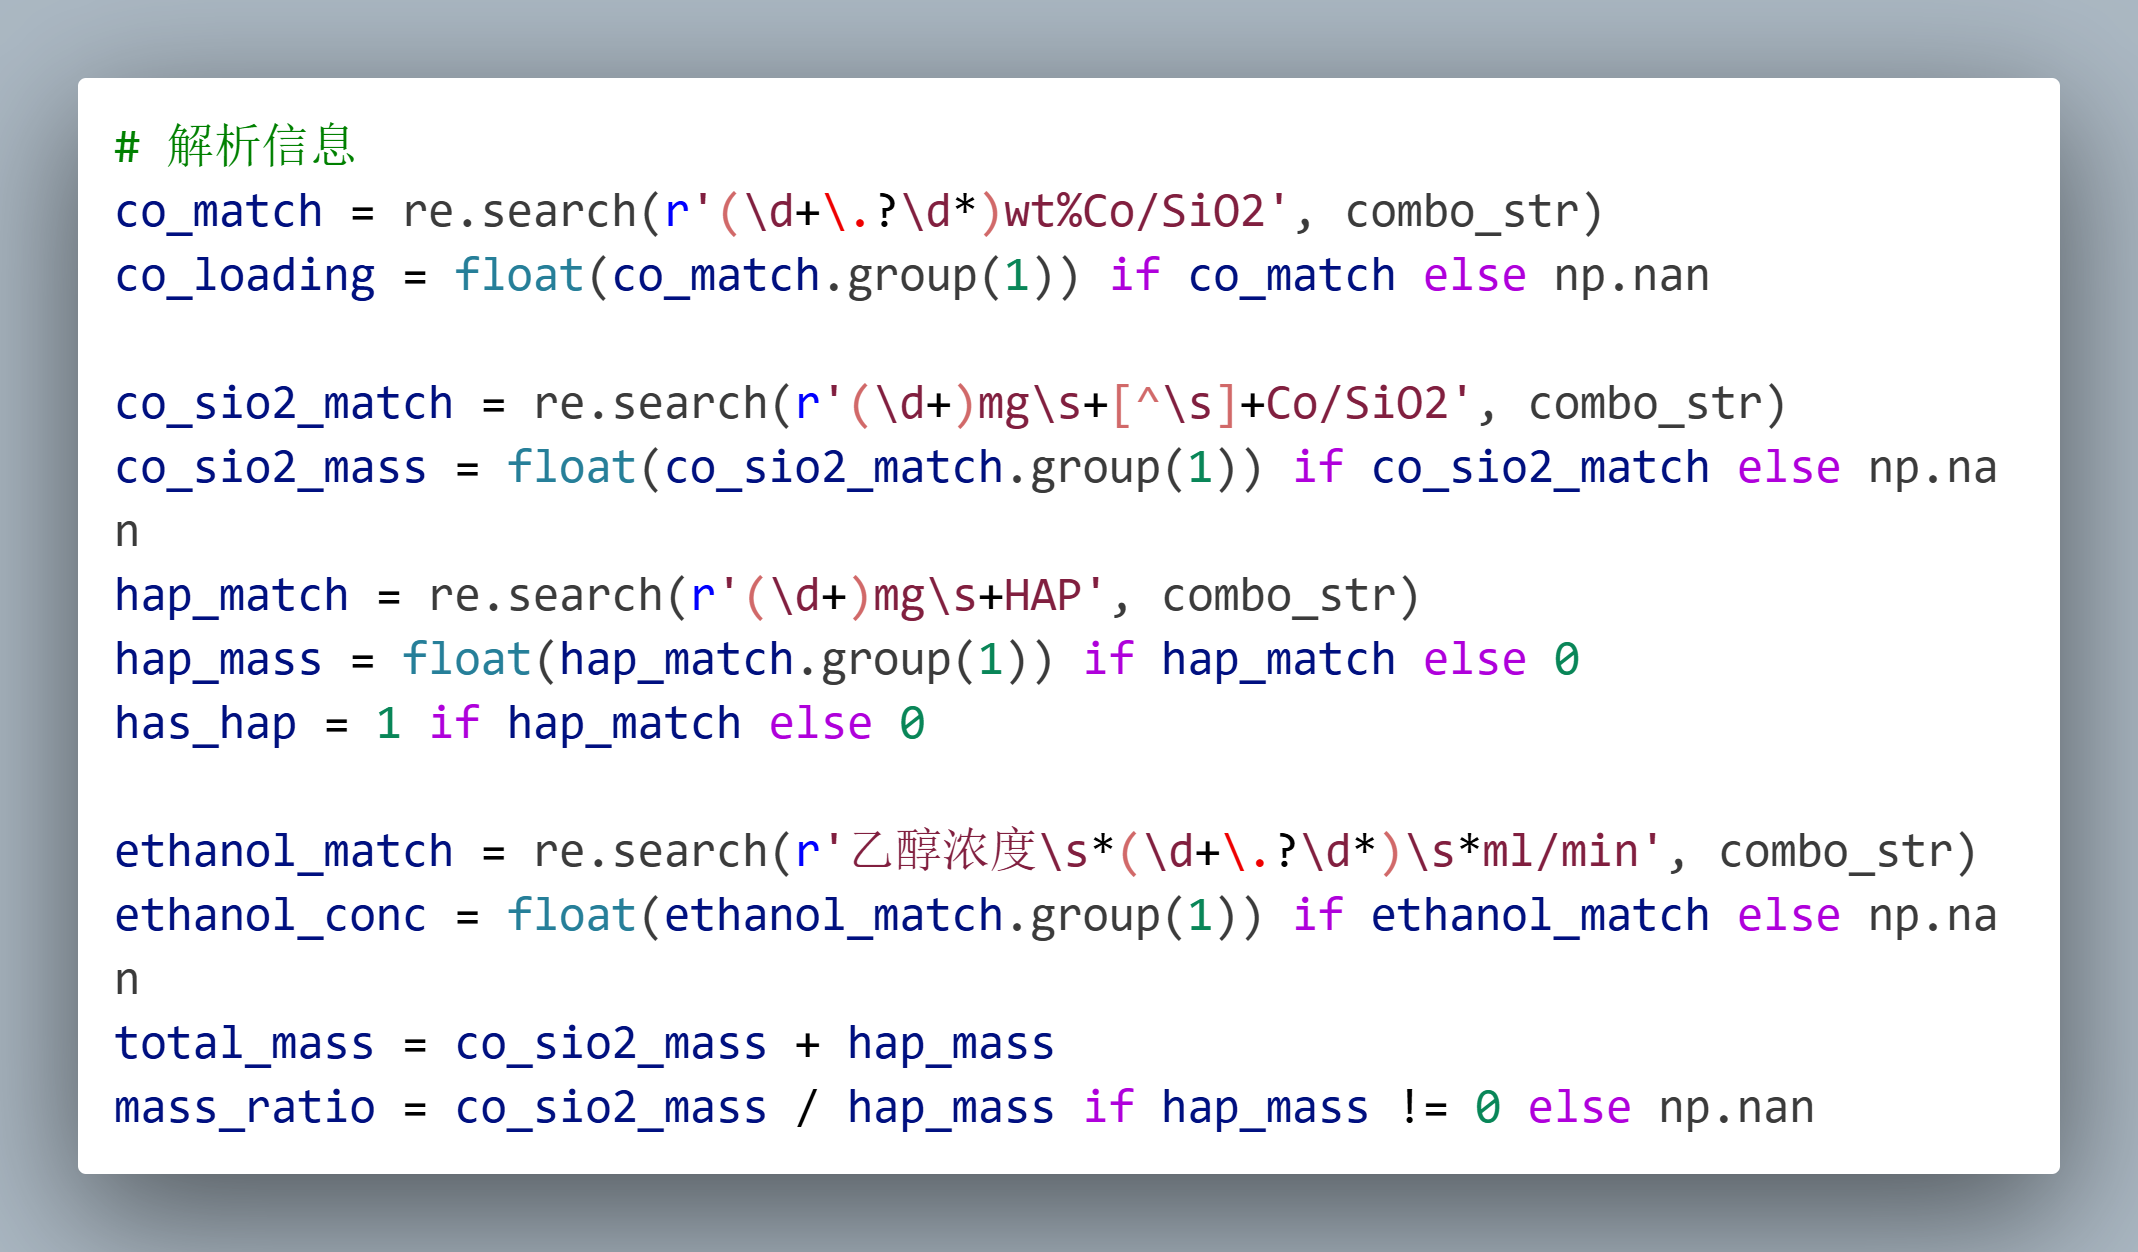
\includegraphics [scale=0.2]{图/code_1.png}
	\caption{Python正则化表达式代码} 
	\label{fig:1}
\end{figure}

\begin{figure}[h]%[h]:固定作用
	\centering%置中
	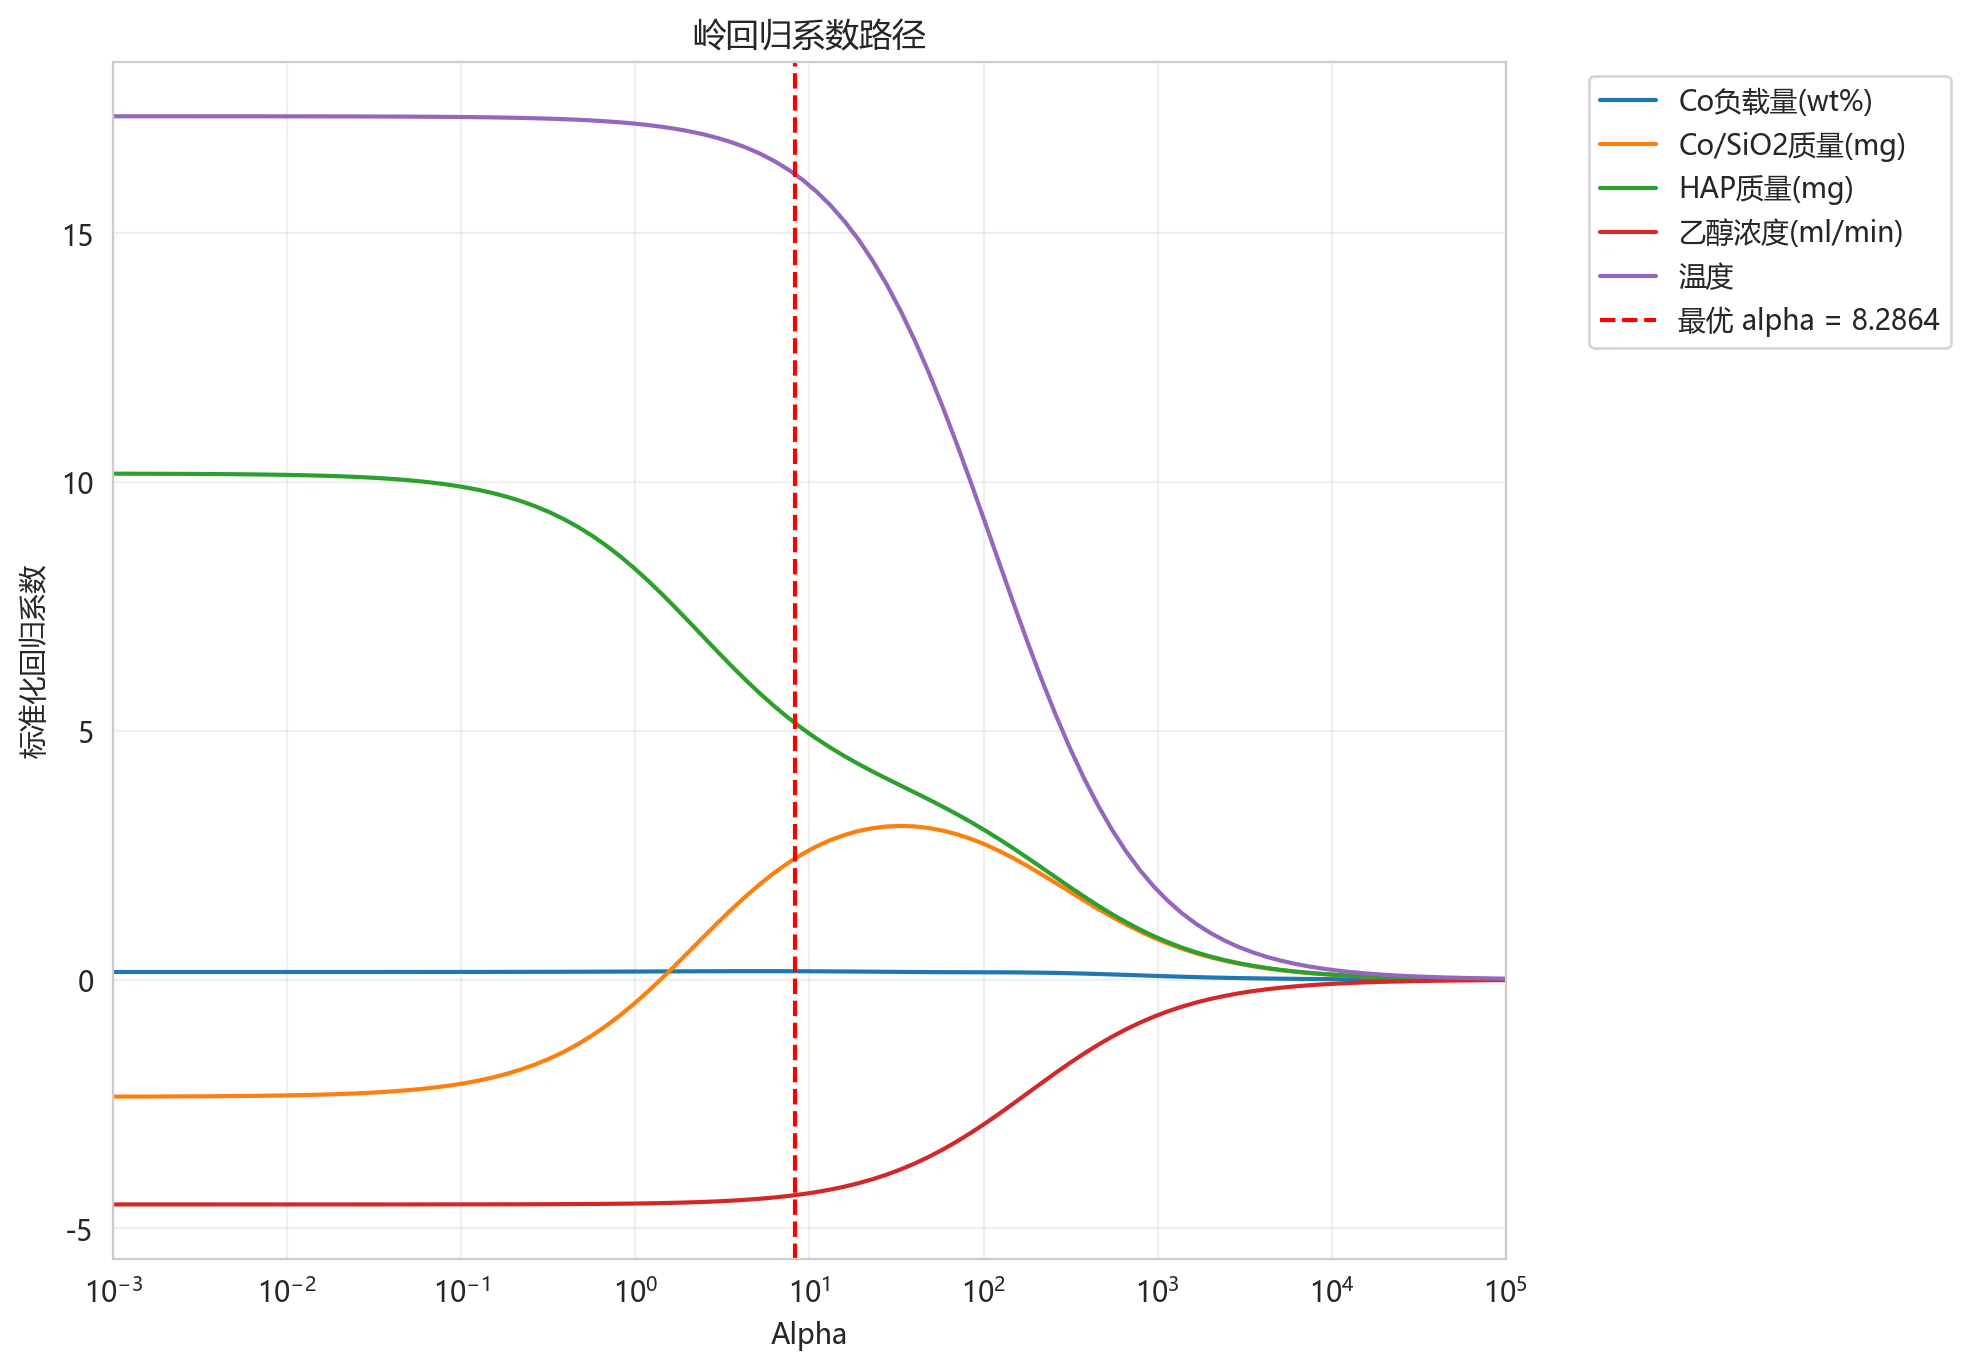
\includegraphics [scale=0.6]{图/ling-yichun.png}
	\caption{乙醇转化率岭回归系数路径} 
	\label{fig:1}
\end{figure}

\begin{table}[!htbp]
	\caption{乙醇转化率模型的标准化回归系数}
	\centering
	\begin{tabular}{l c}
		\hline
		\multicolumn{1}{c}{\textbf{特征名称}} & \textbf{标准化回归系数} \\
		\hline
		Co负载量(wt\%)      & 0.1697 \\
		Co/SiO2质量(mg)     & 2.4395 \\
		HAP质量(mg)         & 5.1538 \\
		乙醇浓度(ml/min)    & -4.3307 \\
		温度 (°C)                & 16.1869 \\
		\hline
		\label{tab:ridge_coefficients}
	\end{tabular}
\end{table}

\begin{figure}[h]%[h]:固定作用
	\centering%置中
	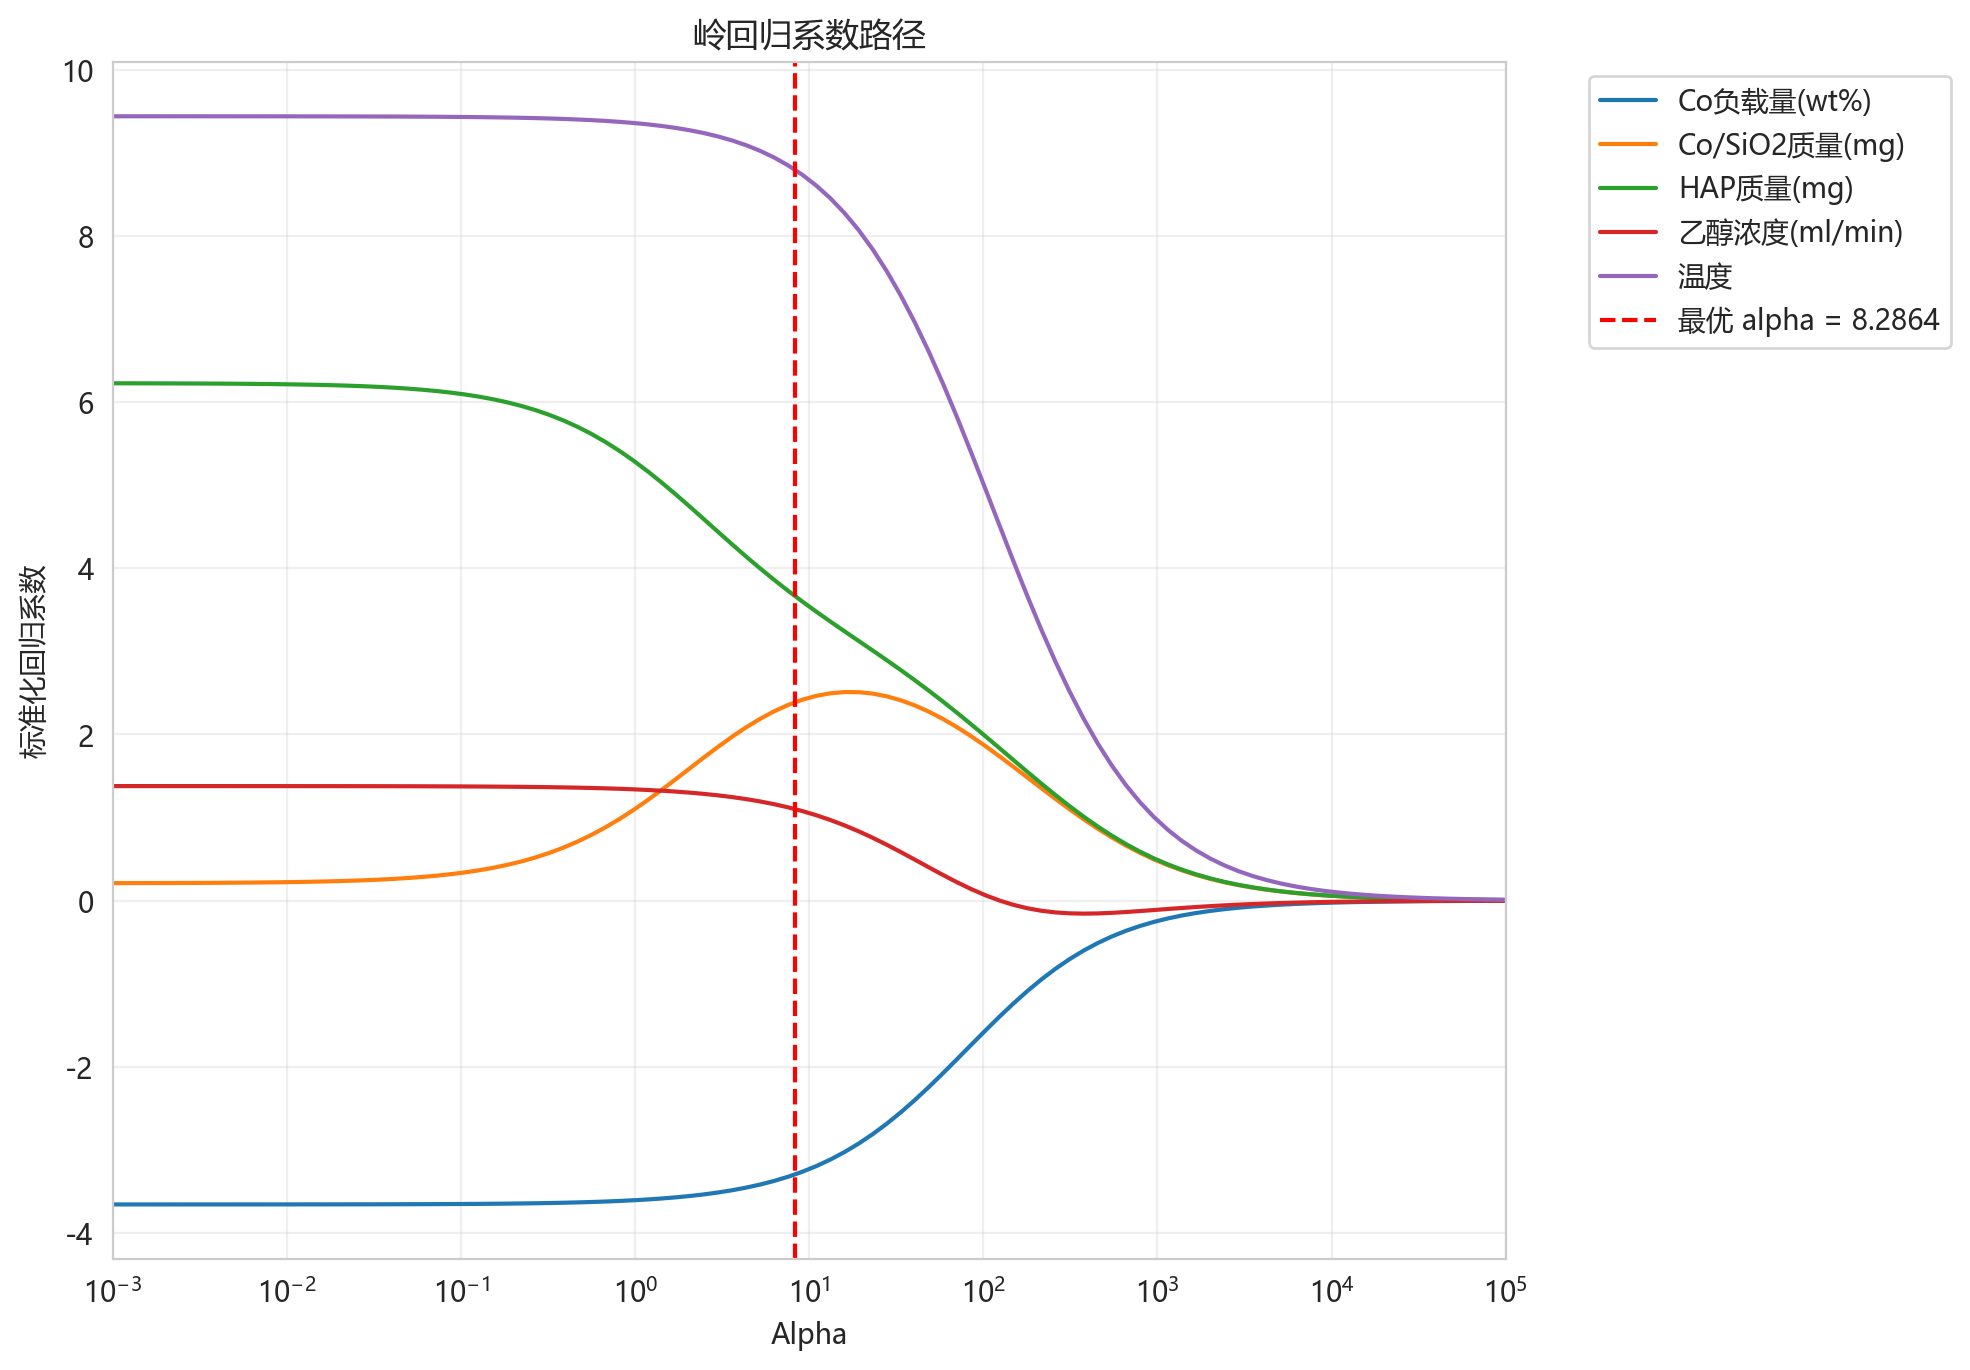
\includegraphics [scale=0.6]{图/ling-xuanzexing.png}
	\caption{ \( \text{C}_4 \) 烯烃选择性岭回归系数路径} 
	\label{fig:1}
\end{figure}

\begin{table}[!htbp]
	\caption{C4烯烃选择性模型的标准化回归系数}
	\centering
	\begin{tabular}{l c}
		\hline
		\multicolumn{1}{c}{\textbf{特征名称}} & \textbf{标准化回归系数} \\
		\hline
		Co负载量(wt\%)      & -3.4383 \\
		Co/SiO2质量(mg)     & 2.1327 \\
		HAP质量(mg)         & 4.0744 \\
		乙醇浓度(ml/min)    & 1.2088 \\
		温度 (°C)               & 9.0609 \\
		\hline
		\label{tab:ridge_selectivity}
	\end{tabular}
\end{table}



 %插入附录   Appendix.tex



\end{document}